%%%%%%%%%%%%%%%%%%%%%%%%%%%%%%%%%%%%%%%%%%%%%%%%%%%
%
%  New template code for TAMU Theses and Dissertations starting Fall 2012.  
%  For more info about this template or the 
%  TAMU LaTeX User's Group, see http://www.howdy.me/.
%
%  Author: Wendy Lynn Turner 
%
%%%%%%%%%%%%%%%%%%%%%%%%%%%%%%%%%%%%%%%%%%%%%%%%%%%

\documentclass[12pt,aas_macros]{report} 
\usepackage[letterpaper]{geometry} \geometry{verbose,tmargin=1.25in,bmargin=1.25in,lmargin=1.4in,rmargin=1.15in} 
\usepackage[doublespacing]{setspace} 
\usepackage{tocloft} 
\usepackage[rm, tiny,center, compact]{titlesec} 
\usepackage{indentfirst} 
\usepackage{etoolbox} 
\usepackage{tocvsec2} 
\usepackage[titletoc]{appendix} 
\usepackage{appendix} 
\usepackage{tamuconfig} 
\usepackage{rotating} 
\usepackage[round]{natbib} 
\usepackage{aas_macros} 
\usepackage{epsfig} 
\usepackage{graphicx} 
\usepackage{float} 
\usepackage{booktabs} 
\usepackage{threeparttable} 
\usepackage{amsmath} 
\usepackage{pdflscape} 
\usepackage[hang,flushmargin]{footmisc}
\long\def\symbolfootnote[#1]#2 {\begingroup%
\def\thefootnote{\fnsymbol{footnote}}\footnote[#1]{#2}\endgroup}


% Added to fix issues with pdf searching in some versions of LaTeX
\usepackage[T1]{fontenc}\usepackage{lmodern}
%%%%%%%%%%%%%%%%%%%%%%%%%%%%%

% Hyperref setup below.  You should be able to get away with using uncommenting just the first line.
%\usepackage[hidelinks]{hyperref}

% if \usepackage[hidelinks]{hyperref} doesn't work try this.
% \usepackage{hyperref}  % Hidelinks is an option that removes link visiability.  TAMU Thesis Offices prefers to not see the links. But often doesn't work.  
% 
% \hypersetup{
%     colorlinks=true,
%     linkcolor=black,
%     citecolor=black,
%     filecolor=black,
%     urlcolor=black,
% }
%%%%%%%  End of hyperref setup.  One of these two options should work, but my motto with hyperref is when in doubt, comment it out!
%%%%%%%%%  This hopefully fixes the problem with vertical spacing of section headings at the top of the page..  Commented out in 1.0.7
% \preto\section{%
% \ifnum\value{section}>0\addtocontents{toc}{\vskip-6pt}\fi
% }
% \preto\subsection{%
% \ifnum\value{subsection}=0\addtocontents{toc}{\vskip-6pt}\fi
% \ifnum\value{subsection}>0\addtocontents{toc}{\vskip-6pt}\fi
% } 
%%%%%%%%%%%%%%%%%%%%%%%%%%%%%%%%%%%%%%%%%%%%%%%%%%%%%%

\begin{document}

\renewcommand{\tamumanuscripttitle}{The Precision Analysis of Time Series Photometry and its Application to Searches for Pre-Main-Sequence Objects}
\renewcommand{\tamupapertype}{Dissertation}
\renewcommand{\tamufullname}{Ryan James Oelkers}
\renewcommand{\tamudegree}{Doctor of Philosophy}
\renewcommand{\tamuchairone}{Lucas M. Macri}
% Uncomment out the next line if you have co-chairs.  You will also need to edit the titlepage.tex file.
%\newcommand{\tamuchairtwo}{Additional Chair Name}
\renewcommand{\tamumemberone}{Darren L. DePoy}
\newcommand{\tamumembertwo}{Jennifer L. Marshall}
\newcommand{\tamumemberthree}{Lifan Wang}
\newcommand{\tamumemberfour}{James Long}
\renewcommand{\tamudepthead}{George R. Welch}
\renewcommand{\tamugradmonth}{May}
\renewcommand{\tamugradyear}{2016}
\renewcommand{\tamudepartment}{Physics}




%%%%%%%%%%%%%%%%%%%%%%%%%%%%%%%%%%%%%%%%%%%%%%%%%%%
%
%  New template code for TAMU Theses and Dissertations starting Fall 2012.  
%  For more info about this template or the 
%  TAMU LaTeX User's Group, see http://www.howdy.me/.
%
%  Author: Wendy Lynn Turner 
%	 Version 1.0 
%  Last updated 8/5/2012
%
%%%%%%%%%%%%%%%%%%%%%%%%%%%%%%%%%%%%%%%%%%%%%%%%%%%
%%%%%%%%%%%%%%%%%%%%%%%%%%%%%% 
%% TITLE PAGE
%% The values get updated automatically.  Please do not make changes to this file other than adding/deleting committee members where necessary.
%%%%%%%%%%%%%%%%%%%%%%%%%%%%%%
\providecommand{\tabularnewline}{\\}
\begin{titlepage}
	\begin{center}
		\MakeUppercase{\tamumanuscripttitle} \vspace{4em}
		
		A \tamupapertype
		
		by
		
		\MakeUppercase{\tamufullname}
		
		\vspace{4em}
		\begin{singlespace}
			
			Submitted to the Office of Graduate and Professional Studies of \\
			Texas A\&M University \\
			
			in partial fulfillment of the requirements for the degree of \\
		\end{singlespace}
		
		\MakeUppercase{\tamudegree} \par
	\end{center}
	\vspace{2em} 
	\begin{singlespace}
		\begin{tabular}
			{ll} & \tabularnewline & \cr
			
			% If you have Co-Chairs comment out the 'Chair of Committee' line below and uncomment the 'Co-Chairs of Committee' line.
			Chair of Committee, & \tamuchairone\tabularnewline
			
			%Co-Chairs of Committee, & \tamuchairone\tabularnewline & \tamuchairtwo\tabularnewline
			Committee Members, & \tamumemberone\tabularnewline & \tamumembertwo\tabularnewline & \tamumemberthree\tabularnewline Head of Department, & \tamudepthead\tabularnewline
		\end{tabular}
	\end{singlespace}
	\vspace{3em}
	\begin{center}
		\tamugradmonth \hspace{2pt} \tamugradyear
		
		\vspace{3em}
		
		Major Subject: \tamudepartment \par \vspace{3em} Copyright \tamugradyear \hspace{.5em}\tamufullname \par
	\end{center}
\end{titlepage}
\pagebreak{}
 % This is simply a file that formats and adds your titlepage, please do not edit this unless you have a specific need. .
%%%%%%%%%%%%%%%%%%%%%%%%%%%%%%%%%%%%%%%%%%%%%%%%%%%
%
%  New template code for TAMU Theses and Dissertations starting Fall 2012.  
%  For more info about this template or the 
%  TAMU LaTeX User's Group, see http://www.howdy.me/.
%
%  Author: Wendy Lynn Turner 
%	 Version 1.0 
%  Last updated 8/5/2012
%
%%%%%%%%%%%%%%%%%%%%%%%%%%%%%%%%%%%%%%%%%%%%%%%%%%%
%%%%%%%%%%%%%%%%%%%%%%%%%%%%%%%%%%%%%%%%%%%%%%%%%%%%%%%%%%%%%%%%%%%%%
%%                           ABSTRACT 
%%%%%%%%%%%%%%%%%%%%%%%%%%%%%%%%%%%%%%%%%%%%%%%%%%%%%%%%%%%%%%%%%%%%%

\chapter*{ABSTRACT}
\addcontentsline{toc}{chapter}{ABSTRACT} % Needs to be set to part, so the TOC doesnt add 'CHAPTER ' prefix in the TOC.

\pagestyle{plain} % No headers, just page numbers
\pagenumbering{roman} % Roman numerals
\setcounter{page}{2}

\indent The distribution of massive clusters of galaxies depends strongly on the total cosmic mass density, the mass variance, and the dark energy equation of state. As such, measures of galaxy clusters can provide constraints on these parameters and even test models of gravity, but only if observations of clusters can lead to accurate estimates of their total masses. Here, we carry out a study to investigate the ability of a blind spectroscopic survey to recover accurate galaxy cluster masses through their line-of-sight velocity dispersions (LOSVD) using probability based and machine learning methods. We focus on the Hobby Eberly Telescope Dark Energy Experiment (HETDEX), which will employ new Visible Integral-Field Replicable Unit Spectrographs (VIRUS), over 420 \degsq\ on the sky with a 1/4.5 fill factor. VIRUS covers the blue/optical portion of the spectrum ($3500-5500~\AAA$), allowing surveys to measure redshifts for a large sample of galaxies out to $z < 0.5$ based on their absorption or emission (\eg, [\ion{O}{II}], \ion{Mg}{II}, \ion{Ne}{V}) features. We use a detailed mock galaxy catalog from a semi-analytic model to simulate surveys observed with VIRUS, including: (1) Survey, a blind, HETDEX-like survey with an incomplete but uniform spectroscopic selection function; and (2) Targeted, a survey which targets clusters directly, obtaining spectra of all galaxies in a VIRUS-sized field. For both surveys, we include realistic uncertainties from galaxy magnitude and line-flux limits. We benchmark both surveys against spectroscopic observations with ``perfect" knowledge of galaxy line-of-sight velocities. With Survey observations, we can recover cluster masses to $\sim0.1$ dex which can be further improved to $<0.1$ dex with Targeted observations. This level of cluster mass recovery provides important measurements of the intrinsic scatter in the optical richness-cluster mass relation, and enables constraints on the key cosmological parameter, $\sigma_8$, to to $<20$\%.

As a demonstration of the methods developed previously, we present a pilot survey with integral field spectroscopy of ten galaxy clusters optically selected from the Sloan Digital Sky Survey's DR8 at $z=0.2-0.3$. Eight of the clusters are rich ($\lambda>60$) systems with total inferred masses $(1.58-17.37) \times 10^{14}$ \Msol\ ($M_{200c}$), and two are poor ($\lambda<15$) systems with inferred total masses $\sim0.5 \times 10^{14}$ \Msol\ ($M_{200c}$). We use the Mitchell Spectrograph, (formerly the VIRUS-P spectrograph, a prototype of the HETDEX VIRUS instrument) located on the McDonald Observatory 2.7m telescope, to measure spectroscopic redshifts and line-of-sight velocities of the galaxies in and around each cluster, determine cluster membership and derive LOSVDs. We test both a LOSVD-cluster mass scaling relation and a machine learning based approach to infer total cluster mass. After comparing the cluster mass estimates to the literature, we use these independent cluster mass measurements to estimate the absolute cluster mass scale, and intrinsic scatter in the optical richness-mass relationship. We measure the intrinsic scatter in richness at fixed cluster mass to be $\sigma_{M|\lambda} = 0.27\pm0.07$ dex in excellent agreement with previous estimates of $\sigma_{M|\lambda} \sim 0.2-0.3$ dex. We discuss the importance of the data used to train the machine learning methods and suggest various strategies to import the accuracy of the bias (offset) and scatter in the optical richness-cluster mass relation. This demonstrates the power of blind spectroscopic surveys such as HETDEX to provide robust cluster mass estimates which can aid in the determination of cosmological parameters and help to calibrate the observable-mass relation for future photometric large area-sky surveys.
\pagebreak{}

%%%%%%%%%%%%%%%%%%%%%%%%%%%%%%%%%%%%%%%%%%%%%%%%%%%%
%
%  New template code for TAMU Theses and Dissertations starting Fall 2012.  
%  For more info about this template or the 
%  TAMU LaTeX User's Group, see http://www.howdy.me/.
%
%  Author: Wendy Lynn Turner 
%	 Version 1.0 
%  Last updated 8/5/2012
%
%%%%%%%%%%%%%%%%%%%%%%%%%%%%%%%%%%%%%%%%%%%%%%%%%%%

%%%%%%%%%%%%%%%%%%%%%%%%%%%%%%%%%%%%%%%%%%%%%%%%%%%%%%%%%%%%%%%%%%%%%%
%%                           DEDICATION
%%%%%%%%%%%%%%%%%%%%%%%%%%%%%%%%%%%%%%%%%%%%%%%%%%%%%%%%%%%%%%%%%%%%%
\chapter*{DEDICATION}
\addcontentsline{toc}{chapter}{DEDICATION}  % Needs to be set to part, so the TOC doesnt add 'CHAPTER ' prefix in the TOC.



\indent This is an optional page.  Lorem ipsum dolor sit amet, consectetur adipiscing elit. Integer lectus quam, condimentum quis bibendum eu, sollicitudin eget lacus. Praesent non sodales odio. Class aptent taciti sociosqu ad litora torquent per conubia nostra, per inceptos himenaeos. Nulla ac luctus sapien. Morbi cursus sapien eget lorem fermentum hendrerit. Nam ac erat dui, in cursus velit. Vivamus hendrerit porttitor nisi, ut porttitor lorem volutpat eget. In ligula ligula, euismod ut condimentum sit amet, pulvinar sit amet diam. Pellentesque interdum, ipsum ullamcorper consequat dignissim, sem arcu egestas mauris, vitae interdum sem tortor ut ante. Nunc blandit laoreet nisi, non rutrum lorem hendrerit quis. Cras nunc diam, convallis et feugiat at, auctor id libero. Nunc facilisis massa eu eros imperdiet vestibulum. Vestibulum ante ipsum primis in faucibus orci luctus et ultrices posuere cubilia Curae; Donec non velit vitae tortor blandit semper.

Etiam vitae dolor nulla. Ut eros odio, rhoncus eget placerat vitae, elementum ac ante. Proin vitae odio eu nisl pharetra mattis. Pellentesque habitant morbi tristique senectus et netus et malesuada fames ac turpis egestas. Phasellus fermentum lacus consectetur neque consequat ullamcorper. Cras blandit urna non dui consequat molestie. Curabitur viverra nibh at nisi semper faucibus. Nam egestas mauris a enim dignissim nec consectetur tortor rutrum. Mauris at nisi in est luctus congue ut mattis est. Ut pretium, mi quis elementum cursus, ante eros suscipit ligula, ut porttitor elit leo sed turpis. Nam sed dui ligula.


\pagebreak{}

%%%%%%%%%%%%%%%%%%%%%%%%%%%%%%%%%%%%%%%%%%%%%%%%%%%
%
%  New template code for TAMU Theses and Dissertations starting Fall 2012.  
%  For more info about this template or the 
%  TAMU LaTeX User's Group, see http://www.howdy.me/.
%
%  Author: Wendy Lynn Turner 
%	 Version 1.0 
%  Last updated 8/5/2012
%
%%%%%%%%%%%%%%%%%%%%%%%%%%%%%%%%%%%%%%%%%%%%%%%%%%%


%%%%%%%%%%%%%%%%%%%%%%%%%%%%%%%%%%%%%%%%%%%%%%%%%%%%%%%%%%%%%%%%%%%%%%
%%                           ACKNOWLEDGEMENTS
%%%%%%%%%%%%%%%%%%%%%%%%%%%%%%%%%%%%%%%%%%%%%%%%%%%%%%%%%%%%%%%%%%%%%
\chapter*{ACKNOWLEDGEMENTS}
\addcontentsline{toc}{chapter}{ACKNOWLEDGEMENTS}  % Needs to be set to part, so the TOC doesnt add 'CHAPTER ' prefix in the TOC.


\indent 
I would like to express my most sincere gratitude to my advisor, Dr. Casey Papovich, for the continual support of my research pursuits, his unwavering patience, the kind and sometimes stern words, his encouragement, and vast knowledge. His support and guidance have helped me throughout all stages of researching and writing this thesis. I can confidently say that I would not have arrived alone, and I cannot imagine a better advisor for my study.

To my thesis committee: Dr. Wolfgang Bangerth, Dr. Louis Strigari, and Dr. Nicholas Suntzeff who were always at the ready with invaluable comments and encouragement, and for never shying away from asking the hard questions which pushed me to new heights. Thank you.

I thank my fellow graduate students with whom I spent so much of my life. Thank you for all the stimulating discussions, homework and research help, encouragement, and the fun over the previous six years.

Finally, I could not have accomplished this with out the love and support of my family and friends. I am so very fortunate that there are too many to name, but thank you for always believing in me, even when I did not believe in myself. Thank you for being a distraction when I needed it, and for being a support system when I needed it. Thank you for your unwavering optimism, and your tireless work. I can never repay you. Thank you.
\pagebreak{}
%%%%%%%%%%%%%%%%%%%%%%%%%%%%%%%%%%%%%%%%%%%%%%%%%%%
%
%  New template code for TAMU Theses and Dissertations starting Fall 2012.  
%  For more info about this template or the 
%  TAMU LaTeX User's Group, see http://www.howdy.me/.
%
%  Author: Wendy Lynn Turner 
%	 Version 1.0 
%  Last updated 8/5/2012
%
%%%%%%%%%%%%%%%%%%%%%%%%%%%%%%%%%%%%%%%%%%%%%%%%%%%

%%%%%%%%%%%%%%%%%%%%%%%%%%%%%%%%%%%%%%%%%%%%%%%%%%%%%%%%%%%%%%%%%%%%%%
%%                           NOMENCLATURE
%%%%%%%%%%%%%%%%%%%%%%%%%%%%%%%%%%%%%%%%%%%%%%%%%%%%%%%%%%%%%%%%%%%%%

\chapter*{NOMENCLATURE}
\addcontentsline{toc}{chapter}{NOMENCLATURE}  % Needs to be set to part, so the TOC doesnt add 'CHAPTER ' prefix in the TOC.

\begin{tabular}{ll}
B/CS  & Bryan/College Station\tabularnewline
HSUS & Humane Society of the United States\tabularnewline
P & Pressure\tabularnewline
T  & Time\tabularnewline
TVA & Tennessee Valley Authority\tabularnewline
TxDOT \hfill{}\hfill{}\hfill{}\hfill{}\hfill{}\hfill{}\hfill{}\hfill{} & \multicolumn{1}{l}{Texas Department of Transportation}\tabularnewline
\end{tabular}

\vspace{2em}

This page is optional.

\pagebreak{}

%%%%%%%%%%%%%%%%%%%%%%%%%%%%%%%%%%%%%%%%%%%%%%%%%%%
%
%  New template code for TAMU Theses and Dissertations starting Fall 2012.  
%  For more info about this template or the 
%  TAMU LaTeX User's Group, see http://www.howdy.me/.
%
%  Author: Wendy Lynn Turner 
%	 Version 1.7X
%  Modified by Jimmy
%
%%%%%%%%%%%%%%%%%%%%%%%%%%%%%%%%%%%%%%%%%%%%%%%%%%%
%%%%%%%%%%%%%%%%%%%%%%%%%%%%%%%%%%%%%%%%%%%%%%%%%%%%%%%%%%%%%%%%%%%%%%
%%       TABLE OF CONTENTS
%%%%%%%%%%%%%%%%%%%%%%%%%%%%%%%%%%%%%%%%%%%%%%%%%%%%%%%%%%%%%%%%%%%%%
% single-space sections in Table of Contents  - commented in version 1.7
%\renewcommand{\cftsecafterpnum}{\vskip0.5\baselineskip}
%\renewcommand{\cftsubsecafterpnum}{\vskip0.5\baselineskip}
%\renewcommand{\cftsubsubsecafterpnum}{\vskip0.5\baselineskip}
%%%%%%%%%%%%%%%%%%%%%%%%%%%%%%%%%%%%%%%%%%%%%%%%%%%

\phantomsection
\addcontentsline{toc}{chapter}{TABLE OF CONTENTS}  

\begin{singlespace}
\renewcommand\contentsname{\normalfont} {\centerline{TABLE OF CONTENTS}}

%\setcounter{tocdepth}{4} % This puts \subsubsection[]{×} in your List of Tables.  The default is 3.


%%%%%%%%%%%%%  Adds Page above the page number in TOC
\setlength{\cftaftertoctitleskip}{1em}
\renewcommand{\cftaftertoctitle}{%
\hfill{\normalfont {Page}\par}}



\tableofcontents

\end{singlespace}

\pagebreak{}

%%%%%%%%%%%%%%%%%%%%%%%%%%%%%%%%%%%%%%%%%%%%%%%%%%%%%%%%%%%%%%%%%%%%%%
%%                           LIST OF FIGURES
%%%%%%%%%%%%%%%%%%%%%%%%%%%%%%%%%%%%%%%%%%%%%%%%%%%%%%%%%%%%%%%%%%%%%

\phantomsection
\addcontentsline{toc}{chapter}{LIST OF FIGURES}  

\renewcommand{\cftloftitlefont}{\center\normalfont\MakeUppercase}

\setlength{\cftbeforeloftitleskip}{-12pt} %% Positions the LOF title vertically to match the chapter titles
\renewcommand{\cftafterloftitleskip}{12pt}


\renewcommand{\cftafterloftitle}{%
\\[4em]\mbox{}\hspace{2pt}FIGURE\hfill{\normalfont Page}\vskip\baselineskip}

\begingroup


\begin{center}
\begin{singlespace}
%% These values make the lof table entries appear double spaced between.
\setlength{\cftbeforechapskip}{0.4cm}
\setlength{\cftbeforesecskip}{0.30cm}
\setlength{\cftbeforesubsecskip}{0.30cm}
\setlength{\cftbeforefigskip}{0.4cm}
\setlength{\cftbeforetabskip}{0.4cm} 

%\listoffigures
\begingroup
\renewcommand*{\addvspace}[1]{}
\listoffigures
\endgroup

\end{singlespace}
\end{center}

\pagebreak{}


%%%%%%%%%%%%%%%%%%%%%%%%%%%%%%%%%%%%%%%%%%%%%%%%%%%%%%%%%%%%%%%%%%%%%%
%%                           lIST OF TABLES
%%%%%%%%%%%%%%%%%%%%%%%%%%%%%%%%%%%%%%%%%%%%%%%%%%%%%%%%%%%%%%%%%%%%%%
%
\phantomsection
\addcontentsline{toc}{chapter}{LIST OF TABLES}  

\renewcommand{\cftlottitlefont}{\center\normalfont\MakeUppercase}

\setlength{\cftbeforelottitleskip}{-12pt} %% Positions the LOT title vertically to match the chapter titles

\renewcommand{\cftafterlottitleskip}{12pt}


\renewcommand{\cftafterlottitle}{%
\\[4em]\mbox{}\hspace{4pt}TABLE\hfill{\normalfont Page}\vskip\baselineskip}

\begin{center}
\begin{singlespace}

%% These values make the lot table entries appear double spaced between.
\setlength{\cftbeforechapskip}{0.4cm}
\setlength{\cftbeforesecskip}{0.30cm}
\setlength{\cftbeforesubsecskip}{0.30cm}
\setlength{\cftbeforefigskip}{0.4cm}
\setlength{\cftbeforetabskip}{0.4cm}

%\listoftables 
\begingroup
\renewcommand*{\addvspace}[1]{}
\listoftables
\endgroup

\end{singlespace}
\end{center}
\endgroup
\pagebreak{}  % Need this for the pagenumbering to be correct.   % This is simply a file that formats and adds your toc, lof, and lot, please do not edit this unless you have a specific need. .

%%%%%%%%%%%%%%%%%%%%%%%%%%%%%%%%%%%%%%%%%%%%%%%%%%%
%
%  New template code for TAMU Theses and Dissertations starting Fall 2012.  
%  For more info about this template or the 
%  TAMU LaTeX User's Group, see http://www.howdy.me/.
%
%  Author: Wendy Lynn Turner 
%	 Version 1.0 
%  Last updated 8/5/2012
%
%%%%%%%%%%%%%%%%%%%%%%%%%%%%%%%%%%%%%%%%%%%%%%%%%%%

%%%%%%%%%%%%%%%%%%%%%%%%%%%%%%%%%%%%%%%%%%%%%%%%%%%%%%%%%%%%%%%%%%%%%%
%%                           SECTION I
%%%%%%%%%%%%%%%%%%%%%%%%%%%%%%%%%%%%%%%%%%%%%%%%%%%%%%%%%%%%%%%%%%%%%


\pagestyle{plain} % No headers, just page numbers
\pagenumbering{arabic} % Arabic numerals
\setcounter{page}{1}


\renewcommand*{\thefootnote}{\fnsymbol{footnote}}
\chapter[Introduction: The Importance of Research]{\uppercase {Introduction: The Importance of Research}\symbolfootnote[1]{Reprinted with permission from ``Introduction: The Importance of Research'' by AUTHOR et al., 2015. The Astrophysical Journal, Volume XYZ, Issue X, article id. XY, XY pp., Copyright 20XX by the American Astronomical Society.} }
\renewcommand*{\thefootnote}{\arabic{footnote}}
\setcounter{footnote}{0}


Clusters of galaxies form the largest bound objects in the universe, and as such their study is a cornerstone in modern day astronomy. First recognized by 19th century astronomers, their place in astronomical canon was solidified when Edwin Hubble proofed their constituent nebulae where not bound to the Milky Way \citep{Hubble1926} but collections of stars similar to the Milky Way. Work to understand their nature and origin began in ernest when \cite{Hubble1931} used the virial theorem and the galaxy velocities in the centers of the Virgo \citep{Smith1936} and Coma \citep{Zwicky1933} clusters to derive their masses. The immense mass derived exceeded the total stellar mass contributed by all galaxies many times over. This lead Zwicky to theorize the existence of large amounts of non-luminous matter, and coining the term ``dark matter'' (DM), which we still use today.  

Modern astronomy gives the composition of galaxy clusters in three many parts. The galaxies themselves comprise the most obvious feature, and contain a large portion (but not the entirety) of the luminous matter (stars) in the cluster. The intracluster medium (ICM) is the space between the cluster galaxies and is composed many of ordinary matter (baryons) which are super heated to tens of thousands of kelvin. The ICM contains the bulk of the cluster's baryonic matter, and while it is very hot, it is not very dense, with a typical value of $10^{-3}$ particles per cubic centimeter. The majority of the cluster's mass is located in the DM halo which surrounds the cluster. 

Thought to form out of the primordial density fluctuations in the very early universe, the investigation of their formation and growth began in the 1960s. Soon thereafter, the hierarchical model of structure formation \citep{Press1974, Gott1975, White1978} was introduced. It suggests the first stars and stellar clumps grew first then subsequently merged together with dark matter and other gas clumps to form the first galaxies which then continued to merge and grow into the clusters and large scale structures we see today. This accretion of smaller systems is thought to be driven by the gravity of the DM associated with the cluster. Of course, many complicated astrophysical processes are at work during cluster growth and similarly complicated theoretical models seek to explain these processes. For a detailed review of cluster formation see \cite{Kravtsov2012}.

The number and distribution of galaxy clusters across the sky is the finger print of the cosmology imprinted on the universe at its birth. To uncover the underlying cosmology a detailed understanding of the astrophysical processes that describe the motion of constituent galaxies and their impact on the ICM is required. So, galaxy clusters stand at the intersection of cosmology and astrophysics. 

\section{Cluster Cosmology}
The current concordance cosmology is a parametrization of the Big Bang cosmological model where the universe contains a cosmological constant ($\Lambda$; often referred to as dark energy) and cold dark matter (CDM). It is often characterized by six parameters; the Hubble Constant ($H_0$), the baryonic matter density ($\Omega_b$), the dark matter density ($\Omega_c$), the dark energy density ($\Omega_\Lambda$); the normalization of the power spectrum ($\sigma_8$); the spectral index of the power spectrum ($n_s$). Galaxy clusters are sensitive probes of $\Omega_m$, the total mass ($\Omega_b + \Omega_c$) density in the universe, through tracing the peaks in the universal matter density often referred to as the power spectrum of matter density fluctuations or the matter power spectrum and $\sigma_8$ by the comparison of the number density of observed halos to that predicted in cosmological models. %Although, in reality, one measures $\sigma_8\Omega_m^\alpha$, where the value of $\alpha$ depends on the masses of the halos considered.

The determination of cosmological parameters is done by comparing the number of galaxy clusters per unit mass per unit comoving volume ($n(M,z)$) to models. See \cite{Allen2011} for a comprehensive review or \cite{Murray2013} for a more practical approach. $n(M,z)$, referred to as the halo mass function (HMF) captures the number evolution through a function which defines the particular model used. Early work by \cite{Press1974} and \cite{Bond1991} which assumed spherical halos, have largely been replaced by more modern fitting functions which, at the expense of an analytical solution, provide more accurate results when fit to simulation data. See \cite{Murray2013} for a review of the most common fitting functions used. Through this approach, the two parameters which clusters are most sensitive to, $\Omega_m$ and $\sigma_8$ are in reality measured as $\sigma_8\Omega_m^\alpha$, where the value of $\alpha$ depends on the masses of the halos considered. The degeneracy is broken through the evolution of the HMF as a function of redshift. 

The $\Lambda$CDM model of cosmology makes explicit predictions about the number and masses of galaxy clusters throughout the universe. Connecting these predictions to a set of, sufficiently large in size, observed clusters remains a principal problem. Specifically, the largest threat to modern, precision, cluster cosmology is not the identification of large numbers of clusters (the total number of clusters known is only going up) but the accurate recovery of galaxy cluster mass. This problem extends to both the very rich clusters (those with high mass) and, importantly, the poor clusters (those with low mass) as the relationship between galaxy cluster mass and many of the observables which trace mass is not well understood for such low mass clusters.

\section{State of Play}
As mass is not a direct observable, a lot of work is underway to characterize galaxy cluster masses with an observable feature of galaxy clusters. In this section, we will briefly touch on a few of the ways cluster mass is determined, and address any short comings the method may have. Generally, the methods fall into two distinct camps, simulation based and direct or statistical calibration. The goal is to constrain, as best possible, $P(X|M,z)$ or the probability ($P$) that a galaxy cluster of given mass ($M$) located at redshift ($z$) using observable parameter ($X$).

One could use various simulations to attempt to calibrate this observable--mass relation \citeeg{Vanderlinde2010, Sehgal2011}. However, the primary challenge to this method is the incomplete understanding of the baryonic physics which take place in galaxy cluster environments. While there have been (and continue to be) many improvements in the accuracy and power of simulations it is doubtful that in the coming years they will reach the accuracy level required to the point where the observable--mass relation is dominated only by statistics \citep{Weinberg2013}. 
 
The second broad camp is the direct calibration of cluster masses. This recipe has two distinct but not always independent tracks. The ``direct'' method uses the direct observations of a small set of clusters and then uses known mass estimators, X-ray hydrostatic or weak lensing (WL) as examples, which provide a ``true'' mass. This directly calibrates the observable--mass relation which is then applied to a much larger sample. The complications lie in that the ``true'' masses are in fact estimations, and the methods used to recover these masses are subject to their own limitations. X-ray hydrostatic estimations assume hydrostatic equilibrium \citeeg{Mantz2015} which may only be valid for a very small number and range of cluster masses. The Sunyaev--Zel’dovich (SZ; \citealt{Sunyaev1972}) effect, which uses the up--scattering of cosmic microwave background (CMB) photons to estimate cluster masses, provides accurate estimations of mass, but the ability to detect low mass galaxy clusters is currently limited by technology \citeeg{Carlstrom2002a}. WL estimates are, in principle, correct in the mean, but they suffer from signal-to-noise requirements, limiting their usefulness in low mass clusters, and potentially suffer from line-of-sight effects as the effect is sensitive to all mass along the line of sight. Virial mass estimators which determine the cluster mass based on the motions of the member galaxies is promising in that it is a direct measurement of the depth of clusters potential well, but suffers from systematics due to cluster formation physics which disrupts the velocity field.
 
The statistical method of determining galaxy cluster mass relies not on direct measurements of individual clusters but the calibration of observables for the entire sample which correlate with cluster mass. One example is the spatial clustering of the galaxy clusters themselves. See \cite{Weinberg2013} for a comprehensive review. In practice, it will be a combination of the three methods touched on that will provide the most reliable determination of cluster masses. 

Virial mass estimators, specifically, can be applied in both a direct and statistical fashion. Currently, the accuracy of such a method, especially to the level required for today's precision cosmology, is not well constrained. In the coming years large spectroscopic surveys will provide enough coverage, and so these methods warrant further investigation \citeeg{Saro2013}.

\section{Cluster Surveys in the near-future}
In the coming years, many large surveys will add further statistical advantages to the determination of cosmological parameters using galaxy clusters. At their completion, the South Pole Telescope (SPT; \citealt{Carlstrom2011}) and the Atacama Cosmology Telescope (ACT; \citealt{Swetz2011}) are expected to find approximately one thousand clusters using observations in the millimeter combined with the SZ effect. Attempts are already underway to calibrate these observations using subsamples of clusters (approximately 100 cluster candidates and 60 clusters respectively) and other observables such as virial estimates or X-ray temperature measurements \citeeg{Sifon2013, Bocquet2015}. 

X-ray identified clusters, up until today, have mostly been observed fortuitously through targeted \textit{Chandra} or \textit{XMM-Newton} observations. That is soon to change with the \textit{eROSITA} telescope onboard the Spektrum-Roentgen-Gamma Mission, which will perform an all--sky survey during its four year mission and detect an estimated 50,000 or more clusters.

Large optical surveys such as the Dark Energy Survey (DES; \citealt{DES2005}) and the Large Synoptic Survey Telescope (LSST) will survey enormous portions of the sky extremely deeply and will identify vast numbers of clusters using optical selection methods \citeeg{Rykoff2014, Rozo2014}. However, the majority of these surveys will be photometric, and any spectral information will be obtained from preexisting datasets. And while it is possible to estimate cluster masses using photometric redshifts, primarily through the richness--mass relation, \citeeg{Rykoff2012, Rykoff2014}, spectroscopic followup is required to both better calibrate the relation and to obtain the level of precision needed to compete with other mass estimators. 

\subsection{Impact of This Work}
As the sample of known clusters grows to many tens of thousands, spectroscopic followup becomes unfeasible. Large spectroscopic surveys will be required to reduce systematics to a level that will allow accurate mass estimations using virial methods. The Hobby Eberly Dark Energy Experiment (HETDEX; \citealt{Hill2008}) is a forthcoming blind spectroscopic survey that could potentially be used to accurately calibrate the observable--mass relation for a significant number of galaxy clusters at both extremes of the mass scale. HETDEX is designed to measure the dark energy equation of state at $z\sim2$, and so the applicability to galaxy cluster science has not yet been investigated.

Given how much progress could be made with HETDEX, this work seeks to address this issue in two ways. First, using a set of state-of-the-art simulations we will simulate the observing strategy of HETDEX to determine the number and nature of clusters that might be observed. See Section~\ref{sec:hetdex project}. This is done in four distinct ways and in each part we will measure the dynamical properties, such as redshift, LOSVD, and mass of the clusters. First we will use targeted observations and perfect knowledge of the observed galaxy clusters, which includes center, membership, and number to recover the desired properties. Secondly, we will assume that we know the location but not the center, membership, or number of constituent galaxies. Then we will employ the HETDEX observing strategy, including realistic pointing pattern, observational magnitude constraints, and spectral sensitivity limits to generate a set of realistic observations which are then used with perfect and less than perfect knowledge scenarios to determine the cluster properties. 

In all cases, we will attempt to characterize the observable--mass relation (or relations) to better understand the dominate sources of uncertainty when using HETDEX like observations. This will enable us to more fully understand and constrain the HMF which, in turns, allows us to make more accurate measurements of the cosmological parameters traced by galaxy clusters.

The second effort of this work, outlined in Section~\ref{sec:vp project}, will use targeted spectroscopic observations of ten nearby clusters with the Mitchell Spectrograph (formerly known as VIRUS-P; \citealt{Hill2008a}), an integral field unit (IFU) in a square array of 246 $4.24''$ diameter optical fibers, to test some of the methods used in the first method. This will provide insight in how the observable--mass relation may be improved through followup observations of targeted clusters.

%%%%%%%%%%%%%%%%%%%%%%%%%%%%%%%%%%%%%%%%%%%%%%%%%%%
%
%  New template code for TAMU Theses and Dissertations starting Fall 2012.  
%  For more info about this template or the 
%  TAMU LaTeX User's Group, see http://www.howdy.me/.
%
%  Author: Wendy Lynn Turner 
%	 Version 1.0 
%  Last updated 8/5/2012
%
%%%%%%%%%%%%%%%%%%%%%%%%%%%%%%%%%%%%%%%%%%%%%%%%%%%

%%%%%%%%%%%%%%%%%%%%%%%%%%%%%%%%%%%%%%%%%%%%%%%%%%%%%%%%%%%%%%%%%%%%%%%
%%%                           SECTION II
%%%%%%%%%%%%%%%%%%%%%%%%%%%%%%%%%%%%%%%%%%%%%%%%%%%%%%%%%%%%%%%%%%%%%%

\chapter{\uppercase {Literature Review: The Importance of Research Part Two- This is designed to test long titles in the TOC}}

\section{INTRODUCTION}
Our ability to perform precision cosmology with clusters of galaxies has reached a critical turning point. The widely accepted $\Lambda$CDM model of cosmology makes explicit predictions about the number and masses of galaxy clusters throughout the universe. However, connecting these predictions to a set of, sufficiently large in size, observed clusters remains a principal problem. Specifically, the largest threat to modern, precision, cluster cosmology is not the identification of large numbers of clusters (the total number of clusters known is only going up) but the accurate recovery of galaxy cluster mass \citeeg{Sehgal2011,Plank2014, Bocquet2015}.

As mass is not a direct observable, a lot of work is underway to characterize galaxy cluster masses with an observable feature of galaxy clusters. The goal is to constrain, as best possible, $P(X|M,z)$ the probability ($P$) that a galaxy cluster of given mass ($M$), located at redshift ($z$) determined using observable parameter ($X$). The observable parameter most commonly observed X-ray temperatures and luminosities \citeeg{Mantz2010, Rykoff2014, Mantz2015}, cosmic microwave background observations \citeeg{Vanderlinde2010, Sehgal2011} using the Sunyaev-Zel'dovich effect (SZE; \citealt{Sunyaev1972}) or optical studies \citeeg{Rozo2010, Rozo2015} of richness \citeeg{Abell1958, Rykoff2012} or galaxy velocity dispersions \citeeg{Ruel2014, Sifon2015}.

Massive surveys, both on going and planned, are revolutionizing cluster cosmology using a large range of wavelengths. The South Pole Telescope (SPT; \citealt{Carlstrom2011}) and the Atacama Cosmology Telescope (ACT; \citealt{Swetz2011}) are discovering many clusters through the SZE. Optically, the on going The Dark Energy Survey (DES; \citealt{DES2005}) and planned Large Synoptic Survey Telescope (LSST; \citealt{LSST2012}) will identify many thousands of clusters to much lower masses than is possible with SZE measurements. However, regardless of the discovery method used, spectroscopic followup is needed to further constrain $P(X|M,z)$. But as the cluster dataset grows to many tens of thousands of clusters individual followup becomes increasingly impractical. Therefore, large spectroscopic surveys are needed to more fully constrain the observable--mass relation of clusters.

The Hobby Eberly Telescope Dark Energy eXperiment (HETDEX; \citealt{Hill2008}) is a trailblazing effort to observe high-redshift large scale structures using cutting edge wide-field integral field unit (IFU) spectrographs. Designed to probe the evolution of the dark energy equation of state etched onto high redshift ($z>2$) galaxies by the Baryon Acoustic Oscillations \citep{Eisenstein2005} in the first moments of the universe, the survey will observe two fields for a total of 420 \degsq\ from two fields (300 \degsq, Spring field and 120 \degsq, Fall field). Tuned to find \lya\ emitting (LAE) galaxies at $1.9<z<3.5$, HETDEX expects to find 800,000 LAEs, and more than one million [\ion{O}{ii}] emitting galaxies at $z<0.5$ masquerading as high-redshift galaxies \citep{Acquaviva2014}. 

While a large portion of the $\sim10^6$ interloping [\ion{O}{ii}] galaxies will be field (not associated with a bound structure) galaxies, the large area covered by HETDEX is expected to contain as many as 100 Virgo-sized ($M_{dyn}\sim 10^{15}$ \msol) clusters at $z<0.5$ (\editorial{citation?}). The near-complete spectroscopic coverage allows an unprecedentedly detailed look at a very large number of clusters ranging from group scales to the very massive. In addition to the recovery of accurate dynamical masses, detailed investigations of the of dynamical state of the clusters is possible. 

Connecting the dynamical properties derived from spectroscopy to the properties inferred from other studies insures the greatest impact on future work. HETDEX overlaps with the Sloan Digital Sky Survey (SDSS; \citealt{Blanton2001a}), SDSS stripe 82 \citep{Annis2014}, the Dark Energy Survey (DES; \citealt{DES2005}), and the upcoming DECam/IRAC Galaxy Environment Survey (DIRGES; PI: Papovich, C. Papovich \etal\ in preparation). \editorial{SHELA and others? Would be good to have a whole list of different things and different wavelengths.} While the potential dataset is very rich, two large issues remain.

It is unclear how a blind spectroscopic survey with an IFU will effect the recovery of galaxy cluster dynamical properties. Unlike many previous large cluster surveys \citeeg{Milvang-Jensen2008, Robotham2011, Sifon2015} which use multi-object spectrographs, the Visible Integral-Field Replicable Unit Spectrograph (VIRUS; \citealt{Hill2012}) used by HETDEX samples the sky unevenly which could excluded member galaxies which would otherwise be included. Secondly, it is not straightforward to use spectroscopic redshifts predominately from emission-line galaxies to interpret the kinematic and dynamical states of the clusters.

This work plans to address these concerns in the following ways. We use simulated observations which target individual galaxy clusters to investigate the recovery of parameters with such observations. Secondly, we create and evaluate a HETDEX like selection ``function'' of galaxies over a similarly large portion of the sky and use well adopted techniques to recover the dynamical properties, such as velocity dispersion and mass. Each observation strategy will further be constrained with ``ideal'' and ``realistic'' knowledge. Ideal knowledge assumes that we know which individual galaxy is assigned to which cluster. With realistic knowledge this is unknown and must be determined prior to the estimation of the cluster properties. Both of these strategies will better allow future work to predict the number and types of galaxy clusters which should be observed with VIRUS during both the HETDEX survey portion and through targeted follow up observations.

We begin in Section \ref{sec:Data} by giving an overview of what data is used, how it is created, and how we make our ``observations.'' Details about the determination of cluster parameters, velocity dispersion, total mass, etc., are discussed in Section \ref{sec:recovery}. Next, we present the results of our study in Section \ref{sec:results} and discuss their implications in Section \ref{sec:discussion}. Finally we summarize our findings in Section \ref{sec:summary}.

Throughout this paper, we adopt the following cosmological model ($\Omega_\Lambda = 0.77$,
$\Omega_M = 0.23$, $\sigma_8 = 0.83$ and $H_0= 72$ \kms \mpc), assume a Chabrier initial mass function (IMF; \citealt{Chabrier2003}), and use AB magnitudes \citep{Oke1974}.

\section{Data and Mock Observations}\label{sec:Data}

\editorial{Blah blah intro stuff... Lorem ipsum dolor sit amet, consectetur adipisicing elit, sed do eiusmod tempor incididunt ut labore et dolore magna aliqua. Ut enim ad minim veniam, quis nostrud exercitation ullamco laboris nisi ut aliquip ex ea commodo consequat. Duis aute irure dolor in reprehenderit in voluptate velit esse cillum dolore eu fugiat nulla pariatur. Excepteur sint occaecat cupidatat non proident, sunt in culpa qui officia deserunt mollit anim id est laborum.}

\subsection{The ``Buzzard'' Catalogs}
\begin{figure*} 
	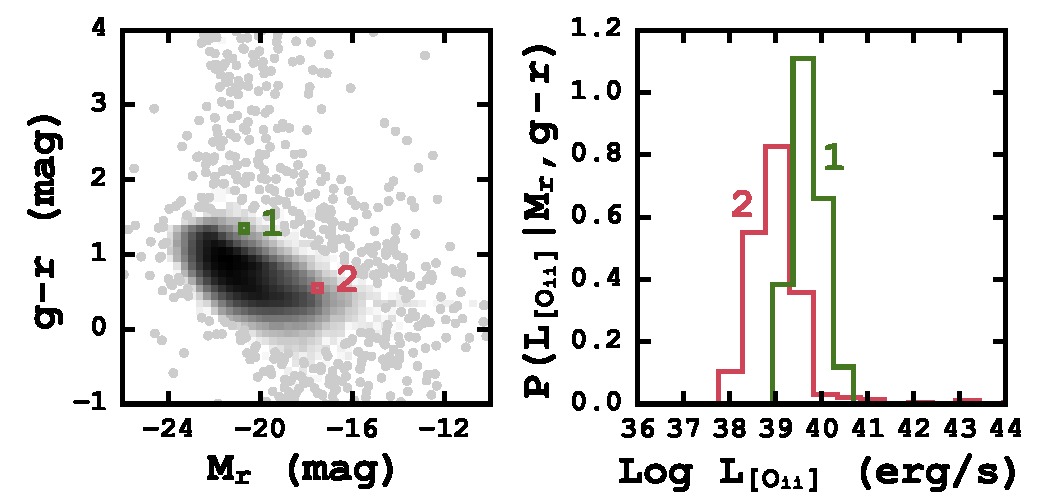
\includegraphics[width=\textwidth]{figures/oii_sdss.pdf} 
	\caption{\textit{Left}: CMD of 503113 $z<0.2$ galaxies take from the SDSS DR12 where the shading scales with the density of points. The two boxes show regions containing potential catalog galaxies. \textit{Right}: Probability histograms of the Log [\ion{O}{ii}] luminosity for the SDSS galaxies located in the two highlighted regions on the right. New [\ion{O}{ii}] luminosity (and subsequently fluxes) are assigned to catalog galaxies from slice sampling the probability histogram.} \label{fig: oii sdss} 
\end{figure*}

The ``Buzzard'' mock galaxy catalogs (R. Wechsler et al., private communication) cover 375.68 \degsq\ between $60 < RA < 90$ and $-61 < DEC < -41$ and are derived from a combination of Sub-halo Abundance Matching (ShAM) and ADDSEDs (Adding Density Dependent Spectral Energy Distributions) tied to an in house n-body cosmological simulation. A brief description of the catalog creation is described as follows. The initial conditions are generated with a second-order Lagrangian perturbation theory using {\tt 2LPTic} \citep{Crocce2006}. Dark matter (DM) n-body simulations are run using {\tt LGadget-2} (a version of {\tt Gadget-2}; \citealt{Springel2005}). The DM halos are identified using the {\tt ROCKSTAR} halo finder \citep{Behroozi2013} which also calculates halo masses and other various parameters. 

Galaxy $M_r$ luminosities are added to the velocity peaks using ShAM \citep{Reddick2013}, and ADDSEDs (Adding Density Dependent Spectral Energy Distributions) assign luminosities in the other bands. A $M_r$-density-SED relation is created using a SDSS training set, and for each mock galaxy the SED of a randomly selected training set galaxy which has a similar $M_r$ and density is assigned. The result is a 398.49 sq. degree mock catalog occupying a $60 \leq RA \leq 90$ and $-40 \leq DEC \leq -61$ portion of the sky. It contains 238 million galaxies with \sdssr\ mag $< 29$ and $z \leq 8.7$.

The catalog information, used in this study, is broken into two large portions. The ``truth'' files contain the characteristics of each individual galaxies, such as right ascension (RA), declination (DEC), redshift (z), observed and rest-frame magnitudes, and many others. The ``halo'' files contain information for individual halos, to which many individual galaxies may belong. This includes five estimations of dynamical mass, RA, DEC, z, three dimensional velocity dispersion, and many others.

However, the catalogs do not include information on emission or absorption lines or estimations of whether the halo is relaxed or not. We supplement the catalogs with this information and describe the method in Section~\ref{sec: oii luminosity} and others.

% \begin{figure}
% 	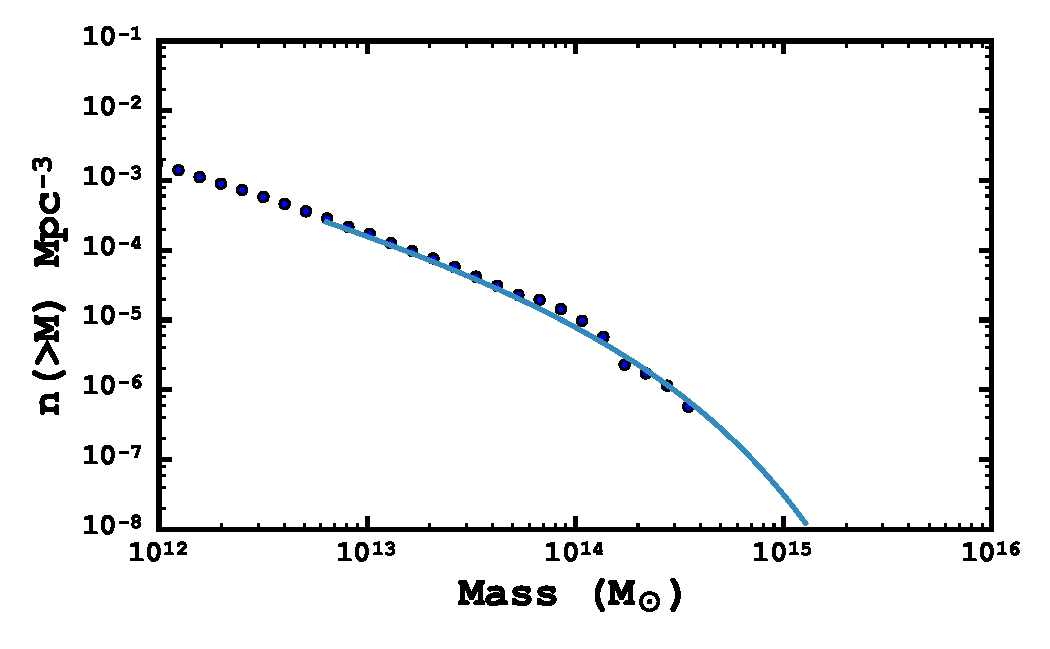
\includegraphics[width=\columnwidth]{figures/hmf.pdf}
% 	\caption{The cumulative MF (from \citealt{Tinker2008}) of halos above $M_{200c}$ at $z=0.1$}
% 	\label{fig: hmf}
% \end{figure}

We investigate the accuracy of the halo mass distribution by comparing the cumulative number density of halos above a mass ($M_{200c}$) threshold to the halo mass function (HMF) of \cite{Tinker2008}. Shown in Figure~\ref{fig: hmf} the HMF is calculated at central redshifts of 0, 0.2, and 0.4 using {\tt HMFcalc} \citep{Murray2013} and compared to galaxies in a redshift window of $\Delta z\pm0.01$. We find a very good agreement between the expected HMF and the observed. 

\subsection{ {\rm[\ion{O}{ii}]} Luminosity}\label{sec: oii luminosity}
The Buzzard ``truth'' catalog does not provide [\ion{O}{ii}] luminosities so we must assign them empirically. We use 503113 galaxies from the SDSS Data Release 12 \citep{Alam2015} from $z = 0.05 - 0.2$, which are selected with no redshift warning, and place each galaxy on a color-magnitude diagram (CMD) of $M_r$ and $g-r$, see Figure~\ref{fig: oii sdss}.

To assign an [\ion{O}{ii}] luminosity to each galaxy in our catalog we place the catalog galaxies on the same CMD and select all SDSS galaxies in a small 2D ($M_r$, $g-r$) bin around the galaxy. We extract all of the SDSS galaxies inside that bin and create a histogram of their [\ion{O}{ii}] luminosities. Using a slice sampling technique \citep{Neal1997} we assign the catalog galaxy an [\ion{O}{ii}] luminosity based on the distribution of SDSS galaxies extracted. For catalog galaxies which are placed on the CMD near no, or very few ($1\leq n<10$) galaxies we assign it zero [\ion{O}{ii}] luminosity or the mean luminosity, respectively.

The right panel of Figure~\ref{fig: oii sdss} shows the CMD of all SDSS galaxies. Two potential catalog galaxies are also placed on the CMD ($M_r, g-r = -17.7,~0.49$ and $M_r, g-r = -21.4,~1.24$) and indicated by two colored boxes. The histograms show in the Figure's left panel shows the probability density histograms of the Log [\ion{O}{ii}] luminosity for the SDSS galaxies in the 2D bin. We sample the distribution and assign each catalog galaxy an [\ion{O}{ii}] luminosity which is then converted into a flux.

\subsection{Mock Observations}\label{sec: observations}
\editorial{Not sure this does a good enough job talking about the two different observations.}
Tentatively slated to start in the spring of 2016, HETDEX will perform blind spectroscopy (R $\sim$ 750 in $3500 - 5500~\AAA$) over two fields along the celestial equator. The 300 \degsq, spring field and 120 \degsq, fall field will have no preselected targets. Using VIRUS on the 10-m Hobby-Eberly Telescope (HET; \citealt{Ramsey1998}) the completed survey is expected to have an overall fill-factor of 1/4.5, meaning that the entire area could be covered with 4.5 dithers of the entire survey. 

The spectral coverage allows for the detection of [\ion{O}{ii}] ($\lambda\lambda 3727-3729~\AAA$ doublet) emitters to $z\sim 0.5$ and Ca H ($\lambda 3968.5~\AAA$) and K ($\lambda 3933.7~\AAA$) absorption features to $z\sim 0.4$. HETDEX is expected to detect sources with continuum brighter than 22 mag in \sdssg, and emission line strengths above $3.5\times10^{-17}$ \ergscm. So we ``observe'' galaxies which meet either the emission line or magnitude requirements. 

\begin{figure} 
	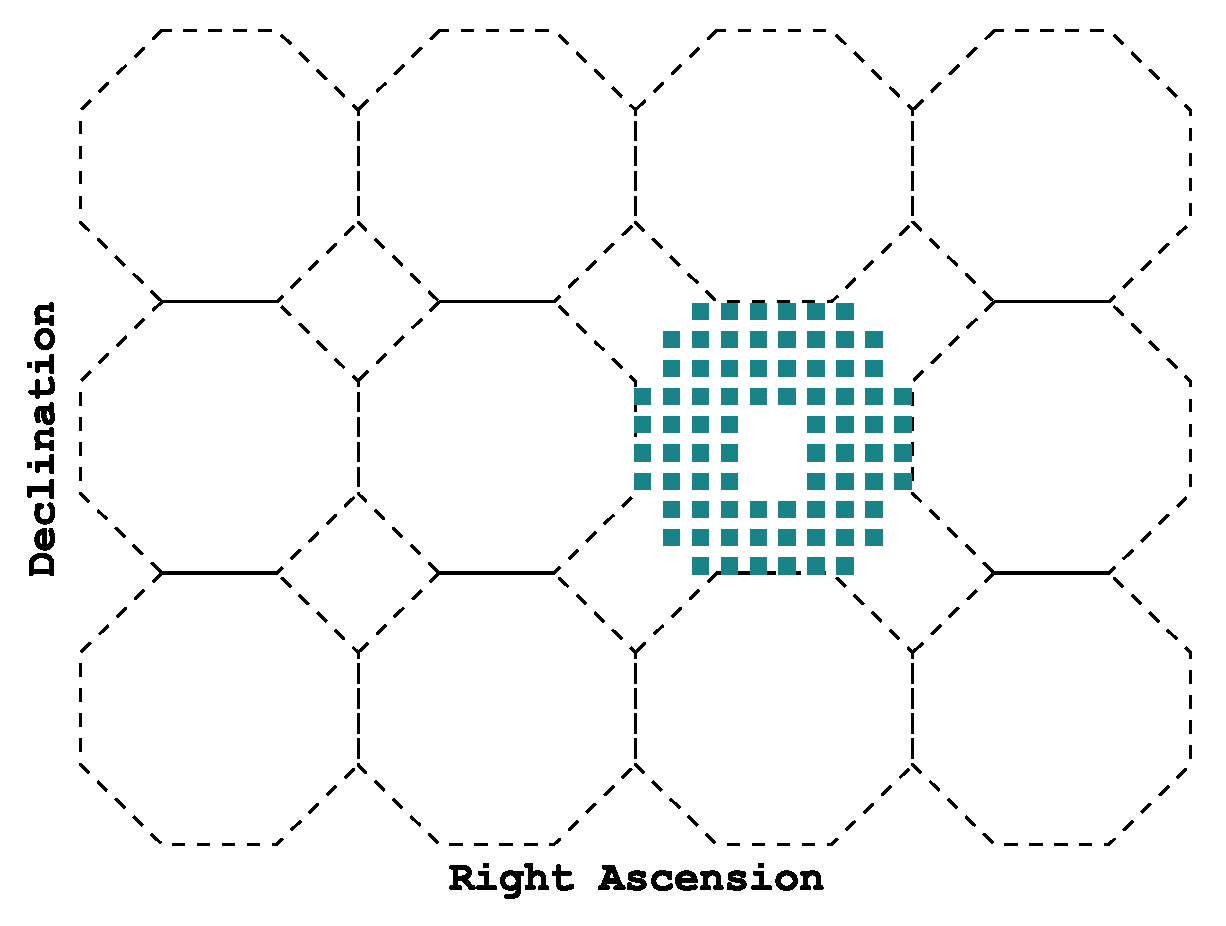
\includegraphics[width=\columnwidth]{figures/f01.pdf} 
	\caption{Representative observation tiling scheme for the HETDEX $16' \times 16'$ pointings. Each colored square is a single VIRUS IFU and the dashed octagons approximate the size of a single observation. See the text for more details.} \label{fig: ifu layout} 
\end{figure}

In this work we consider two separate observation cases. The first are targeted observations where we select each galaxy cluster and ``observe'' each galaxy within $8'$ of the center. The second is a survey case where observations which are blind to the positions of the clusters are conducted. In both cases, our ``observations'' consist of placing masks down onto the Buzzard ``truth'' catalogs and selecting all, $z< 0.5$ also meeting sensitivity limits, galaxies which lie underneath. Each mask is created to accurately reproduce the HETDEX IFU pattern, see Figure~\ref{fig: ifu layout}. The pattern consists of 78 IFUs, which are comprised of 448 optical fibers subtending a $50'' \times 50''$ region on the sky \citep{Kelz2014}. The inter-IFU spacing is also $50''$ spanning a total area of $16'\times 16'$ on the sky. 

The individual IFUs have a fill-factor of 1/3, which will be completely filled with three dithers of the telescope at each pointing. This means that when selecting galaxies from the Buzzard catalog we assume an observation for all galaxies laying within a colored, IFU square in Figure~\ref{fig: ifu layout}. \editorial{This should be updated with the fiber collisions.} Galaxies which lie between the IFUs are missed, as well as the galaxies which lie between the pointings, as there is no overlap between one pointing and the next. To cover the 375.67 \degsq\ field of the Buzzard catalog we require 5370 pointings where 0.015 \degsq\ of each pointing is covered by an IFU. The total area of the sky covered by an IFU is 80.80 \degsq\ which gives a filling factor of 1/4.65 slight decreased from the expected filling factor of 1/4.5. 

\section{Recovery of Parameters}\label{sec:recovery}
 In the following sections, we outline the methods we use to derive the dynamical properties of the galaxy clusters in our sample. This is not meant to be an exhaustive study of the different methods used to recover these parameters. The following is, in many cases, a subset of the available methods to derive any single parameter. The specific choice of method may improve or diminish the accuracy of the recovered parameter, but the methods chosen were to facilitate comparison with observational studies. 

\subsection{Cluster Redshift}
The accurate determination of the cluster redshift ($z_c$) is crucial to the reliability of all following measurements. An incorrect cluster redshift introduces errors into the measured line-of-sight velocity (LOSV) and corresponding dispersion, which, in turn, contributes to errors associated with dynamical mass and radius. 

In simple terms, the cluster redshift is the mean of the redshifts of all galaxies associated with the cluster. However, because the standard mean can be quite sensitive to outliers or otherwise contaminated data, we require a more resistant statistic, and turn to the biweight location estimator \citep{Beers1990} which provides improved performance. 

\subsection{Line-of-Sight Velocity Dispersion}\label{sec: LOSVD}
We first calculate the line-of-sight velocity (LOSV) to each galaxy, where
\begin{equation}
	LOSV = c\frac{z - z_c}{1+z_c}
\end{equation}
and $c$ is the speed of light in \kms, $z$ is the redshift of the individual galaxy, and $z_c$ is the overall cluster redshift described in the previous section.

The line-of-sight velocity dispersion (LOSVD) is calculated using a method of maximum likelihood following \cite{Walker2006}. We maximize the probability function 
\begin{equation}
  \label{eq: jointGaussian}
p(\{v_1, ..., v_N\})=\displaystyle\prod_{i=1}^{N}\frac{1}{\sqrt{2\pi(\sigma_i^2+\sigma_p^2)}}\exp\biggl[-\frac{1}{2}\frac{(v_i-\langle u \rangle)^2}{(\sigma_i^2+\sigma_p^2)}\biggr]
\end{equation}
where $\sigma_p$, $\langle\mu\rangle$, and $\sigma_i$ is the LOSVD, the average radial velocity and the error on the individual LOSVs respectively. Using a Monte Carlo Markov Chain (MCMC) sampler ({\tt emcee}); \citealt{Foreman-Mackey2013}), we draw twenty thousand samples from the posterior probability distribution. Simple priors, $\langle\mu\rangle$ lies between the maximum and minimum LOSV and $0< \sigma_p$ \editorial{check}, are used. When the full distribution of LOSVDs are not used, the final LOSVD is quoted as the median value of the posterior probability distribution with 68\% error bars defined as the 16th and 84th percentiles of the same distribution.

In principle, a single statistic such as the biweight scale estimator or the gapper estimator (both from \citealt{Beers1990}) with many bootstrap resamplings could be used to construct a distribution of $\sigma_p$. In simple tests where the values of both $\sigma_p$ and $\langle\mu\rangle$ are known. The 68\% error bars derived from the MCMC method give slightly better results with the true LOSVD value bracketed by the error bars in $\sim68\%$ of the cases versus $\sim57\%$ with bootstrapping and a single statistic. In addition, we prefer the maximum likelihood method for its straight forward treatment of the errors in the LOSV measurements.

\subsection{Dynamical Mass}\label{sec: mass}
Recently, the relationship between the LOSVD and dynamical mass has been the focus of several studies \citeeg{Evrard2008, Saro2013, Sifon2013, VanderBurg2014}, and a best fitting relationship for the mass enclosed by $r_{200c}$ of the form
\begin{equation}\label{eq:power law}
	M_{200c} = \frac{10^{15}}{h(z)} \bigg{(}\frac{\sigma_{1D}}{A_{1D}} \bigg{)}^{1/\alpha} \Msol
\end{equation}
with $A_{1D} = 1177 \pm 4.2$ \kms\ (\citealt{Munari2013}; referred to as $\sigma_{15}$ in \citealt{Evrard2008} and other works), $\alpha = 1/3$, $h(z) = H(z)/100$, and $\sigma_{1D}$ is the LOSVD of the velocity tracers (dark matter particles, subhalos or galaxies). 

A growing body of work suggests that there is a significant difference in the observed LOSVD depending on the velocity tracers used. Specifically, while there is little difference between using galaxies and their host DM subhalos, there is a significant over estimation of the LOSVD when using galaxies/subhalos compared to DM particles \citep{Munari2013}. We follow other works \citeeg{Kirk2015, Sifon2015a} using the scaling relation, given in Equation~\ref{eq:power law} from \cite{Munari2013} to facilitate comparisons with other observational studies. 
% \editorial{This all needs to be stripped out and reworked.}
% The choice $A_{1D}$ and $\alpha$ varies between studies \citeeg{Munari2013, VanderBurg2014} and should be calibrated on a individual basis. To do this, we randomly select 47494, $z<0.5$ clusters composed of 36000 $10^{13}$, 6000 $10^{14}$ and two $10^{15}~\Msol$ halos. We perform a linear fit to the $\sigma_{1D}-M_{200}$ values allowing both $A_{1D}$ and $\alpha$ to vary. We find best fitting parameters of $A_{1D} = 1117.9~\kms$ and $\alpha = 0.3297$, both of which are very near the values from \cite{Evrard2008} of $A_{1D} = 1082.9 \pm 4.0~\kms$ and $\alpha = 0.3361$. Therefore, we chose to adopt the parameters from \cite{Evrard2008} to better facilitate with other simulations \citeeg{Old2014}, and observational studies \citeeg{Brodwin2010}.

\subsection{Dynamical Mass Corrections}
In this section we use two methods to predict the mass of a cluster based on other observables. Often the cluster mass is estimated based on a single observable, X-ray temperature, velocity dispersion, richness and others. Here we combine many observables to attempt to correct the mass inferred solely from the velocity dispersion. The first method is traditional probability based where we marginalize over a series of observables to find the most probable mass. The second is based on a machine learning (ML) algorithm which attempts to ``learn'' the relationship between the observables and the desired output, the mass. Both of these methods are examples of supervised learning algorithms where the relationship between the observable (known) parameters and the target parameter (the mass) are both known.

As with any predictive analysis it is important to test the model on data that the model has not seen before. In this section we take all of the observed clusters, our full sample, split them, and generate a training and testing set. The data is randomly split 70\% training and 30\% testing. We follow the ML convention and refer to the individual clusters in each set as a ``sample'', and the parameters associated with the cluster ($z$, LOSVD, mass, etc.) as ``features''.  

\subsubsection{Probability Based}\label{sec:probability method}
We begin with the training sample. After selecting the desired features $\vec{x} = \{\sigma, z, ...\}$ we make the joint probability between the true cluster mass (M) and $\vec{x}$. Because $\vec{x}$ can be multidimensional, we rely on the corner plot to visualize the relationship between all of the training features. Figure~\ref{fig: probability corner} shows all of the one (marginalized probability) and two (joint probability) dimensional projections of the posterior probability distributions of the features of the training data.

\begin{figure} 
	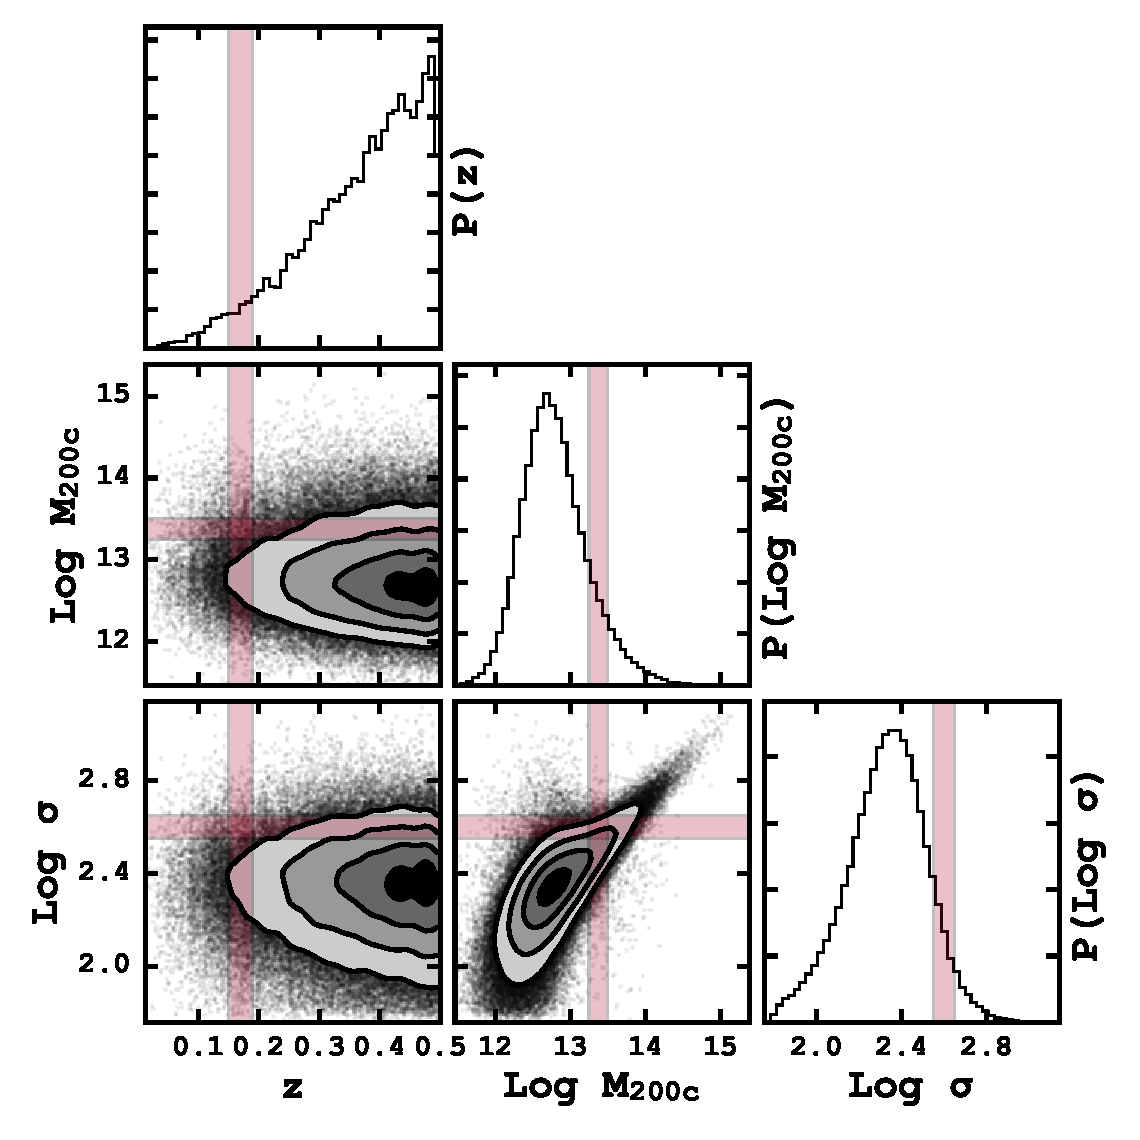
\includegraphics[width=\columnwidth]{figures/cornertest.pdf} 
	\caption{Corner plot of the \emph{training} data with features $\sigma$ and $z$. The corner plots shows all of the one and two dimensional posterior probability distributions used to determine the correct cluster mass. The colored rectangles show the slices needed to create a conditional probability distribution of the mass, $P(M|\vec{x})$. See text for a complete description. } \label{fig: probability corner} 
\end{figure}

The conditional probability of the mass $P(M|\vec{x}= \{ x_1,x_2,...\})$ is determined by taking a slice through the joint probability distributions in bins centered on the desired value. The slices show by the colored bars in Figure~\ref{fig: probability corner} are centered on $\sigma = 500$ \kms and $z=0.17$. The distribution of mass contained in the three dimensional bin given by the intersection of these slices is $P(M|\vec{x} = \{ \sigma=500 \kms,z=0.17\})$.

\begin{figure*}
	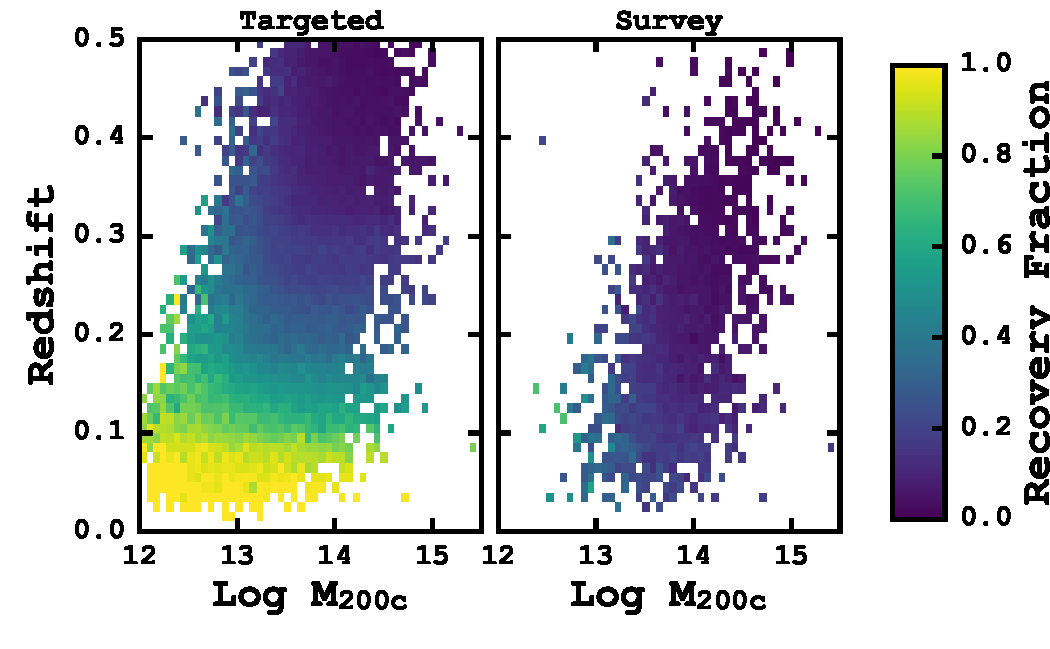
\includegraphics[width=0.8\textwidth]{figures/recovery.pdf} 
	\caption{Recovery fractions ($N_{obs}/N_{True}$) of cluster member galaxies as a function of redshift and mass for the targeted and survey observing strategies. The solide lines are the median values and the shaded regions represent the 68\% scatter. The significant decline in galaxies observed with the survey strategy is due to gaps in the VIRUS IFU.} \label{fig: recovery} 
\end{figure*}

For the clusters making up the \emph{test} sample the mass is unknown (it is what we are trying to predict) but the other features are known. To determine the mass probability distribution of a test cluster, $P(M)$ we combine the conditional probability distribution, $P(M|\vec{x})$, created previously with the probability distribution of $\sigma$ through Equation~\ref{eq: Pm}.
\begin{equation}\label{eq: Pm}
	P(M) = \int P(M|\vec{x}) P(\sigma) d\sigma
\end{equation}
The expected mass is determined by integrating the mass probability, $P(M)$ over all mass. This becomes our ``predicted'' mass, $\langle M\rangle$.
\begin{equation}\label{eq: expected mass}
	\langle M\rangle = \int M^\prime P(M^\prime)dM^\prime
\end{equation}
The confidence interval associated with this prediction can be estimated two ways. First, by calculating the variance about the expected mass through
\begin{equation}\label{eq: variance}
	V = \int (M^\prime - \langle M\rangle)^2 P(M^\prime)dM^\prime
\end{equation}
or by drawing many samples from $P(M)$ and calculating the values at the 16th and 84th percentile. In practice we find that both methods produce similar results for a large number of trials. Therefore, we quote predicted masses as the most probable mass given by Equation~\ref{eq: expected mass} and associated 68\% error estimated through Equation~\ref{eq: variance}.

\subsubsection{Machine Learning Based}\label{sec:machine learning method}
The estimation in this section relies on a ML technique known as an ensemble method, where many estimators are created by a single learning method with the goal of improved generalization and robustness compared to a single estimation. Ensemble methods come in two general flavors. Averaging methods average (hence the name) the estimators to produce a single prediction. Boosting estimators build estimates sequentially by attempting to address poor performing estimators in each previous step, hence ``boosting'' the predictive power.

Here we use an averaging ensemble learning method known as a forest of randomized decision trees often shorten to just random forest (RF). Decision trees can be visualized a flow chart where forks are the branches of the tree. The path along the tree is decided by the values of the feature at each branch. RF estimators use a random subset of the training set at each fork to decide which path should be followed. The final prediction is then the average of all the trees. We use RF regression methods as implemented in {\tt Scikit-Learn} \citep{Pedregosa2012}.

Any uncertainties quoted by this method are prediction intervals not confidence intervals. A prediction interval is an estimate of the interval encompassing future observations, with a certain probability. And, unlike confidence intervals, which describe certainties on the different moments of a population, a prediction interval is unique to each prediction. In many regresson analyses, such as linear fitting, the prediction intervals are based on underlying assumptions of normally distributed residuals. However, RF estimators do not have any such assumptions and require special treatment.

The prediction intervals here are based on the general method of quantile regression forests \citep{Meinshausen2006}. The general idea is that all response variables are recorded, not just the mean. Then the prediction can be returned as the full conditional probability distribution of all responses, which allows us to generate the prediction intervals. The 68\% prediction interval is determined by calculating the 16th and 84th percentile of the full conditional probability distribution. \editorial{I am going to change this to just the std of the distribution. I need the errorbars to be sysmetric to make the fitting routine easy later on.}

\section{RESULTS}\label{sec:results}
Here we explore the cluster member recovery rate and mass estimates for the two observing strategies. We discuss the accuracy of dynamical mass derived from both the scaling relation (see Equation \ref{eq:power law}) and through the probability and ML methods.

\subsection{Recovery of Cluster Members}
As discussed in Section \ref{sec: observations} the observational constraints place limits on the total number fo clusters member galaxies expected to be recovered. Knowing these limits will provide important information for potential future follow up or targeted observations. 

Figure \ref{fig: recovery} shows the recovery fraction of member galaxies, the number of observed galaxies divided by the number of actual galaxies ($N_{obs}/N_{True}$), as function of both redshift and cluster mass. It is important to note that if few than five member galaxies are observed the cluster is not considered detected, and is excluded from this figure. As expected, the targeted observing strategy where the individual clusters are targeted through several dithers to ensure near complete coverage, performs significantly better than the survey observing strategy across all redshifts and cluster masses. 

For the clusters recovered as a function of redshift, there are two effects at work. The decrease in recovery fraction with increasing redshift is a magnitude effect. If, instead of being limited to 22 mag in \sdssg apparent, the observations where limited by absolute magnitude, the sharp downward trend disappears. The second key feature is the strong decline in clusters recovered from survey observations. This is due to gaps in the VIRUS IFU. The median recovery fraction in survey observations is almost exactly 4.5 times less than the targeted median recovery fraction. As the total filling factor of the survey increases the two lines will converge.

The recovery rate as a function of cluster mass, right panel of Figure \ref{fig: recovery}, shows that of the the low mass clusters we detect ($N_{obs} >5$), observe the majority of the galaxies. This also shows a rapid decrease in the detection fraction, which can again be explained by considering absolute magnitudes instead of apparent magnitudes. Just as before, if the survey was limited by absolute magnitude, we find a much more consistent detection fraction.

\subsection{Mass estimates}
In this section we discuss the how accurately we are able to reproduce the true cluster mass from a set of observations. We report on two methods the probability based approach (Section \ref{sec:probability method}) and the ML based method (Section \ref{sec:machine learning method}). For each method we consider both targeted and HETDEX-like observing strategies.

In both figures, we include the cluster masses recovered through the power law scaling relation given in Equation \ref{eq:power law} for both the targeted and survey observations. It should serve as baseline to compare the probability based and ML cluster mass recovery methods. And, while there are many possible metrics to evaluate performance, we compute two: the median absolute error (MAE) and the root mean squared error (RMSE). Both metrics evaluate how closely the ensemble of predicted cluster masses are to the true cluster masses, and in both cases lower numbers are better.   

Just because a predicted cluster mass may not exactly match the true value does not mean it is a bad prediction. In addition to the MAE and RMSE, we also report the fraction of predictions where the the true cluster mass is contained within the 68\% confidence or prediction intervals (see Sections \ref{sec:probability method} and \ref{sec:machine learning method}). 

The cluster masses predicted by Equation \ref{eq:power law} gives the following results. The MAE is 0.263 dex and for both the targeted and survey observations. The RMSE is 0.396 dex and 0.394 dex for the targeted and survey observations respectively. This scatter in recovered masses can be attributed to both physical and numerical effects. As the cluster mass increases, clusters become more virialized and contain many individual galaxies. The presence of any in-falling matter onto lower mass clusters can introduce a significant amount of substructure, which can increase the observed LOSVD increasing the predicted mass. Also, as the number of cluster galaxies decreases the LOSVD PDF is poorly sampled leading to poorly recovered cluster masses due to numerical effects. The masses presented here are recovered using the best possible conditions, where we have perfect knowledge of the cluster membership. In reality, the mass recovery levels presented in this section represent an upper bound (the best) on the accuracy achievable through this method. \editorial{\cite{Ntampaka2015} does have a discussion about how well they do with contaminated galaxy catalogs. We could do something similar and have a similar discussion, but I'm not sure it is worth it. Should be simple enough to do with the targeted catalog, but with the HETDEX catalog it would be pretty bad IMO. We should also talk about how often the true mass lies within the error bars. Many of them are going to be with the 68\% range, but we can drop the error estimates to $0.5\sigma$ if that actually means anything} 

\begin{table*}
\centering
\caption{Summary of the errors associated with the Targeted and Survey observation strategies, as an ensemble of predictions. See the text for discussion about the MAE and RMSE. Overlap is the percentage of clusters where the true cluster mass is bracketed by the prediction intervals of the predicted mass. See Sections \ref{sec:probability method} and \ref{sec:machine learning method} for a discussion on prediction intervals.}
\begin{tabular}{cccccccc}
	%\hline
	&& \multic{3}{Targeted} & \multic{3}{Survey} \\
	\cline{3-5} \cline{6-8}
	& Input Features & MAE & RMSE & Overlap & MAE & RMSE & Overlap \\
	& & (dex) & (dex) & (\%) & (dex) & (dex) & (\%) \\
	\hline
	\rottext{4}{Prob Based} & Power Law & 0.263 & 0.396 & --- & 0.263 & 0.393 & --- \\
	&$\sigma$ & 0.220 & 0.335 & --- & 0.222 & 0.329 & --- \\
	&$\sigma, z$ & 0.189 & 0.286 & --- & 0.194 & 0.278 & --- \\
	&$\sigma, z, N_{gal}$ & 0.129 & 0.207 & --- & 0.140 & 0.222 & --- \\

	\hline
	\rottext{4}{ML Based} & Power Law & 0.263 & 0.396 & --- & 0.263 & 0.393 & --- \\
	&$\sigma$ & 0.246 & 0.361 & --- & 0.238 & 0.344 & --- \\
	&$\sigma, z$ & 0.193 & 0.285 & --- & 0.171 & 0.260 & --- \\
	&$\sigma, z, N_{gal}$ & 0.117 & 0.193 & --- & 0.093 & 0.179 & --- \\

	\hline
\end{tabular}
\label{tbl:mass comparisons}
\end{table*}

The MAE and RMSE associated with the ensemble of predictions are summarized in Table \ref{tbl:mass comparisons}. As expected, we find that both the probability based and ML based methods out perform the standard power law based methods for both the targeted and survey observations. We also find that the ML based method produces lower ensemble error for both the observation strategies when compared to the probability based method, although the MAE and RMSE are reduced by only $\sim0.01$ dex. \editorial{here is where we would talk about cross validation on the errors.} 

In both Figures \ref{fig:Probability comparison} and \ref{fig: ML comparison}, we show the predicted versus true cluster masses for each of the two observing strategries. In each panel the solid black line is the 1:1 relationship, the solid colored line is the median recovered mass for the targeted observing, and the colored, dashed line is the median recovered mass for the HETDEX-like observations. The shaded regions are the 68\% scatter around the median values (the 16\% and 84\% quartiles). The lower panels show the fractional cluster mass error: 
\begin{equation}\label{eq: fractional error}
	\epsilon = (M_{pred} - M)/M
\end{equation}
where $M_{pred}$ is the predicted cluster mass and $M$ is the true cluster mass.

In both figures we successively add additional information to further contrain the true cluster masses which subsequently reduces the error associated with the ensemble of predictions (see Table \ref{tbl:mass comparisons}). The power law derived masses, using the single (not including the cosmological parameters) free parameter, $\sigma$ (the LOSVD), over estimates the predicted cluster mass at all masses. Both the probability and ML methods over predict the mass of low mass clusters and under predict the mass of the higher mass clusters. When the redshift information is also added, the amount of this over and under prediction is lessened but the cross over point, remains roughly consistent at $\sim10^{14}$ \msol. Additionally, the number of galaxies observed, $N_{gal}$, further reduces the MAE and RMSE on the predictions but also lowers the cross over point to $\sim10^{13.5}$ \msol.

\begin{figure*} 
	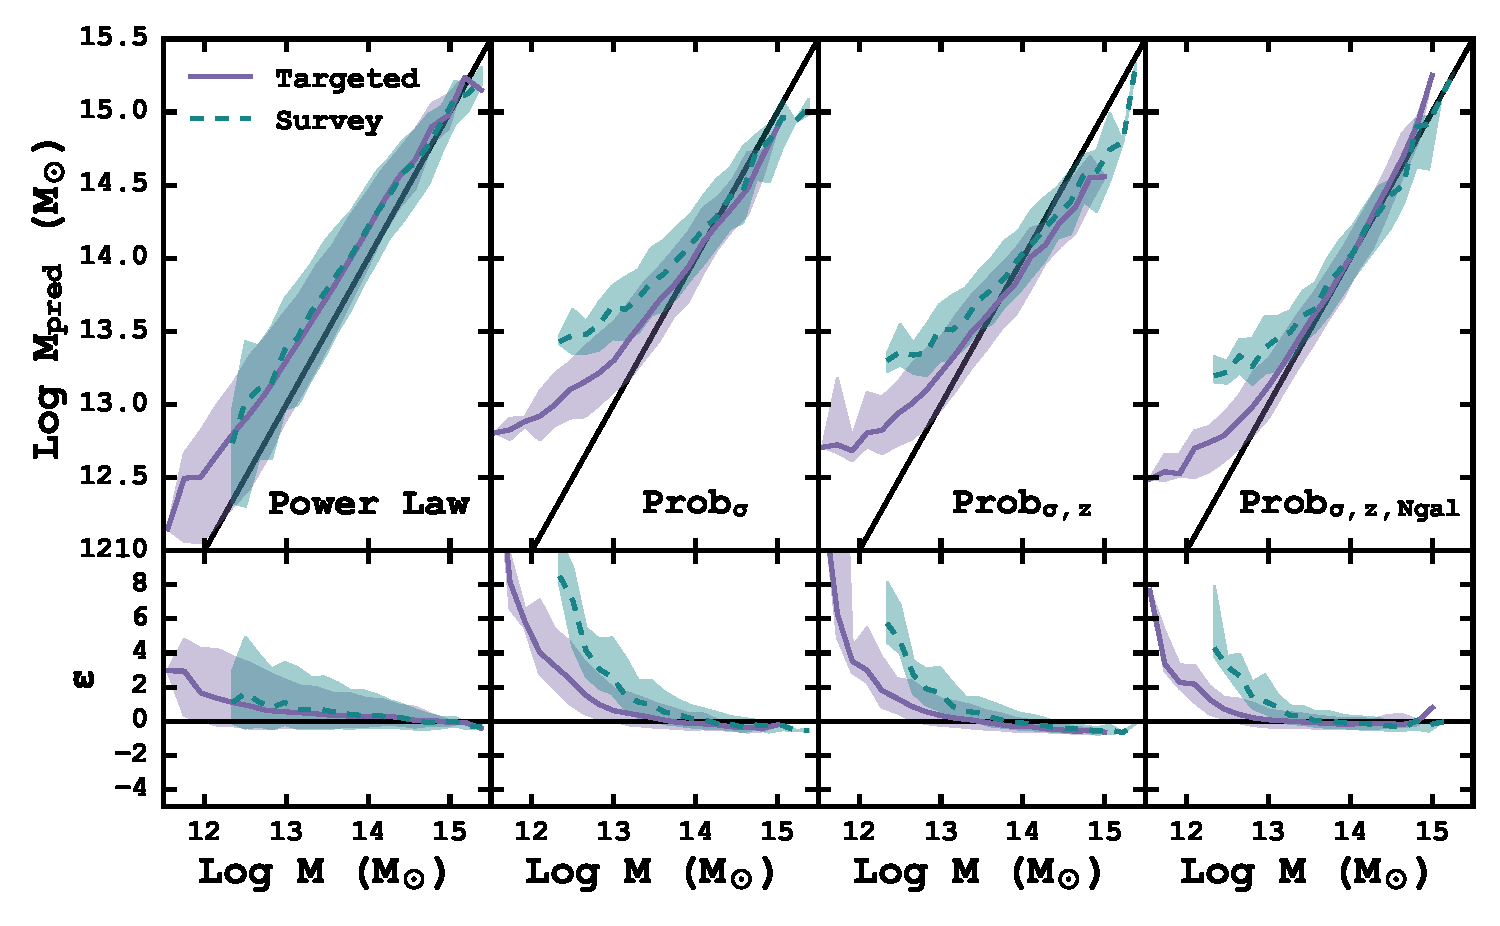
\includegraphics[width=\textwidth]{figures/Probcomparison.pdf} 
	\caption{Mass predictions for the power law scaling relation (Equation~\ref{eq:power law}) and the probability based technique with different input features as a function of true cluster mass. The bottom row of panels shows the fractional error (Equation~\ref{eq: fractional error}) also as a function of true cluster mass. The solid black line shows the 1:1 relation. The solid, colored line is the median predicted mass for the targeted observing, and the colored, dashed line is the median recovered mass for the HETDEX-like observations. The shaded regions represent the 68\% scatter around the median values.} \label{fig:Probability comparison} 
\end{figure*}

\editorial{Need to talk about the cluster rotations to fill out the survey data. Otherwise there aren't that many clusters detected.} 

\begin{figure*} 
	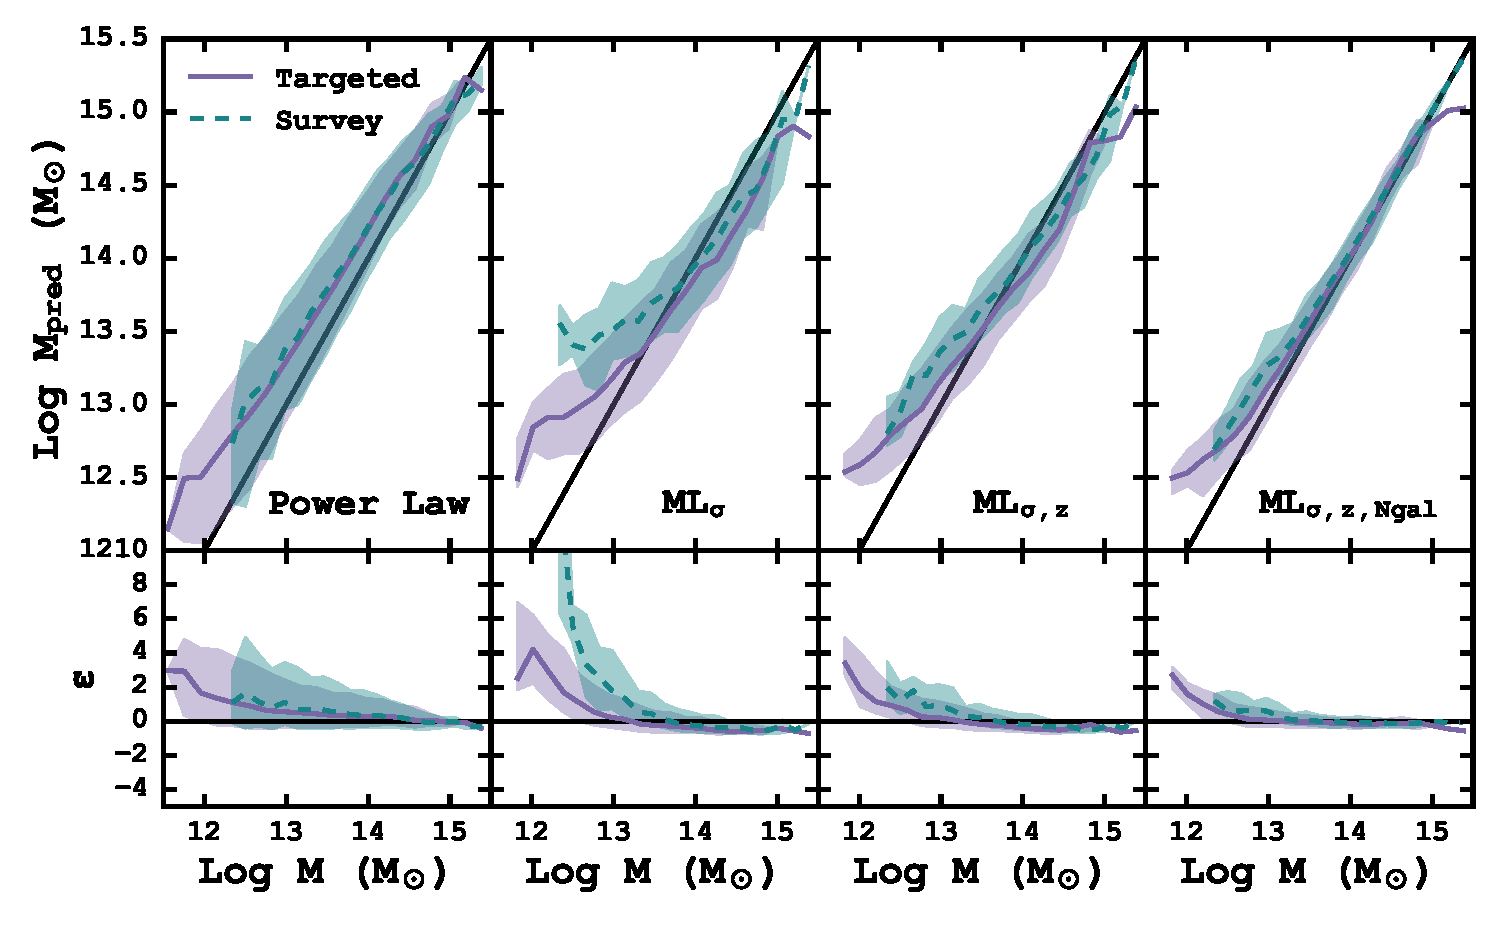
\includegraphics[width=\textwidth]{figures/MLcomparison.pdf} 
	\caption{Mass predictions for the power law scaling relation (Equation~\ref{eq:power law}) and the ML based technique with different input features as a function of true cluster mass. The bottom row of panels shows the fractional error (Equation~\ref{eq: fractional error}) also as a function of true cluster mass. The solid black line shows the 1:1 relation. The solid, colored line is the median predicted mass for the targeted observing, and the colored, dashed line is the median recovered mass for the HETDEX-like observations. The shaded regions represent the 68\% scatter around the median values.} \label{fig: ML comparison} 
\end{figure*}

% \editorial{It doesn't look like you can use the targeted training sample to train the survey data. If you do, it either does worse or about the same if you didn't use any training at all. After looking at it, you do have to use the survey training data to get good results about 0.13 dex MAE
% }

\section{HETDEX as a Galaxy Cluster Survey}\label{sec:discussion}

\subsection{Extendability to Other Surveys}
Large-scale optical surveys (\eg, DES and LSST) expect to detect hundreds of thousands of galaxy clusters at $z < 1$. Because they are photometric, a major challenge for these surveys is relating a cluster observable to the total dark-matter mass. One promising mass estimator is the optical richness \citeeg{Abell1958}. Specifically, here, we use $\lambda$, the weighted number of galaxies within a scale aperture \citeeg{Rozo2011} as calculated by the redMapper algorithm \citep{Rykoff2012}. Previous works \citeeg{Rozo2010} show that the richness correlates strongly with cluster mass on the average, but the absolute mass scale of the optical richness mass estimator and the scatter in cluster mass at fixed optical richness are imprecisely known \citep{Rykoff2012}. These systematics remain the major source of uncertainty in deriving cosmological constraints from cluster abundances and must be measured using independent methods to realize the full potential of these surveys.

\begin{figure} 
	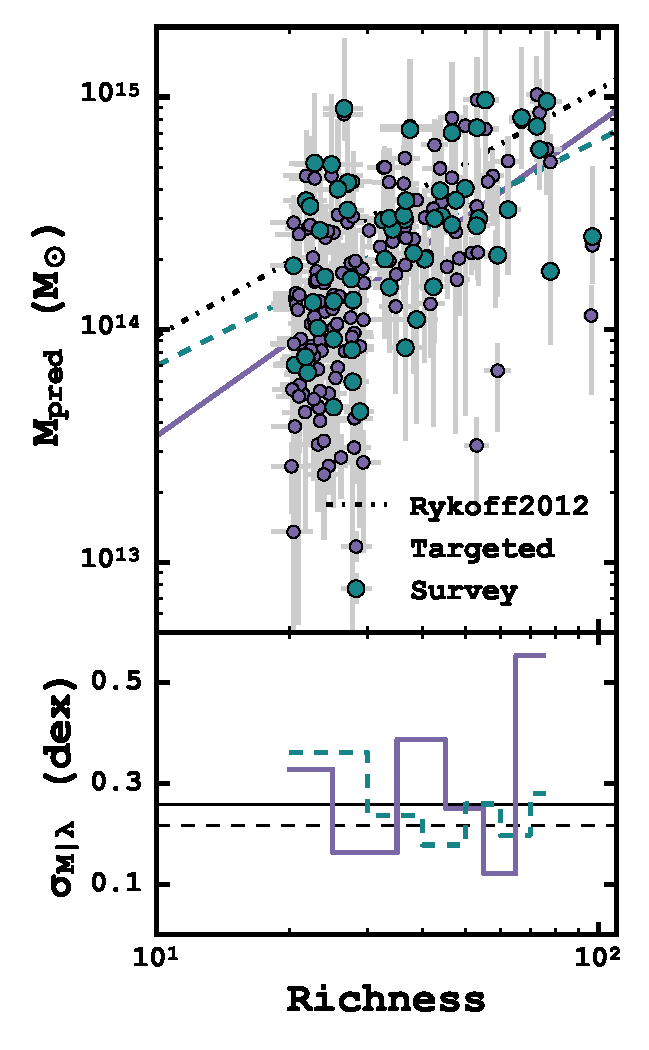
\includegraphics[width=\columnwidth]{figures/massRichness_targeted.pdf} 
	\caption{The optical richness, $\lambda$, versus the predicted cluster mass. The purple and blue points represent clusters with targeted and survey detections respectively. Error bars show $1\sigma$ prediction interval. The solid and dashed lines are fits to either the targeted or survey sets. } \label{fig:mass richness} 
\end{figure}

We leverage the large spectroscopic dataset of HETDEX to estimate its ability to constrain the scatter and absolute scale of the richness-mass relationship. We begin by cross matching both the targeted and survey observations with a redMapper catalog. The redMapper catalog is limited to $\lambda >= 20$, or at least twenty object assigned to each cluster. With the targeted and survey observations, we observe 138 and 58 clusters respectively. 

Figure \ref{fig:mass richness} shows the optical richness, $\lambda$, versus the predicted cluster mass. The cluster masses are the $ML_{\sigma, z, N_{gal}}$ based and correspond to the correct observation strategy. The error bars represent the $1\sigma$ prediction intervals for each cluster mass. The solid and dashed lines are fits to the targeted and survey datasets. For comparison, the richness-mass relations from \cite{Rykoff2012} (their equation B5) is shown as a dash-dotted line.

To generate the best fitting lines we follow the general procedure of \cite{Hogg2010}, by defining an objective function and then minimizing the loss. Our loss function is
\begin{equation}
	\mathrm{ln}L= \frac{-1}{2} \bigg{(} \sum^N_{i=1}\frac{[y_i - mx_i - b]^2}{\sigma_{yi}} + \sum^N_{i=1}\frac{[y_i - mx_i - b]^2}{\sigma_{xi}} \bigg{)}
\end{equation} 
where we have taken into account the uncertainties in both the richness and predicted cluster mass. We again rely on MCMC samples to sample the posterior probability distribution. The best fitting slope and intercept are quoted as the median value of the posterior probability distribution with 68\% error bars defined as the 16th and 84th percentiles of the same distribution.

Following the notation of \cite{Rykoff2012} we find a best-fitting relation for the targeted observations as
\begin{equation}
	ln\bigg{(}\frac{M_{200c}}{h_{70}^{-1} 10^{14}\Msol}\bigg{)} = 1\pm0.13 + 1.34\pm0.17 ln\bigg{(}\frac{\lambda}{60}\bigg{)} \nonumber
\end{equation}
and the survey observations as
\begin{equation}
	ln\bigg{(}\frac{M_{200c}}{h_{70}^{-1} 10^{14}\Msol}\bigg{)} = 1.02\pm0.13 + 0.96\pm0.22 ln\bigg{(}\frac{\lambda}{60}\bigg{)} \nonumber
\end{equation}

The bottom panel of Figure \ref{fig:mass richness} shows the scatter in cluster masses at fixed richness, $\sigma_{M|\lambda}$. The solid and dashed lines represent the targeted and survey observations respectively, and have been offset from one another for clarity. The cluster masses are binned in increasing ten richness intervals ($20-30$, $30-40$, etc.). The two horizontal lines show the mean scatter of 0.26 dex for the targeted observations and 0.21 dex for the survey observations. While not shown in the figure, we find a mean scatter of 0.27 dex if we replace $M_{pred}$ with the true cluster mass for the clusters identified with targeted observations.  

We expect the targeted observations to have more scatter because the survey observations are 

Much like the MAE and RMSE associated with the cluster mass recovery, comparing the individual $\sigma_{M|\lambda}$ values directly is incorrect. When comparing only the clusters with observations in both the targeted and survey stratigies we 
	
%Applying my current work to a large photometric survey such as those mentioned above is the logical next step. For example, the HETDEX observations overlap with the DES area and SDSS Stripe 82 which provides a wealth of external data. Using preexisting datasets, the observations from HETDEX, or through dedicated followup spectroscopic observations, I will be able to measure the absolute mass scale of the richness estimator and measure the scatter of the richness-mass relation, $\sigma_{M|\lambda}$. An accurate measure of this scatter can lead to a decrease on the error bar on cosmological measures ($\sigma_8$ and $\Omega_M$) by as much as 50\% \citep{Rozo2010}. An absolute calibration of the richness-mass relation will provide a much needed tool for future imaging surveys which will identify clusters to $z=1$ and beyond.

\subsection{Potential Improvements}
\editorial{The potential improvements are really three fold. We know that the observing won't cover all of the sky. So we can simply tile more and try to get more clusters. We can observe deeper. I'm not sure the current exposure times (they are in an email that I sent to casey) but if we can extend them, then we can get further down the IMF and try to build up some of the clusters that are really more like groups than anything else. The last thing we can do is to attempt to  build better models to make better predictions on the masses. That might be something like the study that \cite{Acquaviva2016} did with the stellar metallicities. Or we'll need something else that I haven't thought of just yet. The other idea is to come up with some sort of cheat sheet for HETDEX. Basically, a if you detect such and such type of galaxy in the survey model then you should go back and try to follow it up with targeted observations. It might be good to talk about the recovery fraction between the two surveys above. Like... if there are 30 cluster members then we should detect the cluster in both surveys.}

Lorem ipsum dolor sit amet, consectetur adipisicing elit, sed do eiusmod tempor incididunt ut labore et dolore magna aliqua. Ut enim ad minim veniam, quis nostrud exercitation ullamco laboris nisi ut aliquip ex ea commodo consequat. Duis aute irure dolor in reprehenderit in voluptate velit esse cillum dolore eu fugiat nulla pariatur. Excepteur sint occaecat cupidatat non proident, sunt in culpa qui officia deserunt mollit anim id est laborum.


\section{SUMMARY}\label{sec:summary}
Lorem ipsum dolor sit amet, consectetur adipisicing elit, sed do eiusmod tempor incididunt ut labore et dolore magna aliqua. Ut enim ad minim veniam, quis nostrud exercitation ullamco laboris nisi ut aliquip ex ea commodo consequat. Duis aute irure dolor in reprehenderit in voluptate velit esse cillum dolore eu fugiat nulla pariatur. Excepteur sint occaecat cupidatat non proident, sunt in culpa qui officia deserunt mollit anim id est laborum.

Our main conclusions are the following:
\begin{enumerate}
	\item Lorem ipsum dolor sit amet, consectetur adipisicing elit, sed do eiusmod tempor incididunt ut labore et dolore magna aliqua. Ut enim ad minim veniam, quis nostrud exercitation ullamco laboris nisi ut aliquip ex ea commodo consequat. Duis aute irure dolor in reprehenderit in voluptate velit esse cillum dolore eu fugiat nulla pariatur. Excepteur sint occaecat cupidatat non proident, sunt in culpa qui officia deserunt mollit anim id est laborum.
	\item Lorem ipsum dolor sit amet, consectetur adipisicing elit, sed do eiusmod tempor incididunt ut labore et dolore magna aliqua. Ut enim ad minim veniam, quis nostrud exercitation ullamco laboris nisi ut aliquip ex ea commodo consequat. Duis aute irure dolor in reprehenderit in voluptate velit esse cillum dolore eu fugiat nulla pariatur. Excepteur sint occaecat cupidatat non proident, sunt in culpa qui officia deserunt mollit anim id est laborum.
	\item Lorem ipsum dolor sit amet, consectetur adipisicing elit, sed do eiusmod tempor incididunt ut labore et dolore magna aliqua. Ut enim ad minim veniam, quis nostrud exercitation ullamco laboris nisi ut aliquip ex ea commodo consequat. Duis aute irure dolor in reprehenderit in voluptate velit esse cillum dolore eu fugiat nulla pariatur. Excepteur sint occaecat cupidatat non proident, sunt in culpa qui officia deserunt mollit anim id est laborum.
\end{enumerate}

It is the author's hope that this work may be useful to others when conducting their own research. Because this work relies heavily on (often) complex data analysis, and in order to promote transparency, we provide all of the code used to conduct this study at https://github.com/boada/desCluster. Regrettably, large file size prevents including the source data with the analysis routines. The authors are happy to provide them, if requested.

%%%%%%%%%%%%%%%%%%%%%%%%%%%%%%%%%%%%%%%%%%%%%%%%%%%
%
%  New template code for TAMU Theses and Dissertations starting Fall 2012.  
%  For more info about this template or the 
%  TAMU LaTeX User's Group, see http://www.howdy.me/.
%
%  Author: Wendy Lynn Turner 
%	 Version 1.0 
%  Last updated 8/5/2012
%
%%%%%%%%%%%%%%%%%%%%%%%%%%%%%%%%%%%%%%%%%%%%%%%%%%%
%%%%%%%%%%%%%%%%%%%%%%%%%%%%%%%%%%%%%%%%%%%%%%%%%%%%%%%%%%%%%%%%%%%%%%
%%                           SECTION III
%%%%%%%%%%%%%%%%%%%%%%%%%%%%%%%%%%%%%%%%%%%%%%%%%%%%%%%%%%%%%%%%%%%%%

\renewcommand*{\thefootnote}{\fnsymbol{footnote}}
\chapter[\uppercase{Searching for Variability, Eclipses, Flares and Transients}]{\uppercase{Searching for Variability, Eclipses, Flares and Transients}\symbolfootnote[1]{Reprinted in part with permission from ``Difference Image Analysis of Defocused Observations with CSTAR'' by Oelkers et al., 2015. The Astronomical Journal, Volume 149, 50-63 pp., Copyright 2015 by Ryan J. Oelkers and in part with permission from ``Stellar Variability and Flare Rates from Dome A, Antarctica using 2009 and 2010 CSTAR Observations'' by Oelkers et al., 2016. The Astronomical Journal, accepted, Copyright 2016 by Ryan J. Oelkers.} }
\renewcommand*{\thefootnote}{\arabic{footnote}}
\setcounter{footnote}{0}

One of the main goals of this study was to confirm the ability of the DIA code to produce data products precise enough to detect stellar variability even in a hostile photometric environment. If we could prove the code was robust enough to detect low SNR signals then we could be confident in our ability to detect these same signals in highly variable or irregular data. To search for these signals we used a combination of variability and periodicity metrics combined with a slew of variability whitening techniques to remove large amplitude variations which could be masking the eclipses. 

\section{Search for Variability \label{subsec:varmetric}}

We employed a combination of 3 variability metrics, following the approach of \citet{Wang2013, Oelkers2015}. First we computed the root-mean-square (hereafter, rms) of all stars and the upper 2$\sigma$ envelope as a function of magnitude; objects lying above this limit are likely to be genuine astrophysical variables. Next, we computed the magnitude range spanned by 90\% of the data points of every light curve (hereafter, $\Delta_{90}$) and its upper 2$\sigma$ envelope as a function of magnitude. Since we wished that both statistics be based on ``constant'' stars only and not be biased by large-amplitude variables, both envelopes were calculated in an iterative fashion. We discarded objects located above the median by more than the difference between the median value and the minimum value.

Finally, we computed the Welch-Stetson \textit{J} variability statistic (hereafter, \textit{J} \citep{Stetson1996}) including the necessary rescaling of DAOPHOT errors \citep{Kaluzny1998}. The \textit{J} statistic is useful to detect variability during short time spans, such as the $5-40$ second sampling of the CSTAR data, since it computes the significance of photometric variability between adjacent data points. The \textit{J} statistic is expected to produce a distribution of values with a mean value close to zero for the ``constant'' stars and a one-sided tail towards positive values for the ``variable'' stars. We considered objects lying above the $+3\sigma$ value as variable. 

We considered a star to be variable if the star passed all 3 of the above tests in either \textit{g}, \textit{r}, \textit{clear} or \textit{i}. A star was removed from the variable sample if it was within 3.75 (7.5) pixels of a star 2 magnitudes brighter in \textit{i}(\textit{g}\&\textit{r}); the star's \textit{primary} LS period was an aliased period with SNR greater than 1$\sigma$ of the mean SNR for a given band; or the star had less data than 90\% of light curves. The star was returned to the periodic sample if it was later found to have a significant LS period which was \textit{not} an alias. Figure~\ref{fig:stat} shows these techniques recovering the variable candidate CSTARJ192801.90-881331. 

\begin{figure}[H]
\begin{center}
\singlespace
\includegraphics[scale=0.5]{./figures/section3/var_stats.pdf}
\end{center}
\singlespace
\caption{Variability Testing}  Variability tests used to identify variable candidates in the 2009 \& 2010 data sets. Stars lying above the red line in the top panels and to the right of the line in the bottom left panel are expected to be variable. \textit{Top Left}: $\Delta_{90}$ statistic with the upper 2$\sigma$ quartile plotted as a red line. \textit{Top Right}: rms statistic with the upper 2$\sigma$ quartile plotted as a red line. \textit{Bottom Left}: J Stetson statistic with the upper 3$\sigma$ cut plotted as a red line. \textit{Bottom Right}: The light curve of the variable candidate CSTARJ192723.13-881334 from the 2010 \textit{i} data set. The candidate is shown clearly passing each statistic as a red dot in the top two panels and a red arrow in the bottom left panel. The light curve is shown in 10~min bins with the size of each data point being the size of the typical photometric error.\label{fig:stat}
\end{figure}

\begin{figure}[H]
\begin{center}
\singlespace
\includegraphics[scale=0.5]{./figures/section3/per_stats.pdf}
\end{center}
\singlespace
\caption{Periodicity Testing}   The periodicity tests used to identify periodic candidates in the 2009 \& 2010 data sets. \textit{Top Left}: the number of ``variable'' stars with similar periods, indicative of aliasing. The passing candidate is shown with a red arrow. Notice the period is not found on or near a large distribution of other periods; \textit{Top Right}: the $+3\sigma$ cut (red line) on the signal-to-noise ratio. The passing candidate is shown with an arrow; \textit{Bottom Left}: the $+3\sigma$ cut (red line) on the false alarm probability. The passing candidate's log$_{10}$(FAP) is shown with an arrow; \textit{Bottom Right}: The light curve of a periodic variable star candidate CSTARJ071204.59-875109. The light curve has been phase folded on the recovered period of 2.64~d, binned into 200 data points and plotted twice for clarity. The typical error is shown at the bottom right of the panel. \label{fig:perd}
\end{figure}

\section{Search for Periodicity \label{subsec:permetric}}

We searched each light curve for periodic signals using a Lomb-Scargle periodogram \citep[LS]{Lomb, Scargle} as implemented in VARTOOLS \citep{Hartman2008}. We computed the 3 highest SNR periods of each star between 0.01~d and the total number of days observed in each band. Each light curve was whitened against the highest SNR period before searching for the next. We checked each signal against known aliases and removed spurious signals. We also applied $+3\sigma$ cuts based on the false alarm probability (log$_{10}$(FAP)) and SNR. The FAP provides an estimate on the likelihood of a true periodic signal by comparing the SNR of a specific signal to the cumulative distribution of all SNRs. Figure~\ref{fig:perd} shows the technique recovering the period for the candidate CSTARJ071204.59-875109. We removed stars from the periodic sample using the same cuts described in \S~\ref{subsec:varmetric}.

\subsection{Search for Transits and Eclipses}

We ran the Box Least Squares algorithm (hereafter, BLS) to search for transit- or eclipse-like events which may have eluded our previous variability searches \citep{Kovacs2005}. Because the transit is only expected to occur for a very short amount of phase, typically 5\% \citep{Charbonneau2000}, the signal is non-sinusoidal. The BLS routine searches for signals caused by a periodic alternation between two flux levels, H (the out-of-transit level) and L (the transit level). By searching the over the parameter space of period, eclipse depth and transit length the probability of detection for a small, periodic, eclipse-like feature is greatly increased. 

Prior to each eclipse search we pre-whitened the light curve against the primary LS period and its 10(9) (sub-)harmonics. We then searched each light curve for transits with periods between 0.1~d and a third of the maximum observing length (to ensure a minimum of 3 transits) with a transit length of 0.01 and 0.1 of the period. We allowed for 10,000 trial periods and 200 phase bins. We also adopted a number of detection thresholds that are common among exoplanet searches. We required no less that 3 transit events for every candidate to ensure no significant variation between the odd and even eclipses, which would suggest an eclipsing binary over a transit. While typical planetary transits produce a drop in the light curve of only 1 to 2\%, we kept larger depth events since they could be due to other interesting objects such as brown dwarfs or eclipsing binary stars. We then subjected each light curve to criteria based on the statistics of the BLS routine. 

Typically, the error in ground based milli-magnitude photometry is correlated. Because this is the regime we will be searching for exoplanets, we will investigate the $S_{red}$ statistic described in \citet{Pont2006} to determine the significance level of each transit. Any transit candidate with a $S_{red}$ statistic greater than 7 will be considered significant. True transits will only show the systematic dimming of each light curve and not a systematic brightening or anti-transit. \citet{Burke2006} suggests a transit to anti-transit statistic $\Delta \chi^2 / \Delta \chi_{-}^2$, where both the transit and anti transit $\chi^2$ are compared. Only stars with the statistic $>1.5$ are considered candidates. 

\section{Search for Stellar Flares \label{subsec:flr}}

We searched for flare events using the IDL function GAUSSFIT with a 6-term solution to allow for symmetric and asymmetric flare detection. Similar to the BLS search, we pre-whitened all light curves against the most significant LS period and its 10(9) (sub)harmonics. Each whitened light curve was broken into 0.25~d bins with at least 50 data points per bin prior to the fit. Any best-fit gaussian with $0.8<\chi^2_{\nu}<1.2$ and a flare amplitude greater than the rms of the light curve passed the first significance cut. 

All passing events were phased on the sidereal day to check against ``ghosting'' signals. Any recurrent event in sidereal phase was flagged as a spurious ``ghost" detection. This procedure was repeated, phasing the events on the whitened LS period to identify events which may have been artifacts of the whitening process. Similarly, the MJD of each flare was checked against all other flare event timings to rule out events which were caused by global artifacts, such as misalignments or bad subtractions. The phase of each flare event was also visually inspected to confirm there were no other noticeable flares, indicative of ghost events and the previous and next sidereal day were examined to ensure no similar variation occurred. Additionally, any star with a candidate flare in \textit{g} or \textit{r} observed between MJD 54955-985, when the observations overlapped, had its light curve inspected in the alternate band. If the flare did not pass the cuts mentioned above then it was removed from the candidate list.

Any flare timing within 5~min of a flare in \textit{another} star was flagged and removed. The position of each flaring star was required to be more than 5~pixels from a known ghosting track or bleed trail from a saturated star. Candidates were further constrained to have $0.95<\chi^2_{\nu}<1.05$ to remove candidates which were fitting the noise of a light curve instead of flare-like variation. Lastly, we removed stars from our flaring sample which did not pass the cuts for proximity or aliasing mentioned in  \S~\ref{subsec:varmetric}.

We attempted to quantify the possible ghost contamination in our sample because of the large number of light curves showing ghosting events. We estimated this contamination by injecting fake flares of varying amplitude, length and phase into simulated light curves with varying noise. These contaminated light curves were then run through our selection process. We found on average $12\%$ of the total flares recovered were ghost contaminants with lengths $<45$~min. We use this contamination rate to correct our flaring fraction.

To quantify the flare rate and make comparisons to the previously mentioned studies we needed to select the stars which were the most likely to be K/M dwarfs. We identified the stars in our data set using the 2MASS catalogue \citep{Skrutskie2006} to provide \textit{JHK} magnitudes. We combined the \textit{J-H} vs.~\textit{H-K} color-color diagram with the stellar locus for K5V-M9V provided by \citet{Pecaut2013}. We selected stars with 2MASS photometric errors $\sigma < 0.2$~mag and within $\pm1\sigma$ of the \textit{J-H} vs.~\textit{H-K} locus as the most likely dwarf candidate members. To estimate contamination by background giants we queried the TriLegal model \citep{Girardi2012} for the Galaxy and applied the same cuts. We estimate our contamination to be $<1\%$ at each spectral type. We estimate the Galactic reddening vector with the relations from \citet{Fitzpatrick1999} and find extinction would preferentially scatter early type dwarfs into our selection sample. However, since E(B-V) at the SCP is $\sim0.16$~mag \citet{Schlafly2011}, the expected color excess in the 2MASS bands is E(J-H)$<0.05$~mag and E(H-K) $< 0.03$~mag.  We expect these effects to cause minimal contamination from early-type stars.

\section{Search for Transient Events}

DIA provides a unique opportunity to detect variability in a star field before searching through light curves, since correlated residuals on a differenced frame indicate a statistically significant change in flux. A ``detection'' frame can be created by co-adding the absolute values of differenced frames to achieve a higher SNR identification of variable or transient behavior. Each differenced frame was normalized on a per-pixel basis by the square root of the sum of the counts in the science and reference frames before the co-addition. We also masked all pixels within a 5-pixel radius of the position of any point source in the master list.

Due to the nearly-polar location of Dome A, many images were contaminated by satellite tracks which were masked as follows. The FIND routine was used to identify sources in each differenced frame with stellar-like PSFs. These objects were temporarily masked and a line was fit to any remaining pixels with large positive deviations ($>10\sigma$ above the mean background) using the IDL routine ROBUST$\_$LINFIT. If the residuals of the fit had a standard deviation $<3$~pix, a trapezoidal mask was placed along the best-fit line. This process was repeated until no best-fit line was found to account for multiple satellite trails. The temporary masks were then removed and the absolute value of the frame was taken. The final detection frames were made by co-adding all frames obtained within a 24 hour window (typically $>3200$ frames).

The detection frames were inspected for correlated residuals with stellar-like PSFs in the ``blank'' areas of the master frame. Recall that all point sources detected in the master frame were masked in these detection frames; therefore this search was specifically aimed at identifying transients arising from objects normally lying below the limiting magnitude of CSTAR. 7$\times$7 pixel stamps centered on each transient candidate were extracted and retained if they exhibited a $>+5\sigma$ variation above the sky background. If a transient event occurred in \textit{g} \& \textit{r} between MJD 54955-985 its position and timing were checked in the alternate band to aid in confirmation. Any transient without a counterpart was removed from our sample.

Fluxes were then extracted from all differenced frames (as described in \S~\ref{subsec:flux}) for two reasons. The first was to check for \textit{bona-fide} variation of the transient light curve, which might have been missed by the metric above. The second was to give a robust sample of possible aliasing flares described in \S~\ref{subsec:ghosts}. Since the majority of each transient light curve was simply the sky background, variations due to moonlight or twilight had to be removed by subtracting the median sky value of the image from each transient light curve. 

Each transient candidate light curve was checked against known aliasing features as follows. The light curve was divided into segments spanning 0.01 sidereal days and the mean magnitude of each fragment was compared to $\bar{m}_\phi$, defined as the mean magnitude of all other sections of the light curve spanning the same fractional sidereal day during the rest of the season.  The variation was considered \textit{bona-fide} if it contained at least 10 data points and lay $>+2\sigma$ above $\bar{m}_\phi$. The timing of each transient passing these cuts was further checked against the timing of \textit{all} others. If an event was found to coincide in time with another candidate, both were discarded as spurious.

\section{Results}

\subsection{Variability and Periodicity Searches\label{subsec:lib}}
Previous studies of CSTAR data \citep{Wang2011, Wang2013, Oelkers2015, Yang2015} have generated lists of variables by applying a binary classification (i.e., an object is either variable or not, based on a set of criteria). In this work, we present the likelihood of variability and/or periodicity for every object, computed as follows. Stars meeting the variability criteria in \textit{g} or \textit{r} received one point per band, while two points were awarded for \textit{i} because those images were in focus and well sampled. Similarly, stars exhibiting a significant periodicity received 2 points in \textit{i} and 1 in \textit{g} \& \textit{r}. We found 45 objects to have a variability or periodicity (LS or BLS) score of 3 or more, signifying a high likelihood of variability. Table~\ref{tb:var} is an example list of all stars in our sample and their resulting scores which will be included with the stellar library. If the star had a variability or periodicity score of 3 or more, its type was estimated in Table~\ref{tb:var}.\\

\begin{figure}[H]
\begin{center}
\singlespace
\includegraphics[width=\textwidth]{./figures/section3/varrate.pdf}
\end{center}
\singlespace
\caption{Variability Rates with CSTAR}   \textit{Top Left}: Positions (in CSTAR detector coordinates) of stars in our library (grey dots). Catalogued variable stars are shown with red dots; flaring stars are shown with blue dots; the cross marks the SCP. The points appear to be randomly distributed across the detector. \textit{Top Right}: The number of variable stars identified as a function of magnitude for a given band. \textit{Bottom Left}: The $\Delta_{90}$ statistic for all identified variable stars in a given band. Variability appears to be large in \textit{g}. \textit{Bottom Right}: The normalized variable star rate for a given sq. degree of the sky. All errors are based on Poisson statistics and agree with previous reductions of the CSTAR data sets.\label{fig:varrate}
\end{figure}

Numerous reductions of the CSTAR data sets have identified many new and intriguing variable stars. The unprecedented cadence of the telescope over a 6-month period allows for a statistical analysis of the number of variable stars which could be visible in a given FoV. Figure~\ref{fig:varrate} shows all of the variable stars in our field as well as the flaring stars described below. We find the majority of our recovered variable stars are mag$\sim12$ in all bands with variables in \textit{g} showing the largest magnitude variation. Finally we determined a normalized variable rate of $7.0\pm0.5\times10^{-4}$ variable stars per sq. degree across all bands, $4.8\pm0.6\times10^{-4}$ for \textit{g}, $2.8\pm0.3\times10^{-4}$ for \textit{r} and $5.7\pm0.5\times10^{-4}$ for \textit{i}. These rates are consistent with previous studies of the CSTAR field.

A specific advantage of the 2009 CSTAR dataset is the addition of 3-color photometry. Variable stars in the CSTAR field now have the unique opportunity to be studied for variations in both time and color. Figure~\ref{fig:ccplot} is a color - color diagram for stars in our sample with \textit{gri} magnitudes. We find $\sim91\%$ of the stars in our sample have \textit{g}$-$\textit{r} $>0$. This is consistent with the CSTAR field being directed towards the galactic halo and confirms previous and current variable star searches in the field finding many irregular and multi-periodic RGB or AGB-like stars. Indeed we find normal pulsators, such as RR Lyraes or $\delta$ Scuti stars, multi-periodic and irregular variables have $\langle g\!-\!r \rangle \sim 0.59$. In contrast the eclipsing binaries, which are expected to have a wide variety of ages along the main sequence, have $\langle g\!-\!r \rangle \sim 0.22$. 

\begin{figure}[H]
\begin{center}
\singlespace
\includegraphics[width=\textwidth]{./figures/section3/color-color.pdf}
\end{center}
\singlespace
\caption{Color-Color Diagram of Stars in 2009 CSTAR Library}   Color-color diagram for stars in our 2009 CSTAR sample with three-band photometry (the i-band data is from the 2010 CSTAR photometry of \citet{Wang2013}). Small black points denote the data points constant stars. Red points are regular periodic variables such as RR Lyrae, $\delta$~Scuti and $\gamma$~Doradus. Gold points are irregular, multi-periodic and long-term variable stars. Blue points are eclipsing binaries.\label{fig:ccplot}
\end{figure}

The defocused nature of the observations likely aided in the identification of 7 stars as variable. These stars were either close to or fully saturated in the \textit{i} data from 2008 and 2010. The American Association of Variable Star Observers (AAVSO) has previously catalogued 4 of these stars. The AAVSO has classified 2 of these variables, \#p09-004 and \#p09-002, as a slowly-varying and a non-periodic semi-regular variable, respectively. After our LS search we found both of these stars to have periods passing our threshold criterion of 60.5~d and 22.2~d respectively. \#p09-003 is archived in the  AAVSO database as a miscellaneous variable with a period of 73.3~d. We found this variable to be semi-regular, currently exhibiting a main period of 16.6~d. We have also recovered the variability in \#p09-007, which is classified as a $\delta$ Scuti star with a period of 0.12~d. 

Figure~\ref{fig:recover} shows the light curves of 9 variable stars in our 2009 data set. \#p09-007 is an example of a bright star ($g\sim r \sim 6.8$~mag) that was saturated in CSTAR observations carried out during other winter seasons when the array was in focus. The defocused nature of our images allowed it to remain below the saturation limit, enabling a period determination of 0.122~d. Previous studies of \#n106372 classified this star with a period of 12.5~d \citep{Wang2011}. We recover the star as periodic but with a significant period of 0.57~d in all bands. The remaining variables shown in the Figure~\ref{fig:recover} were present in the 2008 and 2010 data sets and span a variety of types and periods.

\begin{figure}[H]
\begin{center}
\singlespace
\includegraphics[width=\textwidth]{./figures/section3/09_vars.pdf}
\end{center}
\singlespace
\caption{Recovered Variables}   Light curves for 9 variable stars in \textit{g} (top), \textit{clear} (middle) and \textit{r} (bottom) showcasing the different types of objects present in our sample (from top left to bottom right): RR Lyrae (\#n058002); periodic variable (\#n090919); periodic variable (\#n106372); $\gamma$~Doradus (\#n897790); periodic variable (\#n055150); $\delta$~Scuti (\#p09-007);  contact binary (\#n042221); semi-detached binary (\#n059543); and detached binary (\#n123187). The light curves have been phased and binned into 200 data points. \label{fig:recover}
\end{figure}

Numerous reductions of the CSTAR data sets have identified many new and intriguing variable stars. The unprecedented cadence of the telescope over a 6-month period allows for small-scale variation to be robustly detected.  Figure~\ref{fig:ceph} shows the \textit{g} and \textit{r} light curves of \#n057725. This variable exhibited very regular, Cepheid-like pulsations in the 2008 \textit{i} data and a much more complex light curve structure in the 2010 \textit{i} data, with clear evidence of eclipses. The 2009 light curves show enhanced variability in the cepheid-like modulation of the light curve. The expected times of eclipse are highlighted with red arrows for primary eclipses and blue arrows for secondary eclipses. We applied a smoothing kernel to the light curves to aid in the recovery of the suspected binary eclipses. We find we recover both the primary and secondary eclipses in \textit{g} $\&$ \textit{r} at the expected eclipse times.

\begin{figure}[H]
\begin{center}
\singlespace
\includegraphics[width=\textwidth]{./figures/section3/n057725.pdf}
\end{center}
\singlespace
\caption{Population II Cepheid in an Eclipsing Binary System} Light curves of  \#n057725, a likely Population II Cepheid in an eclipsing binary system showing complex variability. The top panels show the 2009 \textit{g} and \textit{r} light curves with the smoothed light curve over-plotted. The bottom panels highlight the eclipse-like events that take place every 43.2~d. Red arrows mark the expected time of primary eclipse and blue arrows mark the expected time of secondary eclipse. \label{fig:ceph}

\end{figure}

\begin{landscape}
\begin{table}[H]
\centering
\tiny
\caption{Candidate Flares in 2009 and 2010 CSTAR Data}
\begin{tabular}{ccccccccc}
\hline
CSTAR ID & R.A. & Dec. & Filter & K/M Dwarf & MJD-2454500 & Length [d] & Amplitude [mag] & Comment \\
\hline
CSTARJ111143.79-875135 & 11:11:43.79 & -87:51:35 & i & K5V & 887.181580 & 0.350 & 0.027 &            ... \\
CSTARJ100426.56-883937 & 10:04:26.56 & -88:39:37 & i & ... & 881.362122 & 0.065 & 0.016 &            ... \\
CSTARJ104851.25-882931 & 10:48:51.25 & -88:29:31 & i & ... & 859.818665 & 0.102 & 0.096 &            ... \\
CSTARJ112329.83-891523 & 11:23:29.83 & -89:15:23 & i & ... & 858.012878 & 0.022 & 0.336 &            ... \\
CSTARJ150830.36-885721 & 15:08:30.36 & -88:57:21 & i & ... & 832.369446 & 0.324 & 0.015 &            ... \\
CSTARJ115040.50-892747 & 11:50:40.50 & -89:27:47 & i & K6V & 827.375916 & 0.777 & 0.014 &            ... \\
CSTARJ064616.70-874825 & 06:46:16.70 & -87:48:25 & i & ... & 847.265564 & 0.023 & 0.298 &            ... \\
CSTARJ062327.70-875637 & 06:23:27.70 & -87:56:37 & i & ... & 886.023499 & 0.310 & 0.057 &            ... \\
CSTARJ210848.50-892830 & 21:08:48.50 & -89:28:30 & i & ... & 865.311279 & 0.022 & 0.574 &            ... \\
CSTARJ034834.23-882808 & 03:48:34.23 & -88:28:08 & i & ... & 861.093262 & 0.490 & 0.045 &            ... \\
CSTARJ021530.10-873840 & 02:15:30.10 & -87:38:40 & g & ... & 468.947968 & 0.028 & 0.081 &  drop out in r \\
CSTARJ054239.09-872933 & 05:42:39.09 & -87:29:33 & g & ... & 476.092010 & 0.270 & 0.033 &  drop out in r \\
CSTARJ100426.56-883937 & 10:04:26.56 & -88:39:37 & g & ... & 478.015503 & 0.033 & 0.032 &  drop out in r \\
CSTARJ153412.75-881014 & 15:34:12.75 & -88:10:14 & g & ... & 472.540314 & 0.260 & 0.260 &      seen in r \\
CSTARJ060139.40-880138 & 06:01:39.40 & -88:01:38 & g & ... & 481.687744 & 0.410 & 0.049 &   no star in r \\
CSTARJ060745.20-882219 & 06:07:45.20 & -88:22:19 & g & M2V & 479.106659 & 0.032 & 0.031 &   drop out in r \\
CSTARJ203720.10-880633 & 20:37:20.10 & -88:06:33 & g & ... & 471.879669 & 0.120 & 0.034 &   drop out in r \\
CSTARJ172731.23-885235 & 17:27:31.23 & -88:52:35 & g & M8V & 477.950073 & 0.140 & 0.018 &   drop out in r \\
CSTARJ122630.23-882031 & 12:26:30.23 & -88:20:31 & g & ... & 449.685028 & 0.248 & 0.665 &   outside window \\
CSTARJ100731.56-884333 & 10:07:31.56 & -88:43:33 & g & ... & 471.660156 & 0.230 & 0.320 &   drop out in r \\
CSTARJ100737.56-880919 & 10:07:37.56 & -88:09:19 & r & ... & 506.169220 & 0.120 & 0.045 & outside window \\
CSTARJ090621.10-882040 & 09:06:21.10 & -88:20:40 & r & M0V & 490.181580 & 0.230 & 0.219 & outside window \\
CSTARJ042931.75-893647 & 04:29:31.75 & -89:36:47 & r & ... & 481.773285 & 0.151 & 0.779 &   no star in g \\
CSTARJ010728.36-885510 & 01:07:28.36 & -88:55:10 & r & ... & 534.605530 & 0.215 & 0.151 & outside window \\
CSTARJ022220.06-875619 & 02:22:20.06 & -87:56:19 & r & ... & 485.373688 & 0.290 & 0.283 & outside window \\
CSTARJ053807.80-875538 & 05:38:07.80 & -87:55:38 & r & ... & 506.498016 & 0.370 & 0.389 & outside window \\
CSTARJ090738.25-884334 & 09:07:38.25 & -88:43:34 & r & ... & 527.660156 & 0.076 & 0.564 & outside window \\
CSTARJ210122.50-874600 & 21:01:22.50 & -87:46:00 & r & ... & 531.661865 & 0.320 & 0.162 & outside window \\
CSTARJ141243.70-883232 & 14:12:43.70 & -88:32:32 & r & M7V & 506.367676 & 0.399 & 0.154 & outside window \\
\hline
\end{tabular}
\label{tb:flare}
\end{table}
\end{landscape}


\subsection{Flare Search}
We identified 10, 10 and 9 flare events in \textit{i, g} \& \textit{r}, respectively leading to a total of 29 flares throughout the nearly $3000$ combined hours of observations between 2009 and 2010. This leads to a total flaring rate for the entire CSTAR field of $7\pm1\times10^{-7}$ flares/hr. Details for each flare event are shown in Table~\ref{tb:flare} and Figure~\ref{fig:flares} shows light curves of 9 events of varying amplitude and length. Of the stars which could have been visible in both \textit{g} \& \textit{r} we found only one object. The remaining events either did not have a counterpart in the other band, took place at a time where no data was available in the other band or experienced a data drop out at the time of the flare.

The normalized flare rates for the searched spectral types, K5V-M9V, are  $5\pm4\times10^{-7}$ flares/hr (Late K) and $2\pm1\times10^{-6}$  flares/hr (M) as shown in Fig~\ref{fig:rate}. All other stars in our sample were shown to flare at a rate of $6\pm1\times10^{-7}$ flares/hr. We found 6 stars in this spectral range to flare, which is consistent with our expectations of $1-4$ flaring K/M dwarfs from the previously-defined flaring fraction. These rates are in contention with previous studies of the flare rates for these spectral types, $\approx 4\times10^{-4}-10^{-1}$ flares/hr \citep{Davenport2012, Hawley2014}. These rates were shown to be highly dependent on the activity level of the star.

We hypothesize our flare rates are lower because of a combination of factors. First, the relative age of stars in the halo is typically older than that of stars in the disk \citep{Jofre2011}. \citet{Kowalski2009} showed the flare rate was highly dependent on galactic latitude. As the CSTAR field is centered at ($l\approx303$, $b\approx-27^{\circ}$) it is dominated by halo stars \citep{Wang2013, Oelkers2015}. Studies of stellar rotation and activity relations for diverse stellar ages have shown older stars decrease their magnetic activity as they age \citep{Garcia2014}. 

\begin{figure}[H]
\begin{center}
\singlespace
\includegraphics[width=\textwidth]{./figures/section3/pass_flare.pdf}
\end{center}
\singlespace
\caption{Flare Candidates}  Light curves of 9 flaring events, with various lengths and amplitudes, all flagged as genuine in our search. Each panel shows a particular technique to remove ghost contamination. \textit{Top Left}: The flare appears in both \textit{g} \& \textit{r}. \textit{Bottom and Middle Left}: The flare does not occur in the previous or next sidereal day, suggesting a genuine event. \textit{Right}: The flares do not appear to coincide with any noticeable features when phased on the sidereal day. Red points in the phase-folded light curve denote all photometric points visible in the left panel. All light curves have been binned in 10-minute intervals. \label{fig:flares}
\end{figure}
Therefore an older, magnetically inactive halo population would flare at a lower rate than a more diversely aged population as is found in the disk (i.e. stars in the Kepler field \citep{Hawley2014}). Similarly, \citet{Hawley2014} showed inactive M-dwarfs could have flare rates lower than active M-dwarfs by 2-3 orders of magnitude.  

Finally, a major contributing factor to our lower flare rate is that we are biased against detecting \textit{all} flares due to the rampant ghosting events in the CSTAR data sets. Many of the flares contributing to the flare rates in previous work were found with significantly more precise photometry, from the Kepler space telescope, and had durations $<1$~hr, a timescale identical to ghost reflections \citep{Hawley2014, Davenport2014, Lurie2015}. We corrected our flaring rate for ghost contamination by subtracting our expected contamination rate for flares with timescales less than 45 minutes as determined in \S~\ref{subsec:flr} but because we made many cuts on simultaneous events, sidereal phase timing and flare duration we likely removed \textit{bona-fide} flares from our sample. If the telescope had returned more simultaneous, multi-band data during the 2009 or 2010 seasons we would be able to better constrain, identify and categorize more flare candidates.



\begin{figure}[H]
\begin{center}
\singlespace
\includegraphics[width=\textwidth]{./figures/section3/flares.pdf}
\end{center}
\singlespace
\caption{Flare Rates with CSTAR}   \textit{Top Left}: Flare timing vs. flare amplitude for all events flagged as genuine. The dashed line shows the maximum length of ghosting events. Any event to the right of this line is likely to \textit{not} be a contaminating ghost. \textit{Top Right}: Selection of dwarf stars using 2MASS J-H vs H-K colors and the stellar locus of \citet{Pecaut2013}. Stars with 2MASS colors falling within $1\sigma$ of a stellar loci and with 2MASS photometric error $<0.2$~mag were selected as dwarf candidates. The reddening vector shown is based on the extinction law from \citet{Fitzpatrick1999}. \textit{Bottom Left}: Histograms for the total number of late K and M dwarfs in the CSTAR data set. The red histogram shows flaring stars in our sample. \textit{Bottom Right}: Normalized flare rates derived from our observations and errors are based on Poisson statistics. All results are consistent given their uncertainties. \label{fig:rate}
\end{figure}

\subsection{Transient Search}
We identified 331, 53 and 15 possible transient events in \textit{i, g} and \textit{r}, respectively. However, throughout our analysis it became quite clear many systematic effects can mimic transients, specially at low flux levels. After studying the timing of each event as well as its duration and amplitude, it became clear that \textit{none} of the candidates could be distinguished from known detector systematics. Many identified transients either showed no variation in their light curve at the expected time or exhibited signals which mimicked those found in \S~\ref{subsec:ghosts} at nearly the same fractional sidereal day ($\pm$ 0.01). Other transients occurred only once during the season, but were found to occur at the same time as other events elsewhere in the focal plane. Figure~\ref{fig:bdtran} shows examples of such impostors. While no events were identified, our null result is consistent with the probability of a supernova being less than $2\%$ based on CSTAR's limiting magnitude and FoV.

We find the design of CSTAR may not have been well suited for blind transient searches due to the large pixel scale ($\sim15''$) and lack of a tracking mechanism. The large pixel scale forced many sources into the same pixel. The pixel scale also exacerbated the difficulty of locating the source of the transient event in a possible $1.25'$ radius. The large pixel scale also created a shallow limiting magnitude (13.5 in \textit{g}\&\textit{r} and 14.5 in \textit{i}) which greatly reduced the telescope's ability to detect Galactic and extragalactic transients. Furthermore, the lack of a tracking mechanism increased the number of sources affected by ghosting events. We find these events to be so common and wide spread that if a short-duration transient event were to be detected with no other known counterpart it is more likely the event is caused by an asymmetric reflection than truly being astrophysical in origin. 

\begin{figure}[H]
\begin{center}
\singlespace
\includegraphics[width=\textwidth]{./figures/section3/bad_tran.pdf}
\end{center}
\singlespace
\caption{Impostor Transients}   \textit{Top Left}: The light curve of a transient candidate in \textit{i} identified in a detection frame with a $\sim 2$~mag variation that lasted for 0.01~d. \textit{Top Right}: The same transient from the left phased on the sidereal day. The red data points mark the data points from the top left panel. A similar variation is seen near the same sidereal phase and therefore excludes the transient as a real candidate. \textit{Bottom Panels}: Two separate transient candidates showing a sudden increase in flux that remains constant for the duration of the event. Both candidates are ruled out because of the simultaneous occurrence of the events. The typical error and (x,y) location is shown on the right of each panel.\label{fig:bdtran}
\end{figure}

\section{Discussion}
We have presented a technique useful for the reduction of crowded, defocused data. The 2009 Antarctic winter season observations by CSTAR at Dome A suffered from intermittent filter frosting, premature power failures and a defocused PSF. Even with these technical issues the system obtained a total of $\sim 10^6$ scientifically-useful images in the 3 operating bands.

Each frame underwent extensive pre-processing including bias subtraction, flat fielding, background subtraction, electronic fringe subtraction and frame alignment. We used a combination of difference imaging with a delta function kernel and aperture photometry to compensate for the highly crowded, blending and defocused frames. We applied the Trend Fitting Algorithm and an alternative de-aliasing trend removal technique to correct for systematics resulting from detector variations or improper kernel fits. 

We applied 3 variability tests, one periodicity search and one transit search to all light curves. We recovered 45 variable stars with highly significant variation within our magnitude limit ($g\sim r \sim 13.5$~mag, $i\sim15$~mag) and identified 37 previously undiscovered variables in CSTAR data sets. Given the robust capabilities of the code and its proven ability to identify variable and eclipse events we are confident in the codes abilities to identify eclipses in variable objects. We therefore have elected to use this routine to reduce the wide-field data of young stellar associations as described in \S4.
\include{section4}
\include{section5}

%%%%%%%%%%%%%%%%%%%%%%%%%%%%%%%%%%%%%%%%%%%%%%%%%%%%%%%%%%%%%
\let\oldbibitem\bibitem
\renewcommand{\bibitem}{\setlength{\itemsep}{0pt}\oldbibitem}
%%%%%%%%%%%%%%%%%%%%%%%%%%%%%%%%%%%%%%%%%%%%%%%%%%%%%%%%%%%%%%%
%%%%%%%%%%%%%%%%%%%%%%%%%%%%%%%%%%%%%%%%%%%%%%%%%%%
%
%  New template code for TAMU Theses and Dissertations starting Fall 2012.  
%  For more info about this template or the 
%  TAMU LaTeX User's Group, see http://www.howdy.me/.
%
%  Author: Wendy Lynn Turner 
%	 Version 1.0X
%  Modified by Jimmy
%
%%%%%%%%%%%%%%%%%%%%%%%%%%%%%%%%%%%%%%%%%%%%%%%%%%%


%%%%%%%%%%%%%%%%%%%%%%%%%%%%%%%%%%%%%%%%%%%%%%%%%%%%%%%%%%%%%%%%%%%%%%
%%                           REFERENCES 
%%%%%%%%%%%%%%%%%%%%%%%%%%%%%%%%%%%%%%%%%%%%%%%%%%%%%%%%%%%%%%%%%%%%%

\phantomsection
\addcontentsline{toc}{chapter}{REFERENCES}

\renewcommand{\bibname}{{\normalsize\rm REFERENCES}}

\bibliographystyle{apj}
\bibliography{library}
% %%%%%%%%%%%%%%%%%%%%%%%%%%%%%%%%%%%%%%%%%%%%%%%%%%%
%
%  New template code for TAMU Theses and Dissertations starting Fall 2012.  
%  For more info about this template or the 
%  TAMU LaTeX User's Group, see http://www.howdy.me/.
%
%  Author: Wendy Lynn Turner 
%	 Version 1.0 
%  Last updated 8/5/2012
%
%%%%%%%%%%%%%%%%%%%%%%%%%%%%%%%%%%%%%%%%%%%%%%%%%%%

\begin{appendices}
\titleformat{\chapter}{\centering\normalsize}{APPENDIX \thechapter}{0em}{\vskip .5\baselineskip\centering}
\renewcommand{\appendixname}{APPENDIX}

%%%%%%%%%%%%%%%%%%%%%%%%%%%%%%%%%%%%%%%%%%%%%%%%%%%
%
%  New template code for TAMU Theses and Dissertations starting Fall 2012.  
%  For more info about this template or the 
%  TAMU LaTeX User's Group, see http://www.howdy.me/.
%
%  Author: Wendy Lynn Turner 
%	 Version 1.0 
%  Last updated 8/5/2012
%
%%%%%%%%%%%%%%%%%%%%%%%%%%%%%%%%%%%%%%%%%%%%%%%%%%%

%%%%%%%%%%%%%%%%%%%%%%%%%%%%%%%%%%%%%%%%%%%%%%%%%%%%%%%%%%%%%%%%%%%%%%
%%                           APPENDIX A 
%%%%%%%%%%%%%%%%%%%%%%%%%%%%%%%%%%%%%%%%%%%%%%%%%%%%%%%%%%%%%%%%%%%%%

\phantomsection

\chapter{\uppercase{MS Observations}}

\begin{figure}
\begin{center}
	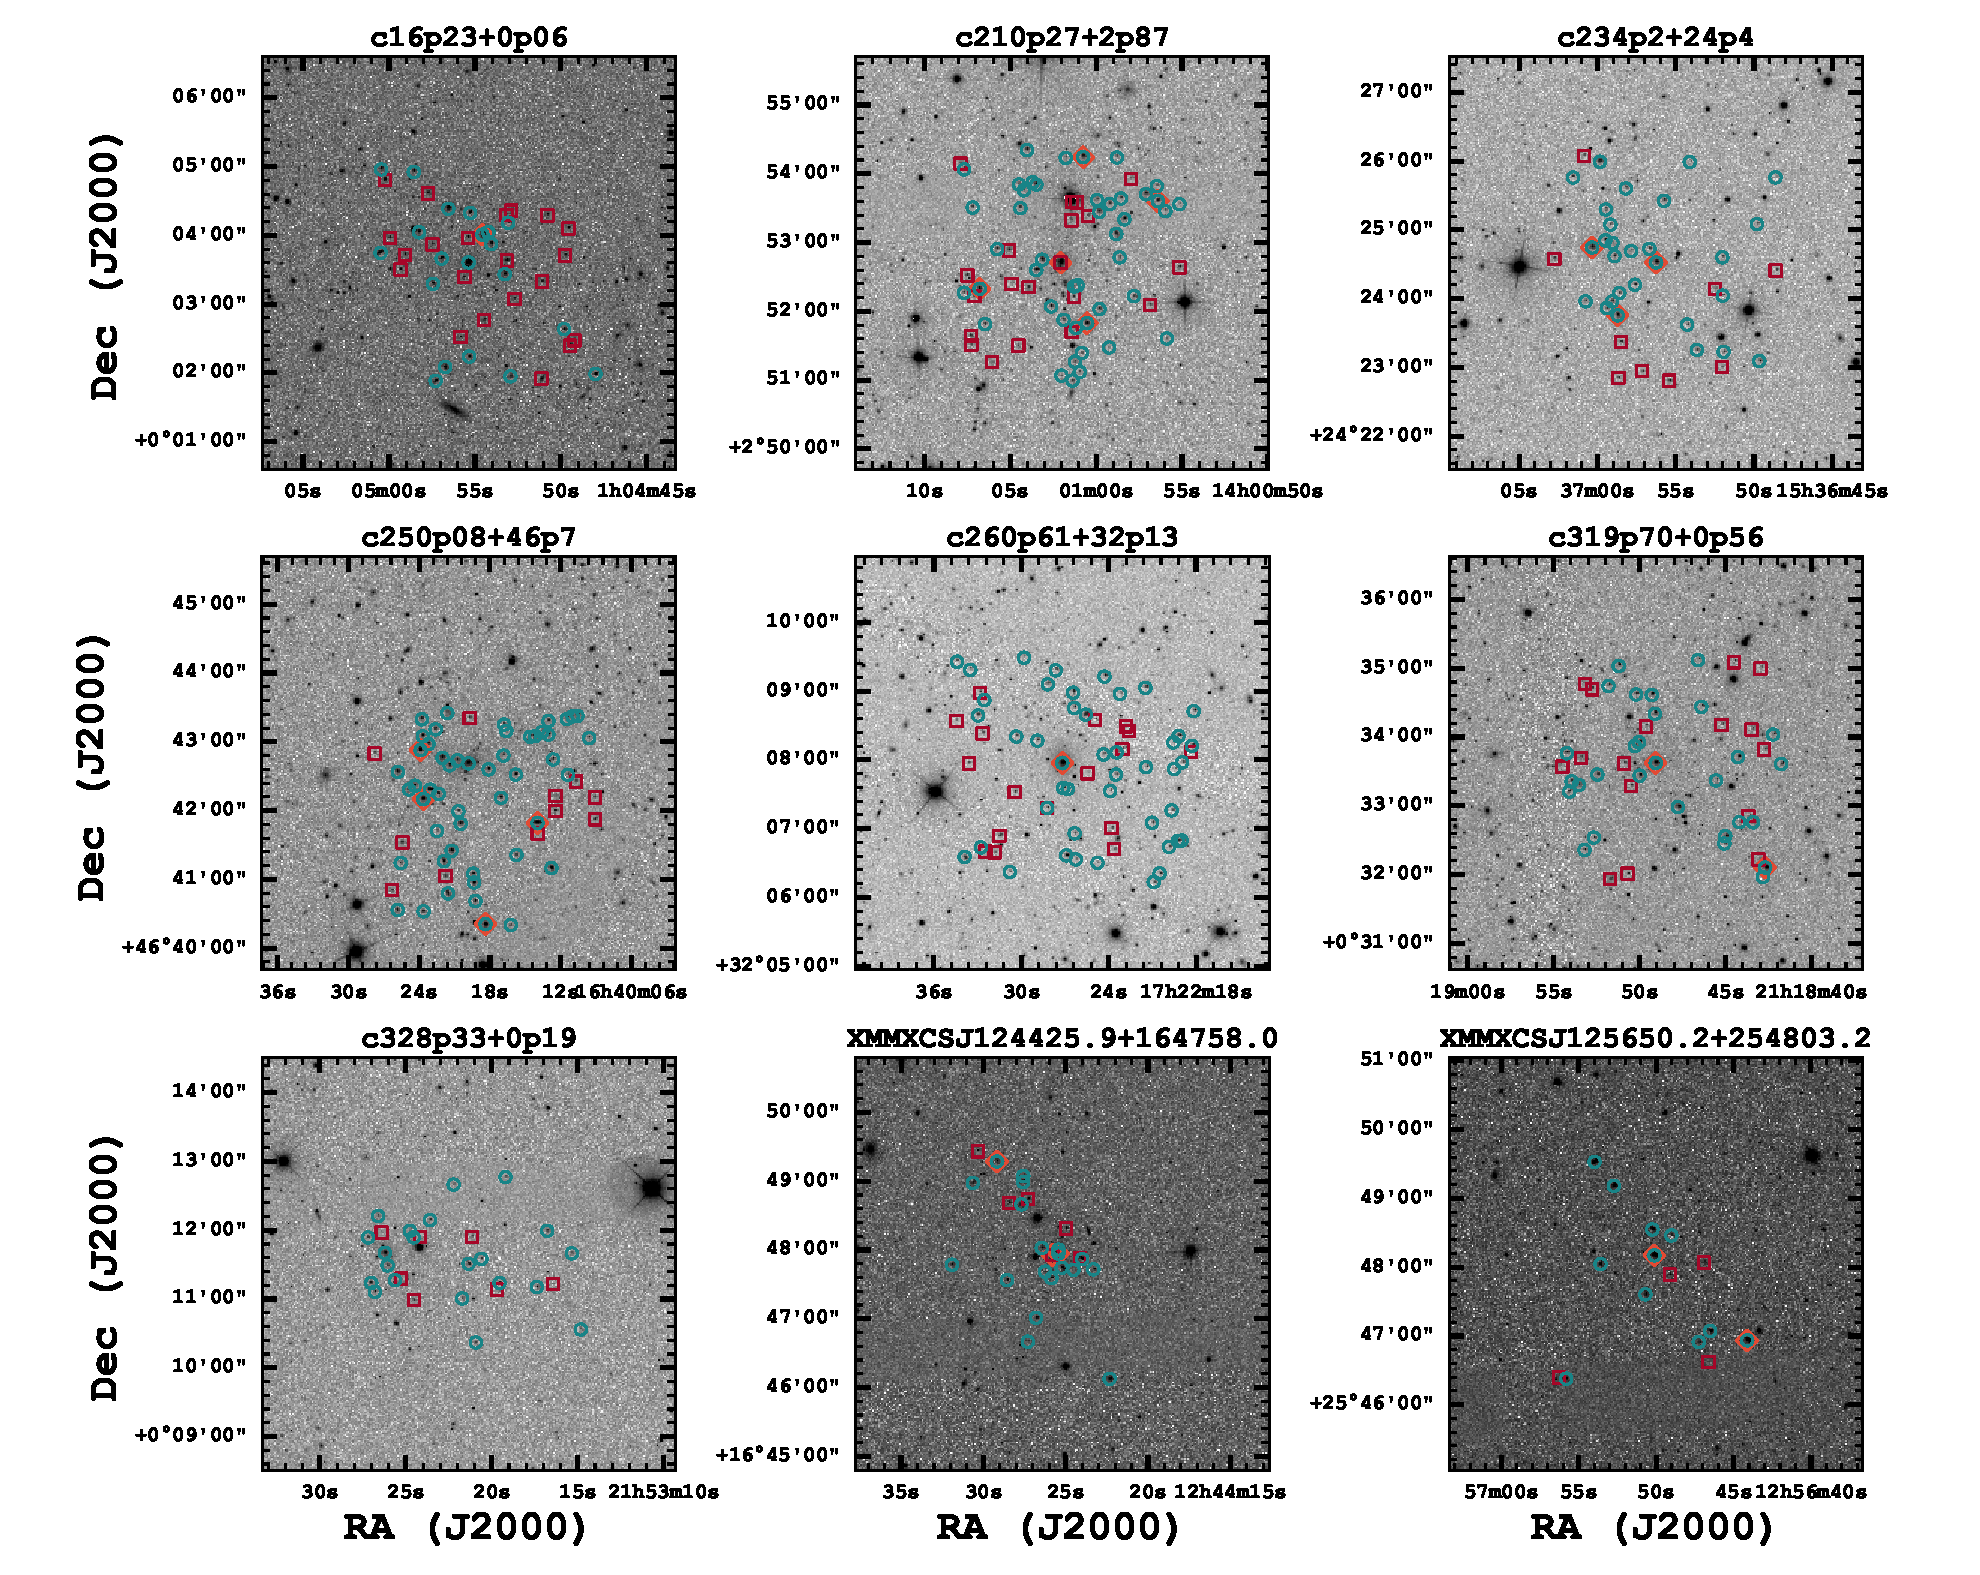
\includegraphics[width=\textwidth]{./figures2/multimontage.pdf}
\end{center}
	\caption[Montage of remaining nine clusters]{SDSS \sdssr\ image of cluster c203p83+41p0. The symbols show the position of observed galaxies. Blue circles indicate galaxies with $Q=0$ or $Q=1$ spectroscopic redshifts, red squares indicate galaxies where a redshift could not be reliably determined, and the orange diamond corresponds to galaxies with pre-existing redshifts from the SDSS. \textit{Right:} Example spectrum of an emission-line cluster galaxy (black line) and template fit (red line) from VIRUS-P on the McDonald 2.7m telescope. The spectrum shows the wavelength range and data quality expected from HETDEX-like spectroscopy, which are sufficient to measure galaxy redshifts.} 
	\label{2fig:montage}
\end{figure}


\begin{landscape}
	\begin{table}
		\centering 
		\caption[Spectroscopic redshifts for galaxies in MSJ010455.4+000336.3]{Spectroscopic redshifts for galaxies in MSJ010455.4+000336.3 measured with the MS: Columns as in Table~\ref{2tbl:MSJ133520.1+410004.1}.}
		\begin{tabular}{ccccccccccc}
			\hline
			tile & dither & fiber & ra & dec & r (mag) & redshift & Q & Member & R (Mpc) & LOSV (\kms) \\
			(1) & (2) & (3) & (4) & (5) & (6) & (7) & (8) & (9) & (10) & (11) \\
			\hline \hline
			NE & 1 & 223 & 01:04:56.937 & +00:03:39.60 & 19.38 & 0.2691$\pm{0.0002}$ & 0 & $\checkmark$ & 0.10 & -748$\pm{89}$ \\
			NE & 2 & 42 & 01:05:00.449 & +00:04:57.41 & 19.80 & 0.2766$\pm{0.0001}$ & 1 & $\checkmark$ & 0.47 & 1005$\pm{52}$ \\
			NE & 2 & 168 & 01:04:58.247 & +00:04:02.62 & 19.75 & 0.3054$\pm{0.0003}$ & 1 & ... & 0.23 & 7783$\pm{122}$ \\
			NE & 2 & 216 & 01:05:00.487 & +00:03:44.70 & 18.85 & 0.0826$\pm{0.0004}$ & 1 & ... & 0.12 & -44576$\pm{193}$ \\
			NE & 2 & 220 & 01:04:55.367 & +00:03:36.34 & 17.27 & 0.2715$\pm{0.0001}$ & 0 & $\checkmark$ & 0.00 & -193$\pm{61}$ \\
			NE & 3 & 38 & 01:04:58.559 & +00:04:55.13 & 19.95 & 0.3510$\pm{0.0001}$ & 1 & ... & 0.46 & 18494$\pm{56}$ \\
			NE & 3 & 106 & 01:04:56.545 & +00:04:23.15 & 18.36 & 0.2788$\pm{0.0001}$ & 0 & $\checkmark$ & 0.21 & 1517$\pm{47}$ \\
			NE & 3 & 118 & 01:04:55.276 & +00:04:19.53 & 19.49 & 0.2747$\pm{0.0001}$ & 0 & $\checkmark$ & 0.18 & 566$\pm{71}$ \\
			NE & 3 & 160 & 01:04:54.563 & +00:04:00.66 & 18.19 & 0.2747$\pm{0.0001}$ & 0 & $\checkmark$ & 0.11 & 559$\pm{52}$ \\
			NW & 1 & 156 & 01:04:53.064 & +00:04:10.99 & 20.22 & 0.2234$\pm{0.0001}$ & 1 & ... & 0.18 & -11495$\pm{52}$ \\
			NW & 2 & 173 & 01:04:54.217 & +00:04:02.78 & 19.62 & 0.2629$\pm{0.0002}$ & 0 & $\checkmark$ & 0.13 & -2205$\pm{80}$ \\
			NW & 3 & 187 & 01:04:54.051 & +00:03:52.42 & 19.35 & 0.3290$\pm{0.0001}$ & 1 & ... & 0.12 & 13319$\pm{52}$ \\
			SE & 1 & 50 & 01:04:57.440 & +00:03:17.71 & 19.51 & 0.2718$\pm{0.0002}$ & 1 & $\checkmark$ & 0.15 & -123$\pm{75}$ \\
			SE & 2 & 191 & 01:04:55.332 & +00:02:14.18 & 19.79 & 0.2794$\pm{0.0001}$ & 0 & $\checkmark$ & 0.35 & 1658$\pm{66}$ \\
			SE & 3 & 208 & 01:04:56.734 & +00:02:05.07 & 18.75 & 0.2781$\pm{0.0001}$ & 0 & $\checkmark$ & 0.40 & 1358$\pm{42}$ \\
			SE & 3 & 238 & 01:04:57.284 & +00:01:53.04 & 19.58 & 0.2705$\pm{0.0001}$ & 0 & $\checkmark$ & 0.45 & -421$\pm{66}$ \\
			SW & 2 & 26 & 01:04:53.268 & +00:03:26.04 & 18.99 & 0.2666$\pm{0.0002}$ & 0 & $\checkmark$ & 0.14 & -1352$\pm{85}$ \\
			SW & 2 & 135 & 01:04:49.814 & +00:02:38.18 & 20.10 & 0.2697$\pm{0.0002}$ & 1 & $\checkmark$ & 0.42 & -619$\pm{85}$ \\
			SW & 2 & 218 & 01:04:47.988 & +00:01:59.05 & 19.55 & 0.2627$\pm{0.0001}$ & 1 & $\checkmark$ & 0.60 & -2259$\pm{42}$ \\
			SW & 3 & 228 & 01:04:52.934 & +00:01:56.95 & 20.37 & 0.2763$\pm{0.0001}$ & 1 & $\checkmark$ & 0.45 & 928$\pm{47}$ \\
			\hline
		\end{tabular}
		\label{2tbl:MSJ010455.4+000336.3}
	\end{table}
\end{landscape}


\begin{landscape}
	\singlespace
	\begin{longtable}{ccccccccccc}
	\caption[Spectroscopic redshifts for galaxies in MSJ153656.3+242431.6]{Spectroscopic redshifts for galaxies in MSJ153656.3+242431.6 measured with the MS: Columns as in Table~\ref{2tbl:MSJ133520.1+410004.1}}\\
	\hline
	tile & dither & fiber & ra & dec & r (mag) & redshift & Q & Member & R (Mpc) & LOSV (\kms) \\
	(1) & (2) & (3) & (4) & (5) & (6) & (7) & (8) & (9) & (10) & (11) \\
	\hline \hline
	\endfirsthead
	\multicolumn{4}{l}%
	{\tablename\ \thetable\ Continued} \\
	\hline
	tile & dither & fiber & ra & dec & r (mag) & redshift & Q & Member & R (Mpc) & LOSV (\kms) \\
	(1) & (2) & (3) & (4) & (5) & (6) & (7) & (8) & (9) & (10) & (11) \\
	\hline \hline
	\endhead
	NE & 1 & 78 & 15:36:58.192 & +24:25:36.14 & 19.81 & 0.3228$\pm{0.0001}$ & 0 & ... & 0.33 & 23652$\pm{44}$ \\
	NE & 1 & 124 & 15:36:59.468 & +24:25:17.76 & 19.83 & 0.2324$\pm{0.0004}$ & 1 & $\checkmark$ & 0.24 & 1609$\pm{195}$ \\
	NE & 1 & 208 & 15:36:57.848 & +24:24:41.47 & 20.35 & 0.1881$\pm{0.0001}$ & 0 & ... & 0.08 & -9197$\pm{34}$ \\
	NE & 2 & 11 & 15:37:00.861 & +24:26:04.40 & 20.48 & 0.0947$\pm{0.0001}$ & 1 & ... & 0.20 & -31965$\pm{54}$ \\
	NE & 2 & 153 & 15:36:59.174 & +24:25:04.55 & 20.37 & 0.1036$\pm{0.0002}$ & 1 & ... & 0.10 & -29809$\pm{98}$ \\
	NE & 2 & 232 & 15:37:02.759 & +24:24:34.63 & 19.98 & 0.3017$\pm{0.0001}$ & 1 & ... & 0.40 & 18513$\pm{49}$ \\
	NE & 3 & 23 & 15:36:59.839 & +24:25:59.51 & 18.05 & 0.1275$\pm{0.0000}$ & 0 & ... & 0.23 & -23979$\pm{20}$ \\
	NE & 3 & 55 & 15:37:01.554 & +24:25:45.67 & 19.79 & 0.2115$\pm{0.0001}$ & 1 & ... & 0.36 & -3477$\pm{49}$ \\
	NE & 3 & 181 & 15:36:59.035 & +24:24:48.56 & 20.11 & 0.1874$\pm{0.0001}$ & 1 & ... & 0.13 & -9363$\pm{39}$ \\
	NE & 3 & 182 & 15:36:59.498 & +24:24:50.78 & 19.62 & 0.1231$\pm{0.0003}$ & 1 & ... & 0.11 & -25050$\pm{151}$ \\
	NE & 3 & 191 & 15:36:56.681 & +24:24:43.40 & 19.54 & 0.1808$\pm{0.0000}$ & 0 & ... & 0.04 & -10980$\pm{24}$ \\
	NE & 3 & 198 & 15:37:00.334 & +24:24:44.60 & 17.27 & 0.2274$\pm{0.0002}$ & 0 & $\checkmark$ & 0.21 & 387$\pm{112}$ \\
	NE & 3 & 210 & 15:36:58.911 & +24:24:37.07 & 19.67 & 0.4813$\pm{0.0000}$ & 1 & ... & 0.22 & 62324$\pm{24}$ \\
	NE & 3 & 219 & 15:36:56.253 & +24:24:31.59 & 17.36 & 0.2262$\pm{0.0001}$ & 0 & $\checkmark$ & 0.00 & 94$\pm{63}$ \\
	NW & 1 & 116 & 15:36:55.756 & +24:25:25.38 & 18.90 & 0.2706$\pm{0.0001}$ & 1 & ... & 0.23 & 10924$\pm{49}$ \\
	NW & 1 & 148 & 15:36:49.817 & +24:25:04.96 & 20.02 & 0.2224$\pm{0.0001}$ & 0 & $\checkmark$ & 0.34 & -813$\pm{63}$ \\
	NW & 2 & 26 & 15:36:54.106 & +24:25:59.10 & 20.79 & 0.2298$\pm{0.0000}$ & 0 & $\checkmark$ & 0.34 & 972$\pm{24}$ \\
	NW & 3 & 44 & 15:36:48.628 & +24:25:45.78 & 21.29 & 0.3341$\pm{0.0001}$ & 1 & ... & 0.62 & 26416$\pm{59}$ \\
	NW & 3 & 210 & 15:36:52.024 & +24:24:36.09 & 19.78 & 0.2281$\pm{0.0001}$ & 0 & $\checkmark$ & 0.21 & 570$\pm{63}$ \\
	SE & 1 & 48 & 15:36:57.612 & +24:24:12.18 & 19.43 & 0.2215$\pm{0.0002}$ & 0 & $\checkmark$ & 0.10 & -1038$\pm{78}$ \\
	SE & 1 & 64 & 15:36:58.605 & +24:24:04.80 & 20.06 & 0.2124$\pm{0.0001}$ & 1 & ... & 0.15 & -3277$\pm{59}$ \\
	SE & 2 & 80 & 15:36:59.058 & +24:23:57.63 & 19.24 & 0.2280$\pm{0.0002}$ & 0 & $\checkmark$ & 0.19 & 528$\pm{93}$ \\
	SE & 2 & 95 & 15:36:59.393 & +24:23:51.85 & 19.35 & 0.1244$\pm{0.0002}$ & 1 & ... & 0.13 & -24730$\pm{98}$ \\
	SE & 3 & 108 & 15:36:58.708 & +24:23:45.47 & 17.70 & 0.2235$\pm{0.0002}$ & 0 & $\checkmark$ & 0.21 & -565$\pm{83}$ \\
	SW & 1 & 66 & 15:36:52.487 & +24:24:08.35 & 20.29 & 0.1248$\pm{0.0001}$ & 1 & ... & 0.13 & -24633$\pm{63}$ \\
	SW & 1 & 142 & 15:36:54.270 & +24:23:37.37 & 20.15 & 0.2546$\pm{0.0001}$ & 0 & ... & 0.24 & 7019$\pm{54}$ \\
	SW & 2 & 185 & 15:36:53.657 & +24:23:15.33 & 19.58 & 0.2239$\pm{0.0002}$ & 0 & $\checkmark$ & 0.30 & -450$\pm{98}$ \\
	SW & 3 & 65 & 15:36:51.996 & +24:24:02.62 & 20.31 & 0.2201$\pm{0.0001}$ & 1 & $\checkmark$ & 0.23 & -1382$\pm{34}$ \\
	\hline
	\label{2tbl:MSJ153656.3+242431.6}
	\end{longtable}
\end{landscape}


\begin{landscape}
	\singlespace
	\begin{longtable}{ccccccccccc}
	\caption[Spectroscopic redshifts for galaxies in MSJ164019.8+464241.5]{Spectroscopic redshifts for galaxies in MSJ164019.8+464241.5 measured with the MS: Columns as in Table~\ref{2tbl:MSJ133520.1+410004.1}.}\\
	\hline
	tile & dither & fiber & ra & dec & r (mag) & redshift & Q & Member & R (Mpc) & LOSV (\kms) \\
	(1) & (2) & (3) & (4) & (5) & (6) & (7) & (8) & (9) & (10) & (11) \\
	\hline \hline
	\endfirsthead
	\multicolumn{4}{l}%
	{\tablename\ \thetable\ Continued} \\
	\hline
	tile & dither & fiber & ra & dec & r (mag) & redshift & Q & Member & R (Mpc) & LOSV (\kms) \\
	(1) & (2) & (3) & (4) & (5) & (6) & (7) & (8) & (9) & (10) & (11) \\
	\hline \hline
	\endhead
	NE & 1 & 34 & 16:40:21.617 & +46:43:25.07 & 20.12 & 0.1014$\pm{0.0003}$ & 0 & ... & 0.09 & -30528$\pm{141}$ \\
	NE & 1 & 110 & 16:40:23.879 & +46:42:52.76 & 17.81 & 0.2333$\pm{0.0000}$ & 0 & $\checkmark$ & 0.16 & 1617$\pm{24}$ \\
	NE & 1 & 133 & 16:40:19.812 & +46:42:41.30 & 16.61 & 0.2238$\pm{0.0001}$ & 0 & $\checkmark$ & 0.00 & -699$\pm{39}$ \\
	NE & 1 & 156 & 16:40:25.818 & +46:42:33.87 & 18.36 & 0.2099$\pm{0.0001}$ & 0 & ... & 0.21 & -4092$\pm{54}$ \\
	NE & 1 & 183 & 16:40:24.352 & +46:42:21.79 & 19.33 & 0.2248$\pm{0.0002}$ & 0 & $\checkmark$ & 0.18 & -462$\pm{93}$ \\
	NE & 1 & 211 & 16:40:23.651 & +46:42:10.01 & 17.62 & 0.2287$\pm{0.0001}$ & 0 & $\checkmark$ & 0.19 & 483$\pm{39}$ \\
	NE & 2 & 65 & 16:40:22.597 & +46:43:10.93 & 19.73 & 0.1813$\pm{0.0002}$ & 1 & ... & 0.13 & -11053$\pm{88}$ \\
	NE & 2 & 81 & 16:40:23.696 & +46:43:04.86 & 18.62 & 0.2324$\pm{0.0001}$ & 0 & $\checkmark$ & 0.17 & 1400$\pm{68}$ \\
	NE & 2 & 95 & 16:40:23.219 & +46:42:58.04 & 19.32 & 0.2264$\pm{0.0001}$ & 0 & $\checkmark$ & 0.14 & -75$\pm{39}$ \\
	NE & 2 & 122 & 16:40:22.018 & +46:42:46.03 & 18.84 & 0.2079$\pm{0.0001}$ & 0 & ... & 0.08 & -4574$\pm{73}$ \\
	NE & 2 & 136 & 16:40:21.428 & +46:42:39.59 & 19.11 & 0.2180$\pm{0.0002}$ & 0 & $\checkmark$ & 0.06 & -2120$\pm{93}$ \\
	NE & 2 & 195 & 16:40:22.346 & +46:42:14.63 & 19.21 & 0.2289$\pm{0.0002}$ & 0 & $\checkmark$ & 0.14 & 542$\pm{93}$ \\
	NE & 3 & 37 & 16:40:23.777 & +46:43:19.71 & 19.22 & 0.2229$\pm{0.0002}$ & 0 & $\checkmark$ & 0.20 & -933$\pm{102}$ \\
	NE & 3 & 120 & 16:40:20.755 & +46:42:43.96 & 17.82 & 0.2216$\pm{0.0002}$ & 0 & $\checkmark$ & 0.04 & -1240$\pm{83}$ \\
	NE & 3 & 181 & 16:40:23.067 & +46:42:18.32 & 18.39 & 0.2191$\pm{0.0001}$ & 0 & $\checkmark$ & 0.14 & -1852$\pm{39}$ \\
	NE & 3 & 184 & 16:40:24.861 & +46:42:18.39 & 19.09 & 0.2110$\pm{0.0002}$ & 0 & ... & 0.20 & -3816$\pm{78}$ \\
	NW & 1 & 50 & 16:40:13.038 & +46:43:18.14 & 19.37 & 0.2289$\pm{0.0002}$ & 0 & $\checkmark$ & 0.29 & 539$\pm{78}$ \\
	NW & 1 & 79 & 16:40:13.042 & +46:43:06.31 & 19.12 & 0.2297$\pm{0.0001}$ & 0 & $\checkmark$ & 0.27 & 730$\pm{34}$ \\
	NW & 1 & 81 & 16:40:14.572 & +46:43:04.50 & 20.49 & 0.2249$\pm{0.0002}$ & 1 & $\checkmark$ & 0.21 & -443$\pm{102}$ \\
	NW & 1 & 128 & 16:40:16.854 & +46:42:48.04 & 20.31 & 0.2281$\pm{0.0001}$ & 1 & $\checkmark$ & 0.11 & 342$\pm{68}$ \\
	NW & 1 & 215 & 16:40:17.060 & +46:42:11.27 & 19.21 & 0.2580$\pm{0.0002}$ & 1 & ... & 0.17 & 7632$\pm{122}$ \\
	NW & 2 & 33 & 16:40:10.991 & +46:43:22.18 & 19.33 & 0.2228$\pm{0.0001}$ & 1 & $\checkmark$ & 0.36 & -940$\pm{49}$ \\
	NW & 2 & 56 & 16:40:16.794 & +46:43:15.13 & 20.91 & 0.2350$\pm{0.0001}$ & 1 & $\checkmark$ & 0.17 & 2021$\pm{73}$ \\
	NW & 2 & 70 & 16:40:16.608 & +46:43:09.56 & 20.70 & 0.2167$\pm{0.0002}$ & 1 & $\checkmark$ & 0.15 & -2427$\pm{88}$ \\
	NW & 2 & 81 & 16:40:14.180 & +46:43:05.00 & 19.20 & 0.2252$\pm{0.0001}$ & 0 & $\checkmark$ & 0.23 & -375$\pm{68}$ \\
	NW & 2 & 156 & 16:40:15.807 & +46:42:31.47 & 18.88 & 0.2281$\pm{0.0002}$ & 0 & $\checkmark$ & 0.16 & 344$\pm{83}$ \\
	NW & 3 & 33 & 16:40:11.463 & +46:43:19.95 & 19.11 & 0.2249$\pm{0.0002}$ & 0 & $\checkmark$ & 0.34 & -426$\pm{97}$ \\
	NW & 3 & 65 & 16:40:13.553 & +46:43:08.81 & 20.49 & 0.1319$\pm{0.0001}$ & 1 & ... & 0.16 & -23097$\pm{29}$ \\
	NW & 3 & 74 & 16:40:09.583 & +46:43:03.29 & 20.34 & 0.1735$\pm{0.0001}$ & 1 & ... & 0.32 & -12967$\pm{58}$ \\
	NW & 3 & 122 & 16:40:12.635 & +46:42:44.68 & 19.66 & 0.2270$\pm{0.0001}$ & 0 & $\checkmark$ & 0.27 & 79$\pm{63}$ \\
	NW & 3 & 144 & 16:40:18.116 & +46:42:35.97 & 19.27 & 0.2080$\pm{0.0002}$ & 1 & ... & 0.06 & -4567$\pm{102}$ \\
	NW & 3 & 149 & 16:40:11.390 & +46:42:31.31 & 20.02 & 0.0844$\pm{0.0002}$ & 1 & ... & 0.14 & -34675$\pm{88}$ \\
	SE & 1 & 4 & 16:40:20.674 & +46:41:59.40 & 20.48 & 0.2341$\pm{0.0001}$ & 0 & $\checkmark$ & 0.16 & 1797$\pm{54}$ \\
	SE & 1 & 50 & 16:40:22.486 & +46:41:42.33 & 20.51 & 0.2376$\pm{0.0002}$ & 1 & ... & 0.25 & 2670$\pm{78}$ \\
	SE & 1 & 107 & 16:40:21.903 & +46:41:15.96 & 18.82 & 0.1866$\pm{0.0001}$ & 0 & ... & 0.28 & -9766$\pm{58}$ \\
	SE & 1 & 147 & 16:40:19.343 & +46:40:57.31 & 18.39 & 0.1864$\pm{0.0001}$ & 0 & ... & 0.33 & -9815$\pm{34}$ \\
	SE & 1 & 211 & 16:40:23.625 & +46:40:32.22 & 19.06 & 0.2325$\pm{0.0001}$ & 0 & $\checkmark$ & 0.50 & 1410$\pm{54}$ \\
	SE & 1 & 214 & 16:40:25.819 & +46:40:33.21 & 19.03 & 0.2272$\pm{0.0002}$ & 0 & $\checkmark$ & 0.52 & 113$\pm{93}$ \\
	SE & 2 & 113 & 16:40:25.565 & +46:41:14.28 & 20.51 & 0.2221$\pm{0.0002}$ & 0 & $\checkmark$ & 0.38 & -1116$\pm{83}$ \\
	SE & 2 & 165 & 16:40:21.553 & +46:40:47.83 & 18.59 & 0.2110$\pm{0.0001}$ & 1 & ... & 0.40 & -3819$\pm{68}$ \\
	SE & 3 & 18 & 16:40:20.484 & +46:41:48.57 & 18.80 & 0.2347$\pm{0.0001}$ & 0 & $\checkmark$ & 0.20 & 1960$\pm{58}$ \\
	SE & 3 & 77 & 16:40:21.250 & +46:41:25.01 & 18.21 & 0.1892$\pm{0.0001}$ & 0 & ... & 0.25 & -9128$\pm{29}$ \\
	SE & 3 & 118 & 16:40:19.417 & +46:41:05.03 & 19.40 & 0.2238$\pm{0.0002}$ & 0 & $\checkmark$ & 0.35 & -701$\pm{102}$ \\
	SE & 3 & 176 & 16:40:19.231 & +46:40:41.13 & 19.36 & 0.2167$\pm{0.0001}$ & 0 & ... & 0.42 & -2444$\pm{39}$ \\
	SW & 1 & 122 & 16:40:12.787 & +46:41:09.93 & 18.22 & 0.2340$\pm{0.0001}$ & 0 & $\checkmark$ & 0.44 & 1785$\pm{34}$ \\
	SW & 1 & 243 & 16:40:16.232 & +46:40:20.20 & 20.28 & 0.2278$\pm{0.0002}$ & 1 & $\checkmark$ & 0.53 & 274$\pm{88}$ \\
	SW & 1 & 246 & 16:40:18.377 & +46:40:20.93 & 17.51 & 0.1874$\pm{0.0002}$ & 0 & ... & 0.44 & -9576$\pm{107}$ \\
	SW & 2 & 98 & 16:40:15.754 & +46:41:21.37 & 20.03 & 0.2243$\pm{0.0001}$ & 0 & $\checkmark$ & 0.33 & -572$\pm{63}$ \\
	SW & 3 & 22 & 16:40:13.962 & +46:41:49.44 & 17.63 & 0.1107$\pm{0.0001}$ & 0 & ... & 0.16 & -28264$\pm{54}$ \\
	\hline
	\label{2tbl:MSJ164019.8+464241.5}
	\end{longtable}
\end{landscape}


\begin{landscape}
	\singlespace
	\begin{longtable}{ccccccccccc}
	\caption[Spectroscopic redshifts for galaxies in MSJ140102.0+025242.6]{Spectroscopic redshifts for galaxies in MSJ140102.0+025242.6 measured with the MS: Columns as in Table~\ref{2tbl:MSJ133520.1+410004.1}}\\
	\hline
	tile & dither & fiber & ra & dec & r (mag) & redshift & Q & Member & R (Mpc) & LOSV (\kms) \\
	(1) & (2) & (3) & (4) & (5) & (6) & (7) & (8) & (9) & (10) & (11) \\
	\hline \hline
	\endfirsthead
	\multicolumn{4}{l}%
	{\tablename\ \thetable\ Continued} \\
	\hline
	tile & dither & fiber & ra & dec & r (mag) & redshift & Q & Member & R (Mpc) & LOSV (\kms) \\
	(1) & (2) & (3) & (4) & (5) & (6) & (7) & (8) & (9) & (10) & (11) \\
	\hline \hline
	\endhead
	NE & 1 & 6 & 14:01:04.022 & +02:54:20.65 & 19.01 & 0.2478$\pm{0.0002}$ & 0 & $\checkmark$ & 0.40 & -1626$\pm{81}$ \\
	NE & 1 & 16 & 14:01:01.771 & +02:54:13.80 & 20.37 & 0.3158$\pm{0.0002}$ & 1 & ... & 0.42 & 14574$\pm{81}$ \\
	NE & 1 & 123 & 14:01:04.410 & +02:53:29.95 & 19.70 & 0.2325$\pm{0.0002}$ & 1 & ... & 0.22 & -5275$\pm{119}$ \\
	NE & 2 & 43 & 14:01:07.682 & +02:54:03.80 & 20.20 & 0.2039$\pm{0.0001}$ & 1 & ... & 0.40 & -12093$\pm{33}$ \\
	NE & 2 & 64 & 14:01:03.691 & +02:53:52.63 & 20.48 & 0.2876$\pm{0.0002}$ & 1 & ... & 0.32 & 7854$\pm{110}$ \\
	NE & 2 & 222 & 14:01:03.134 & +02:52:45.00 & 18.66 & 0.2517$\pm{0.0002}$ & 0 & $\checkmark$ & 0.07 & -699$\pm{91}$ \\
	NE & 3 & 63 & 14:01:03.475 & +02:53:50.51 & 18.68 & 0.2598$\pm{0.0002}$ & 0 & $\checkmark$ & 0.29 & 1217$\pm{110}$ \\
	NE & 3 & 65 & 14:01:04.494 & +02:53:50.70 & 20.31 & 0.2540$\pm{0.0002}$ & 0 & $\checkmark$ & 0.31 & -149$\pm{86}$ \\
	NE & 3 & 79 & 14:01:04.203 & +02:53:45.54 & 20.26 & 0.2192$\pm{0.0001}$ & 1 & ... & 0.25 & -8444$\pm{67}$ \\
	NE & 3 & 114 & 14:01:07.185 & +02:53:30.54 & 20.11 & 0.2606$\pm{0.0002}$ & 1 & $\checkmark$ & 0.37 & 1405$\pm{81}$ \\
	NE & 3 & 198 & 14:01:05.757 & +02:52:54.15 & 19.70 & 0.2516$\pm{0.0002}$ & 0 & $\checkmark$ & 0.23 & -737$\pm{114}$ \\
	NE & 3 & 237 & 14:01:03.483 & +02:52:35.96 & 18.94 & 0.3110$\pm{0.0001}$ & 1 & ... & 0.11 & 13416$\pm{52}$ \\
	NW & 1 & 23 & 14:00:58.786 & +02:54:14.18 & 20.07 & 0.2318$\pm{0.0001}$ & 1 & ... & 0.38 & -5458$\pm{71}$ \\
	NW & 1 & 92 & 14:00:57.098 & +02:53:42.10 & 18.42 & 0.2108$\pm{0.0002}$ & 0 & ... & 0.32 & -10444$\pm{119}$ \\
	NW & 1 & 105 & 14:00:56.404 & +02:53:36.25 & 18.55 & 0.2504$\pm{0.0002}$ & 0 & $\checkmark$ & 0.39 & -1030$\pm{91}$ \\
	NW & 1 & 111 & 14:00:59.191 & +02:53:33.62 & 19.78 & 0.2458$\pm{0.0002}$ & 0 & $\checkmark$ & 0.25 & -2108$\pm{105}$ \\
	NW & 2 & 103 & 14:00:55.146 & +02:53:33.41 & 21.44 & 0.1642$\pm{0.0003}$ & 1 & ... & 0.32 & -21563$\pm{143}$ \\
	NW & 2 & 119 & 14:00:55.968 & +02:53:27.36 & 20.34 & 0.3084$\pm{0.0003}$ & 1 & ... & 0.46 & 12808$\pm{129}$ \\
	NW & 2 & 127 & 14:00:59.815 & +02:53:26.69 & 19.29 & 0.2723$\pm{0.0001}$ & 1 & ... & 0.23 & 4205$\pm{38}$ \\
	NW & 3 & 13 & 14:01:00.752 & +02:54:14.53 & 17.96 & 0.2492$\pm{0.0002}$ & 1 & $\checkmark$ & 0.37 & -1312$\pm{81}$ \\
	NW & 3 & 62 & 14:00:56.466 & +02:53:49.12 & 20.53 & 0.3932$\pm{0.0001}$ & 1 & ... & 0.57 & 33012$\pm{67}$ \\
	NW & 3 & 95 & 14:00:58.558 & +02:53:38.37 & 20.03 & 0.2363$\pm{0.0001}$ & 1 & ... & 0.28 & -4369$\pm{48}$ \\
	NW & 3 & 98 & 14:00:59.942 & +02:53:37.00 & 20.63 & 0.4784$\pm{0.0000}$ & 1 & ... & 0.37 & 53304$\pm{24}$ \\
	NW & 3 & 138 & 14:00:58.352 & +02:53:20.29 & 18.69 & 0.2557$\pm{0.0002}$ & 0 & $\checkmark$ & 0.26 & 245$\pm{100}$ \\
	NW & 3 & 168 & 14:00:58.824 & +02:53:07.37 & 18.61 & 0.2321$\pm{0.0001}$ & 0 & ... & 0.20 & -5375$\pm{67}$ \\
	NW & 3 & 211 & 14:00:58.625 & +02:52:47.07 & 20.02 & 0.1463$\pm{0.0002}$ & 1 & ... & 0.13 & -25817$\pm{86}$ \\
	SE & 1 & 90 & 14:01:02.616 & +02:52:04.19 & 19.19 & 0.2639$\pm{0.0002}$ & 1 & $\checkmark$ & 0.16 & 2201$\pm{91}$ \\
	SE & 1 & 234 & 14:01:02.016 & +02:51:03.83 & 21.20 & 0.2830$\pm{0.0002}$ & 1 & ... & 0.42 & 6738$\pm{86}$ \\
	SE & 2 & 56 & 14:01:06.778 & +02:52:19.68 & 17.90 & 0.2249$\pm{0.0002}$ & 1 & ... & 0.27 & -7098$\pm{76}$ \\
	SE & 2 & 72 & 14:01:07.685 & +02:52:16.24 & 20.08 & 0.3193$\pm{0.0002}$ & 0 & ... & 0.42 & 15401$\pm{81}$ \\
	SE & 3 & 103 & 14:01:01.894 & +02:51:52.53 & 19.80 & 0.2437$\pm{0.0001}$ & 1 & $\checkmark$ & 0.19 & -2625$\pm{67}$ \\
	SE & 3 & 127 & 14:01:06.471 & +02:51:48.78 & 19.58 & 0.2726$\pm{0.0001}$ & 1 & ... & 0.36 & 4284$\pm{71}$ \\
	SW & 1 & 57 & 14:01:01.072 & +02:52:22.71 & 20.15 & 0.1615$\pm{0.0002}$ & 0 & ... & 0.07 & -22207$\pm{91}$ \\
	SW & 1 & 144 & 14:01:01.183 & +02:51:45.62 & 20.01 & 0.2670$\pm{0.0002}$ & 0 & $\checkmark$ & 0.24 & 2930$\pm{119}$ \\
	SW & 2 & 58 & 14:01:01.278 & +02:52:21.62 & 20.96 & 0.2581$\pm{0.0001}$ & 1 & $\checkmark$ & 0.09 & 821$\pm{57}$ \\
	SW & 2 & 65 & 14:00:57.802 & +02:52:13.21 & 20.18 & 0.4127$\pm{0.0002}$ & 1 & ... & 0.38 & 37664$\pm{86}$ \\
	SW & 2 & 98 & 14:00:59.802 & +02:52:01.88 & 19.31 & 0.2549$\pm{0.0002}$ & 1 & $\checkmark$ & 0.21 & 49$\pm{105}$ \\
	SW & 2 & 148 & 14:00:55.880 & +02:51:36.29 & 21.24 & 0.1548$\pm{0.0002}$ & 1 & ... & 0.30 & -23794$\pm{119}$ \\
	SW & 2 & 231 & 14:01:00.954 & +02:51:06.98 & 20.55 & 0.3329$\pm{0.0001}$ & 1 & ... & 0.46 & 18635$\pm{62}$ \\
	SW & 3 & 128 & 14:01:00.529 & +02:51:49.71 & 18.25 & 0.2628$\pm{0.0003}$ & 1 & $\checkmark$ & 0.23 & 1934$\pm{153}$ \\
	SW & 3 & 169 & 14:00:59.240 & +02:51:28.42 & 21.07 & 0.4035$\pm{0.0001}$ & 1 & ... & 0.46 & 35457$\pm{57}$ \\
	SW & 3 & 187 & 14:01:00.832 & +02:51:23.59 & 20.68 & 0.1628$\pm{0.0001}$ & 1 & ... & 0.23 & -21887$\pm{52}$ \\
	SW & 3 & 202 & 14:01:01.230 & +02:51:16.08 & 19.95 & 0.2355$\pm{0.0002}$ & 0 & ... & 0.33 & -4560$\pm{76}$ \\
	SW & 3 & 246 & 14:01:01.370 & +02:50:59.59 & 20.01 & 0.2207$\pm{0.0001}$ & 1 & ... & 0.37 & -8106$\pm{62}$ \\
			\hline
	\label{2tbl:MSJ140102.0+025242.6}
	\end{longtable}
\end{landscape}


\begin{landscape}
	\singlespace
	\begin{longtable}{ccccccccccc}
	\caption[Spectroscopic redshifts for galaxies in MSJ172227.2+320757.2]{Spectroscopic redshifts for galaxies in MSJ172227.2+320757.2 measured with the MS: Columns as in Table~\ref{2tbl:MSJ133520.1+410004.1}}\\
	\hline
	tile & dither & fiber & ra & dec & r (mag) & redshift & Q & Member & R (Mpc) & LOSV (\kms) \\
	(1) & (2) & (3) & (4) & (5) & (6) & (7) & (8) & (9) & (10) & (11) \\
	\hline \hline
	\endfirsthead
	\multicolumn{4}{l}%
	{\tablename\ \thetable\ Continued} \\
	\hline
	tile & dither & fiber & ra & dec & r (mag) & redshift & Q & Member & R (Mpc) & LOSV (\kms) \\
	(1) & (2) & (3) & (4) & (5) & (6) & (7) & (8) & (9) & (10) & (11) \\
	\hline \hline
	\endhead
	NE & 1 & 21 & 17:22:29.818 & +32:09:29.21 & 20.20 & 0.1014$\pm{0.0004}$ & 0 & ... & 0.18 & -30318$\pm{200}$ \\
	NE & 1 & 29 & 17:22:34.413 & +32:09:25.72 & 19.68 & 0.2321$\pm{0.0001}$ & 0 & $\checkmark$ & 0.47 & 1553$\pm{34}$ \\
	NE & 2 & 32 & 17:22:27.631 & +32:09:18.17 & 19.76 & 0.2200$\pm{0.0002}$ & 0 & ... & 0.29 & -1396$\pm{78}$ \\
	NE & 2 & 62 & 17:22:28.177 & +32:09:05.94 & 19.38 & 0.2246$\pm{0.0001}$ & 1 & $\checkmark$ & 0.25 & -282$\pm{34}$ \\
	NE & 2 & 179 & 17:22:28.895 & +32:08:16.78 & 19.86 & 0.2332$\pm{0.0002}$ & 1 & $\checkmark$ & 0.11 & 1819$\pm{93}$ \\
	NE & 3 & 42 & 17:22:33.506 & +32:09:18.50 & 20.35 & 0.2318$\pm{0.0001}$ & 1 & $\checkmark$ & 0.42 & 1492$\pm{44}$ \\
	NE & 3 & 73 & 17:22:26.441 & +32:08:58.70 & 19.12 & 0.2084$\pm{0.0001}$ & 0 & ... & 0.21 & -4221$\pm{34}$ \\
	NE & 3 & 98 & 17:22:32.542 & +32:08:52.14 & 20.50 & 0.2100$\pm{0.0003}$ & 1 & ... & 0.30 & -3831$\pm{161}$ \\
	NE & 3 & 102 & 17:22:26.378 & +32:08:45.31 & 19.76 & 0.1683$\pm{0.0001}$ & 0 & ... & 0.14 & -14010$\pm{44}$ \\
	NE & 3 & 128 & 17:22:32.971 & +32:08:38.74 & 19.34 & 0.2315$\pm{0.0001}$ & 1 & ... & 0.31 & 1419$\pm{44}$ \\
	NE & 3 & 167 & 17:22:30.347 & +32:08:20.40 & 19.86 & 0.2909$\pm{0.0002}$ & 1 & ... & 0.20 & 15894$\pm{117}$ \\
	NE & 3 & 219 & 17:22:27.184 & +32:07:57.25 & 15.38 & 0.2226$\pm{0.0002}$ & 0 & $\checkmark$ & 0.00 & -762$\pm{78}$ \\
	NW & 1 & 102 & 17:22:18.160 & +32:08:42.50 & 18.84 & 0.2228$\pm{0.0001}$ & 0 & $\checkmark$ & 0.44 & -716$\pm{63}$ \\
	NW & 1 & 200 & 17:22:24.352 & +32:08:04.74 & 20.42 & 0.2744$\pm{0.0001}$ & 1 & ... & 0.15 & 11881$\pm{44}$ \\
	NW & 1 & 205 & 17:22:18.953 & +32:07:57.82 & 19.67 & 0.2275$\pm{0.0001}$ & 0 & $\checkmark$ & 0.38 & 433$\pm{44}$ \\
	NW & 2 & 68 & 17:22:23.220 & +32:08:57.64 & 21.00 & 0.2798$\pm{0.0002}$ & 1 & ... & 0.33 & 13189$\pm{88}$ \\
	NW & 2 & 116 & 17:22:25.574 & +32:08:39.54 & 17.80 & 0.1685$\pm{0.0001}$ & 0 & ... & 0.14 & -13964$\pm{54}$ \\
	NW & 2 & 148 & 17:22:19.197 & +32:08:20.80 & 18.98 & 0.2245$\pm{0.0001}$ & 0 & $\checkmark$ & 0.38 & -304$\pm{44}$ \\
	NW & 2 & 161 & 17:22:18.289 & +32:08:12.33 & 19.59 & 0.2203$\pm{0.0002}$ & 0 & $\checkmark$ & 0.41 & -1318$\pm{98}$ \\
	NW & 2 & 163 & 17:22:19.559 & +32:08:15.27 & 19.47 & 0.2143$\pm{0.0001}$ & 0 & ... & 0.34 & -2782$\pm{63}$ \\
	NW & 3 & 26 & 17:22:24.290 & +32:09:12.65 & 19.16 & 0.1680$\pm{0.0003}$ & 0 & ... & 0.24 & -14079$\pm{137}$ \\
	NW & 3 & 50 & 17:22:21.475 & +32:09:02.84 & 19.02 & 0.2260$\pm{0.0002}$ & 0 & $\checkmark$ & 0.36 & 55$\pm{98}$ \\
	NW & 3 & 184 & 17:22:23.454 & +32:08:06.50 & 19.96 & 0.2628$\pm{0.0001}$ & 1 & ... & 0.20 & 9047$\pm{68}$ \\
	NW & 3 & 206 & 17:22:19.500 & +32:07:52.06 & 20.94 & 0.2185$\pm{0.0001}$ & 1 & $\checkmark$ & 0.35 & -1753$\pm{39}$ \\
	SE & 1 & 202 & 17:22:33.893 & +32:06:35.34 & 18.68 & 0.2203$\pm{0.0001}$ & 1 & $\checkmark$ & 0.42 & -1333$\pm{59}$ \\
	SE & 2 & 91 & 17:22:28.227 & +32:07:18.12 & 20.29 & 0.2135$\pm{0.0001}$ & 0 & ... & 0.14 & -2982$\pm{63}$ \\
	SE & 2 & 189 & 17:22:26.261 & +32:06:33.18 & 20.64 & 0.2897$\pm{0.0002}$ & 1 & ... & 0.37 & 15599$\pm{122}$ \\
	SE & 2 & 226 & 17:22:30.791 & +32:06:22.27 & 20.60 & 0.2482$\pm{0.0001}$ & 1 & ... & 0.41 & 5478$\pm{39}$ \\
	SE & 3 & 45 & 17:22:27.117 & +32:07:35.51 & 19.77 & 0.2210$\pm{0.0003}$ & 0 & $\checkmark$ & 0.08 & -1157$\pm{151}$ \\
	SE & 3 & 171 & 17:22:32.779 & +32:06:43.69 & 20.61 & 0.2261$\pm{0.0000}$ & 0 & $\checkmark$ & 0.37 & 92$\pm{24}$ \\
	SW & 1 & 160 & 17:22:18.982 & +32:06:49.70 & 19.60 & 0.2262$\pm{0.0001}$ & 0 & $\checkmark$ & 0.45 & 121$\pm{44}$ \\
	SW & 1 & 203 & 17:22:26.919 & +32:06:36.74 & 18.29 & 0.2256$\pm{0.0002}$ & 0 & $\checkmark$ & 0.29 & -30$\pm{78}$ \\
	SW & 1 & 214 & 17:22:24.770 & +32:06:30.20 & 20.93 & 0.2334$\pm{0.0001}$ & 1 & $\checkmark$ & 0.34 & 1880$\pm{68}$ \\
	SW & 2 & 121 & 17:22:21.021 & +32:07:05.24 & 19.59 & 0.2293$\pm{0.0002}$ & 0 & $\checkmark$ & 0.35 & 882$\pm{78}$ \\
	SW & 3 & 5 & 17:22:21.443 & +32:07:53.68 & 19.98 & 0.1781$\pm{0.0002}$ & 0 & ... & 0.22 & -11617$\pm{117}$ \\
	SW & 3 & 23 & 17:22:23.499 & +32:07:47.19 & 19.62 & 0.1771$\pm{0.0001}$ & 0 & ... & 0.14 & -11852$\pm{29}$ \\
	SW & 3 & 53 & 17:22:23.894 & +32:07:32.82 & 20.45 & 0.3593$\pm{0.0001}$ & 1 & ... & 0.24 & 32587$\pm{29}$ \\
	SW & 3 & 58 & 17:22:26.813 & +32:07:34.55 & 19.46 & 0.2238$\pm{0.0001}$ & 0 & $\checkmark$ & 0.08 & -474$\pm{68}$ \\
	SW & 3 & 89 & 17:22:19.677 & +32:07:15.96 & 19.83 & 0.2258$\pm{0.0001}$ & 0 & $\checkmark$ & 0.38 & 21$\pm{63}$ \\
	SW & 3 & 144 & 17:22:26.332 & +32:06:55.93 & 20.24 & 0.2292$\pm{0.0001}$ & 1 & $\checkmark$ & 0.23 & 845$\pm{73}$ \\
	SW & 3 & 146 & 17:22:19.254 & +32:06:49.42 & 19.04 & 0.2258$\pm{0.0001}$ & 0 & $\checkmark$ & 0.44 & 18$\pm{59}$ \\
	SW & 3 & 162 & 17:22:19.860 & +32:06:44.09 & 19.95 & 0.3840$\pm{0.0001}$ & 1 & ... & 0.62 & 38622$\pm{73}$ \\
	SW & 3 & 221 & 17:22:20.506 & +32:06:21.01 & 19.35 & 0.2242$\pm{0.0002}$ & 0 & $\checkmark$ & 0.46 & -372$\pm{78}$ \\
	SW & 3 & 236 & 17:22:20.911 & +32:06:13.52 & 20.04 & 0.1851$\pm{0.0001}$ & 1 & ... & 0.41 & -9900$\pm{39}$ \\
	\hline
	\label{2tbl:MSJ172227.2+320757.2}
	\end{longtable}
\end{landscape}


\begin{landscape}
	\singlespace
	\begin{longtable}{ccccccccccc}
	\caption[Spectroscopic redshifts for galaxies in MSJ211849.1+003337.3]{Spectroscopic redshifts for galaxies in MSJ211849.1+003337.3 measured with the MS: Columns as in Table~\ref{2tbl:MSJ133520.1+410004.1}}\\
	\hline
	tile & dither & fiber & ra & dec & r (mag) & redshift & Q & Member & R (Mpc) & LOSV (\kms) \\
	(1) & (2) & (3) & (4) & (5) & (6) & (7) & (8) & (9) & (10) & (11) \\
	\hline \hline
	\endfirsthead
	\multicolumn{4}{l}%
	{\tablename\ \thetable\ Continued} \\
	\hline
	tile & dither & fiber & ra & dec & r (mag) & redshift & Q & Member & R (Mpc) & LOSV (\kms) \\
	(1) & (2) & (3) & (4) & (5) & (6) & (7) & (8) & (9) & (10) & (11) \\
	\hline \hline
	\endhead
	NE & 1 & 193 & 21:18:50.285 & +00:33:52.08 & 20.09 & 0.2785$\pm{0.0002}$ & 0 & $\checkmark$ & 0.10 & 633$\pm{112}$ \\
	NE & 1 & 216 & 21:18:54.243 & +00:33:45.76 & 19.71 & 0.2765$\pm{0.0001}$ & 0 & $\checkmark$ & 0.33 & 169$\pm{66}$ \\
	NE & 2 & 220 & 21:18:49.071 & +00:33:37.32 & 17.42 & 0.2756$\pm{0.0001}$ & 0 & $\checkmark$ & 0.00 & -37$\pm{47}$ \\
	NE & 3 & 21 & 21:18:51.226 & +00:35:01.96 & 19.56 & 0.2740$\pm{0.0002}$ & 1 & $\checkmark$ & 0.38 & -424$\pm{103}$ \\
	NE & 3 & 66 & 21:18:51.814 & +00:34:44.38 & 20.20 & 0.3058$\pm{0.0004}$ & 1 & ... & 0.36 & 7022$\pm{169}$ \\
	NE & 3 & 75 & 21:18:49.304 & +00:34:36.62 & 19.15 & 0.1346$\pm{0.0001}$ & 0 & ... & 0.14 & -33096$\pm{66}$ \\
	NE & 3 & 77 & 21:18:50.210 & +00:34:37.07 & 20.14 & 0.2195$\pm{0.0003}$ & 1 & ... & 0.22 & -13192$\pm{127}$ \\
	NE & 3 & 118 & 21:18:49.121 & +00:34:20.26 & 18.85 & 0.2610$\pm{0.0003}$ & 1 & ... & 0.17 & -3470$\pm{127}$ \\
	NE & 3 & 178 & 21:18:50.051 & +00:33:55.37 & 19.01 & 0.3132$\pm{0.0004}$ & 1 & ... & 0.11 & 8768$\pm{192}$ \\
	NW & 1 & 25 & 21:18:46.617 & +00:35:06.97 & 20.60 & 0.2727$\pm{0.0001}$ & 0 & $\checkmark$ & 0.41 & -724$\pm{70}$ \\
	NW & 2 & 112 & 21:18:46.414 & +00:34:26.28 & 20.33 & 0.2621$\pm{0.0001}$ & 0 & ... & 0.26 & -3217$\pm{70}$ \\
	NW & 2 & 209 & 21:18:44.289 & +00:33:42.58 & 19.24 & 0.2688$\pm{0.0001}$ & 0 & $\checkmark$ & 0.30 & -1645$\pm{61}$ \\
	NW & 3 & 161 & 21:18:42.244 & +00:34:02.14 & 20.31 & 0.2735$\pm{0.0002}$ & 0 & $\checkmark$ & 0.44 & -531$\pm{84}$ \\
	NW & 3 & 218 & 21:18:41.776 & +00:33:36.44 & 19.08 & 0.1644$\pm{0.0001}$ & 0 & ... & 0.31 & -26114$\pm{66}$ \\
	SE & 1 & 55 & 21:18:53.543 & +00:33:18.15 & 18.90 & 0.2717$\pm{0.0001}$ & 0 & $\checkmark$ & 0.29 & -953$\pm{61}$ \\
	SE & 1 & 185 & 21:18:53.214 & +00:32:21.39 & 20.36 & 0.2774$\pm{0.0002}$ & 1 & $\checkmark$ & 0.42 & 369$\pm{80}$ \\
	SE & 2 & 19 & 21:18:50.005 & +00:33:26.22 & 19.07 & 0.2794$\pm{0.0002}$ & 0 & $\checkmark$ & 0.08 & 842$\pm{80}$ \\
	SE & 2 & 24 & 21:18:52.466 & +00:33:27.23 & 19.30 & 0.2786$\pm{0.0001}$ & 0 & $\checkmark$ & 0.22 & 652$\pm{61}$ \\
	SE & 2 & 42 & 21:18:53.957 & +00:33:21.27 & 19.97 & 0.2754$\pm{0.0001}$ & 0 & $\checkmark$ & 0.32 & -105$\pm{61}$ \\
	SE & 2 & 155 & 21:18:52.670 & +00:32:32.22 & 20.33 & 0.2132$\pm{0.0003}$ & 1 & ... & 0.29 & -14680$\pm{131}$ \\
	SE & 3 & 56 & 21:18:54.097 & +00:33:12.36 & 19.86 & 0.2284$\pm{0.0000}$ & 0 & ... & 0.29 & -11096$\pm{9}$ \\
	SW & 1 & 100 & 21:18:47.781 & +00:32:58.96 & 18.20 & 0.2276$\pm{0.0000}$ & 0 & ... & 0.16 & -11305$\pm{23}$ \\
	SW & 1 & 120 & 21:18:43.405 & +00:32:45.55 & 19.22 & 0.2811$\pm{0.0002}$ & 0 & $\checkmark$ & 0.42 & 1236$\pm{89}$ \\
	SW & 1 & 152 & 21:18:45.023 & +00:32:33.46 & 18.62 & 0.2770$\pm{0.0001}$ & 0 & $\checkmark$ & 0.37 & 291$\pm{42}$ \\
	SW & 1 & 167 & 21:18:45.081 & +00:32:27.08 & 19.91 & 0.2786$\pm{0.0002}$ & 0 & $\checkmark$ & 0.39 & 669$\pm{80}$ \\
	SW & 2 & 38 & 21:18:45.564 & +00:33:22.07 & 20.54 & 0.3010$\pm{0.0001}$ & 1 & ... & 0.24 & 5907$\pm{28}$ \\
	SW & 2 & 122 & 21:18:44.203 & +00:32:45.66 & 20.29 & 0.2775$\pm{0.0001}$ & 0 & $\checkmark$ & 0.38 & 404$\pm{66}$ \\
	SW & 2 & 206 & 21:18:42.699 & +00:32:06.10 & 17.62 & 0.2700$\pm{0.0001}$ & 0 & $\checkmark$ & 0.55 & -1356$\pm{33}$ \\
	SW & 3 & 220 & 21:18:42.834 & +00:31:57.86 & 21.05 & 0.2739$\pm{0.0000}$ & 0 & $\checkmark$ & 0.57 & -440$\pm{19}$ \\
			\hline
		\label{2tbl:MSJ211849.1+003337.3}
	\end{longtable}
\end{landscape}


\begin{landscape}
	\begin{table}
		\centering 
		\caption[Spectroscopic redshifts for galaxies in MSJ215422.9+003723.5]{Spectroscopic redshifts for galaxies in MSJ215422.9+003723.5 measured with the MS: Columns as in Table~\ref{2tbl:MSJ133520.1+410004.1}}
		\begin{tabular}{ccccccccccc}
			\hline
			tile & dither & fiber & ra & dec & r (mag) & redshift & Q & Member & R (Mpc) & LOSV (\kms) \\
			(1) & (2) & (3) & (4) & (5) & (6) & (7) & (8) & (9) & (10) & (11) \\
			\hline \hline
	NE & 1 & 62 & 21:53:22.219 & +00:12:39.81 & 20.97 & 0.0766$\pm{0.0001}$ & 1 & ... & 0.10 & -34369$\pm{34}$ \\
	NE & 1 & 215 & 21:53:26.220 & +00:11:40.21 & 16.71 & 0.2159$\pm{0.0001}$ & 0 & $\checkmark$ & 0.26 & -146$\pm{44}$ \\
	NE & 2 & 138 & 21:53:23.595 & +00:12:08.78 & 20.12 & 0.2737$\pm{0.0002}$ & 0 & ... & 0.21 & 14070$\pm{88}$ \\
	NE & 2 & 220 & 21:53:21.347 & +00:11:30.70 & 19.12 & 0.2192$\pm{0.0002}$ & 0 & $\checkmark$ & 0.00 & 667$\pm{79}$ \\
	NE & 3 & 129 & 21:53:26.616 & +00:12:12.42 & 19.97 & 0.2172$\pm{0.0002}$ & 0 & $\checkmark$ & 0.32 & 178$\pm{84}$ \\
	NE & 3 & 154 & 21:53:24.770 & +00:11:59.52 & 20.86 & 0.2809$\pm{0.0000}$ & 0 & ... & 0.25 & 15838$\pm{25}$ \\
	NE & 3 & 168 & 21:53:24.545 & +00:11:53.74 & 21.00 & 0.2210$\pm{0.0001}$ & 0 & $\checkmark$ & 0.19 & 1119$\pm{44}$ \\
	NE & 3 & 174 & 21:53:27.197 & +00:11:53.68 & 19.85 & 0.2161$\pm{0.0001}$ & 0 & $\checkmark$ & 0.32 & -92$\pm{69}$ \\
	NW & 1 & 206 & 21:53:15.345 & +00:11:39.78 & 19.96 & 0.2170$\pm{0.0001}$ & 0 & $\checkmark$ & 0.32 & 131$\pm{44}$ \\
	NW & 2 & 55 & 21:53:19.205 & +00:12:46.30 & 20.20 & 0.2134$\pm{0.0002}$ & 0 & $\checkmark$ & 0.29 & -751$\pm{108}$ \\
	NW & 3 & 151 & 21:53:16.776 & +00:11:59.52 & 19.20 & 0.2166$\pm{0.0001}$ & 0 & $\checkmark$ & 0.26 & 45$\pm{39}$ \\
	NW & 3 & 217 & 21:53:20.606 & +00:11:34.95 & 20.71 & 0.2188$\pm{0.0002}$ & 1 & $\checkmark$ & 0.04 & 586$\pm{98}$ \\
	SE & 1 & 12 & 21:53:26.058 & +00:11:29.27 & 19.79 & 0.2164$\pm{0.0001}$ & 0 & $\checkmark$ & 0.25 & -19$\pm{59}$ \\
	SE & 1 & 40 & 21:53:25.627 & +00:11:16.34 & 18.96 & 0.2164$\pm{0.0001}$ & 0 & $\checkmark$ & 0.23 & -9$\pm{49}$ \\
	SE & 3 & 43 & 21:53:27.012 & +00:11:14.01 & 19.55 & 0.2159$\pm{0.0002}$ & 0 & $\checkmark$ & 0.30 & -127$\pm{88}$ \\
	SE & 3 & 57 & 21:53:26.805 & +00:11:06.27 & 19.54 & 0.2143$\pm{0.0001}$ & 0 & $\checkmark$ & 0.30 & -537$\pm{54}$ \\
	SE & 3 & 61 & 21:53:21.720 & +00:11:00.41 & 20.37 & 0.2144$\pm{0.0001}$ & 0 & $\checkmark$ & 0.11 & -510$\pm{59}$ \\
	SW & 1 & 51 & 21:53:17.384 & +00:11:10.44 & 19.13 & 0.2189$\pm{0.0001}$ & 0 & $\checkmark$ & 0.22 & 608$\pm{34}$ \\
	SW & 1 & 174 & 21:53:20.933 & +00:10:22.05 & 19.86 & 0.3719$\pm{0.0001}$ & 0 & ... & 0.36 & 38208$\pm{34}$ \\
	SW & 2 & 133 & 21:53:14.825 & +00:10:33.36 & 20.80 & 0.2085$\pm{0.0002}$ & 0 & ... & 0.39 & -1958$\pm{84}$ \\
	SW & 3 & 41 & 21:53:19.548 & +00:11:13.96 & 19.84 & 0.2138$\pm{0.0001}$ & 0 & $\checkmark$ & 0.11 & -658$\pm{39}$ \\
			\hline
		\end{tabular}
		\label{2tbl:MSJ215422.9+003723.5}
	\end{table}
\end{landscape}


\begin{landscape}
	\begin{table}
		\centering 
		\caption[Spectroscopic redshifts for galaxies in XMMXCSJ124425.9+164758.0.]{Spectroscopic redshifts for galaxies in XMMXCSJ124425.9+164758.0: Columns as in Table~\ref{2tbl:MSJ133520.1+410004.1}}
		\begin{tabular}{ccccccccccc}
			\hline
			tile & dither & fiber & ra & dec & r (mag) & redshift & Q & Member & R (Mpc) & LOSV (\kms) \\
			(1) & (2) & (3) & (4) & (5) & (6) & (7) & (8) & (9) & (10) & (11) \\
			\hline \hline
	NE & 1 & 39 & 12:44:29.179 & +16:49:17.17 & 19.38 & 0.4514$\pm{0.0001}$ & 0 & ... & 0.61 & 53398$\pm{44}$ \\
	NE & 1 & 79 & 12:44:27.588 & +16:48:59.30 & 20.00 & 0.2235$\pm{0.0001}$ & 1 & ... & 0.29 & -1943$\pm{44}$ \\
	NE & 1 & 85 & 12:44:30.641 & +16:48:58.51 & 19.65 & 0.2376$\pm{0.0001}$ & 0 & ... & 0.40 & 1475$\pm{39}$ \\
	NE & 1 & 207 & 12:44:26.458 & +16:48:01.70 & 20.04 & 0.2372$\pm{0.0002}$ & 1 & ... & 0.09 & 1398$\pm{92}$ \\
	NE & 2 & 65 & 12:44:27.576 & +16:49:04.52 & 20.86 & 0.2529$\pm{0.0001}$ & 1 & ... & 0.33 & 5207$\pm{39}$ \\
	NE & 2 & 123 & 12:44:27.689 & +16:48:39.78 & 18.94 & 0.1079$\pm{0.0001}$ & 1 & ... & 0.12 & -29994$\pm{63}$ \\
	NE & 3 & 205 & 12:44:25.438 & +16:48:00.39 & 18.15 & 0.2313$\pm{0.0002}$ & 0 & $\checkmark$ & 0.05 & -52$\pm{78}$ \\
	NW & 1 & 17 & 12:44:23.999 & +16:47:52.05 & 19.70 & 0.3377$\pm{0.0001}$ & 0 & ... & 0.09 & 25789$\pm{58}$ \\
	NW & 1 & 70 & 12:44:28.565 & +16:47:33.65 & 20.71 & 0.2372$\pm{0.0002}$ & 1 & ... & 0.19 & 1402$\pm{97}$ \\
	NW & 2 & 6 & 12:44:25.438 & +16:47:56.96 & 17.43 & 0.2340$\pm{0.0001}$ & 0 & $\checkmark$ & 0.04 & 606$\pm{34}$ \\
	NW & 3 & 50 & 12:44:25.866 & +16:47:35.40 & 20.14 & 0.2324$\pm{0.0002}$ & 0 & $\checkmark$ & 0.06 & 222$\pm{83}$ \\
	SE & 1 & 164 & 12:44:27.304 & +16:46:39.99 & 20.92 & 0.2302$\pm{0.0001}$ & 0 & $\checkmark$ & 0.27 & -317$\pm{39}$ \\
	SE & 3 & 14 & 12:44:31.911 & +16:47:47.15 & 19.72 & 0.4523$\pm{0.0001}$ & 0 & ... & 0.56 & 53626$\pm{49}$ \\
	SE & 3 & 17 & 12:44:26.252 & +16:47:41.10 & 20.39 & 0.2312$\pm{0.0000}$ & 0 & $\checkmark$ & 0.06 & -71$\pm{15}$ \\
	SE & 3 & 105 & 12:44:26.799 & +16:47:00.82 & 19.89 & 0.1361$\pm{0.0001}$ & 1 & ... & 0.13 & -23149$\pm{49}$ \\
	SW & 1 & 25 & 12:44:23.322 & +16:47:43.10 & 21.16 & 0.2192$\pm{0.0002}$ & 1 & ... & 0.10 & -2975$\pm{92}$ \\
	SW & 1 & 29 & 12:44:25.243 & +16:47:44.50 & 19.12 & 0.2316$\pm{0.0000}$ & 0 & $\checkmark$ & 0.01 & 23$\pm{24}$ \\
	SW & 2 & 28 & 12:44:24.524 & +16:47:42.65 & 17.24 & 0.0253$\pm{0.0001}$ & 1 & ... & 0.01 & -50068$\pm{53}$ \\
	SW & 2 & 241 & 12:44:22.332 & +16:46:07.60 & 18.90 & 0.2372$\pm{0.0001}$ & 0 & ... & 0.41 & 1381$\pm{29}$ \\
			\hline
		\end{tabular}
		\label{2tbl:XMMXCSJ124425.9+164758.0}
	\end{table}
\end{landscape}

\begin{landscape}
	\begin{table}
		\centering 
		\caption[Spectroscopic redshifts for galaxies in XMMXCSJ125650+254803.2.]{Spectroscopic redshifts for galaxies in XMMXCSJ125650+254803.2: Columns as in Table~\ref{2tbl:MSJ133520.1+410004.1}}
		\begin{tabular}{ccccccccccc}
			\hline
			tile & dither & fiber & ra & dec & r (mag) & redshift & Q & Member & R (Mpc) & LOSV (\kms) \\
			(1) & (2) & (3) & (4) & (5) & (6) & (7) & (8) & (9) & (10) & (11) \\
			\hline \hline
	NE & 1 & 223 & 12:56:53.588 & +25:48:02.73 & 19.64 & 0.3931$\pm{0.0001}$ & 1 & ... & 0.26 & 25900$\pm{70}$ \\
	NE & 3 & 6 & 12:56:53.977 & +25:49:31.89 & 18.33 & 0.1720$\pm{0.0001}$ & 0 & ... & 0.30 & -25656$\pm{33}$ \\
	NE & 3 & 47 & 12:56:52.732 & +25:49:10.94 & 18.32 & 0.1728$\pm{0.0001}$ & 0 & ... & 0.23 & -25472$\pm{61}$ \\
	NW & 1 & 158 & 12:56:50.241 & +25:48:32.88 & 19.07 & 0.2819$\pm{0.0001}$ & 0 & $\checkmark$ & 0.13 & -34$\pm{56}$ \\
	NW & 1 & 170 & 12:56:49.017 & +25:48:27.68 & 21.28 & 0.1665$\pm{0.0002}$ & 1 & ... & 0.08 & -26948$\pm{93}$ \\
	NW & 3 & 201 & 12:56:50.112 & +25:48:10.26 & 17.68 & 0.2810$\pm{0.0001}$ & 0 & $\checkmark$ & 0.03 & -237$\pm{47}$ \\
	SE & 1 & 227 & 12:56:55.806 & +25:46:22.69 & 19.95 & 0.3972$\pm{0.0001}$ & 1 & ... & 0.68 & 26859$\pm{47}$ \\
	SW & 1 & 122 & 12:56:46.504 & +25:47:04.28 & 19.49 & 0.3287$\pm{0.0001}$ & 0 & ... & 0.36 & 10880$\pm{51}$ \\
	SW & 2 & 58 & 12:56:50.691 & +25:47:36.32 & 19.90 & 0.2580$\pm{0.0001}$ & 0 & ... & 0.11 & -5604$\pm{70}$ \\
	SW & 3 & 132 & 12:56:44.117 & +25:46:56.15 & 18.06 & 0.2833$\pm{0.0001}$ & 0 & $\checkmark$ & 0.45 & 304$\pm{47}$ \\
	SW & 3 & 138 & 12:56:47.249 & +25:46:54.73 & 21.12 & 0.3280$\pm{0.0001}$ & 0 & ... & 0.37 & 10722$\pm{28}$ \\
			\hline
		\end{tabular}
		\label{2tbl:XMMXCSJ125650+254803.2}
	\end{table}
\end{landscape}


% %%%%%%%%%%%%%%%%%%%%%%%%%%%%%%%%%%%%%%%%%%%%%%%%%%%
%
%  New template code for TAMU Theses and Dissertations starting Fall 2012.  
%  For more info about this template or the 
%  TAMU LaTeX User's Group, see http://www.howdy.me/.
%
%  Author: Wendy Lynn Turner 
%	 Version 1.0 
%  Last updated 8/5/2012
%
%%%%%%%%%%%%%%%%%%%%%%%%%%%%%%%%%%%%%%%%%%%%%%%%%%%

%%%%%%%%%%%%%%%%%%%%%%%%%%%%%%%%%%%%%%%%%%%%%%%%%%%%%%%%%%%%%%%%%%%%%%
%%                           APPENDIX B
%%%%%%%%%%%%%%%%%%%%%%%%%%%%%%%%%%%%%%%%%%%%%%%%%%%%%%%%%%%%%%%%%%%%%

\chapter{\uppercase {Second Appendix with a longer title - much longer in fact}}

Text for the Appendix follows.

\begin{figure}[H]
\centering
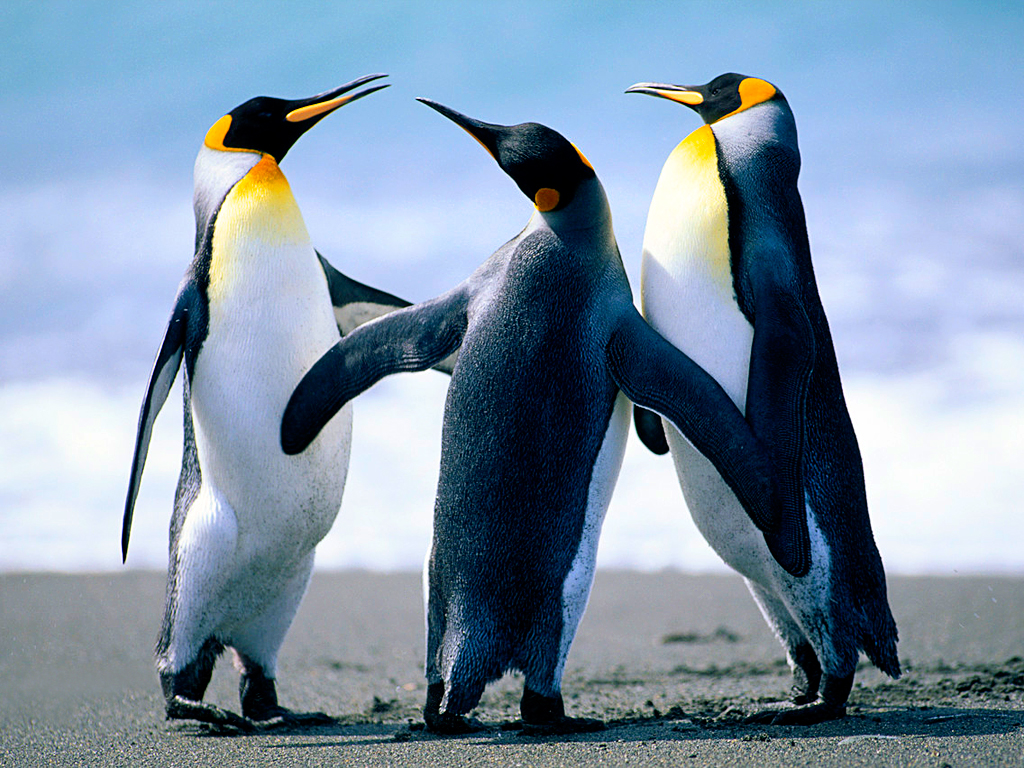
\includegraphics[scale=.50]{figures/Penguins.jpg}
\caption{TAMU figure}
\label{fig:tamu-fig6}
\end{figure}

\section{Appendix Section}


\pagebreak{}
\end{appendices}


\end{document}
